% **************************************************************************************************************
% A Classic Thesis Style
% An Homage to The Elements of Typographic Style
%
% Copyright (C) 2018 André Miede and Ivo Pletikosić
%
% If you like the style then I would appreciate a postcard. My address
% can be found in the file ClassicThesis.pdf. A collection of the
% postcards I received so far is available online at
% http://postcards.miede.de
%
% License:
% This program is free software; you can redistribute it and/or modify
% it under the terms of the GNU General Public License as published by
% the Free Software Foundation; either version 2 of the License, or
% (at your option) any later version.
%
% This program is distributed in the hope that it will be useful,
% but WITHOUT ANY WARRANTY; without even the implied warranty of
% MERCHANTABILITY or FITNESS FOR A PARTICULAR PURPOSE.  See the
% GNU General Public License for more details.
%
% You should have received a copy of the GNU General Public License
% along with this program; see the file COPYING.  If not, write to
% the Free Software Foundation, Inc., 59 Temple Place - Suite 330,
% Boston, MA 02111-1307, USA.
%
% PLEASE SEE ALSO THE AUTHORS' NOTE REGARDING THIS LICENSE
% IN THE DOCUMENTATION (ClassicThesis.pdf --> Chapter 1 / Chapter01.tex)
% **************************************************************************************************************
\RequirePackage{silence} % :-\
    \WarningFilter{scrreprt}{Usage of package `titlesec'}
    %\WarningFilter{scrreprt}{Activating an ugly workaround}
    \WarningFilter{titlesec}{Non standard sectioning command detected}
\documentclass[ twoside,openright,titlepage,numbers=noenddot,%1headlines,
                headinclude,footinclude,cleardoublepage=empty,abstract=on,
                BCOR=5mm,paper=a4,fontsize=11pt
                ]{scrreprt}

%********************************************************************
% Note: Make all your adjustments in here
%*******************************************************
% ****************************************************************************************************
% classicthesis-config.tex
% formerly known as loadpackages.sty, classicthesis-ldpkg.sty, and classicthesis-preamble.sty
% Use it at the beginning of your ClassicThesis.tex, or as a LaTeX Preamble
% in your ClassicThesis.{tex,lyx} with % ****************************************************************************************************
% classicthesis-config.tex
% formerly known as loadpackages.sty, classicthesis-ldpkg.sty, and classicthesis-preamble.sty
% Use it at the beginning of your ClassicThesis.tex, or as a LaTeX Preamble
% in your ClassicThesis.{tex,lyx} with % ****************************************************************************************************
% classicthesis-config.tex
% formerly known as loadpackages.sty, classicthesis-ldpkg.sty, and classicthesis-preamble.sty
% Use it at the beginning of your ClassicThesis.tex, or as a LaTeX Preamble
% in your ClassicThesis.{tex,lyx} with \input{classicthesis-config}
% ****************************************************************************************************
% If you like the classicthesis, then I would appreciate a postcard.
% My address can be found in the file ClassicThesis.pdf. A collection
% of the postcards I received so far is available online at
% http://postcards.miede.de
% ****************************************************************************************************


% ****************************************************************************************************
% 0. Set the encoding of your files. UTF-8 is the only sensible encoding nowadays. If you can't read
% äöüßáéçèê∂åëæƒÏ€ then change the encoding setting in your editor, not the line below. If your editor
% does not support utf8 use another editor!
% ****************************************************************************************************
\PassOptionsToPackage{utf8}{inputenc}
  \usepackage{inputenc}

\PassOptionsToPackage{T1}{fontenc} % T2A for cyrillics
  \usepackage{fontenc}


% ****************************************************************************************************
% 1. Configure classicthesis for your needs here, e.g., remove "drafting" below
% in order to deactivate the time-stamp on the pages
% (see ClassicThesis.pdf for more information):
% ****************************************************************************************************
\PassOptionsToPackage{
  drafting=false,    % print version information on the bottom of the pages
  tocaligned=false, % the left column of the toc will be aligned (no indentation)
  dottedtoc=true,  % page numbers in ToC flushed right
  eulerchapternumbers=true, % use AMS Euler for chapter font (otherwise Palatino)
  linedheaders=false,       % chaper headers will have line above and beneath
  floatperchapter=true,     % numbering per chapter for all floats (i.e., Figure 1.1)
  eulermath=false,  % use awesome Euler fonts for mathematical formulae (only with pdfLaTeX)
  beramono=true,    % toggle a nice monospaced font (w/ bold)
  palatino=true,    % deactivate standard font for loading another one, see the last section at the end of this file for suggestions
  style=classicthesis % classicthesis, arsclassica
}{classicthesis}


% ****************************************************************************************************
% 2. Personal data and user ad-hoc commands (insert your own data here)
% ****************************************************************************************************
\newcommand{\myTitle}{VAE-MAD-GAN for HIDS\xspace}
\newcommand{\mySubtitle}{ScaDS-AI \xspace}
\newcommand{\myDegree}{Bachelor Sc.\xspace}
\newcommand{\myName}{Tim Kaelble\xspace}
\newcommand{\myProf}{Prof. Rahm\xspace}
\newcommand{\myOtherProf}{ name here\xspace}
\newcommand{\mySupervisor}{Martin Grimmer\xspace}
\newcommand{\myFaculty}{Put data here\xspace}
\newcommand{\myDepartment}{Put data here\xspace}
\newcommand{\myUni}{University Leipzig\xspace}
\newcommand{\myLocation}{Leipzig\xspace}
\newcommand{\myTime}{November 2020\xspace}
%\newcommand{\myVersion}{\classicthesis}

% ********************************************************************
% Setup, finetuning, and useful commands
% ********************************************************************
\providecommand{\mLyX}{L\kern-.1667em\lower.25em\hbox{Y}\kern-.125emX\@}
\newcommand{\ie}{i.\,e.}
\newcommand{\Ie}{I.\,e.}
\newcommand{\eg}{e.\,g.}
\newcommand{\Eg}{E.\,g.}
% ****************************************************************************************************


% ****************************************************************************************************
% 3. Loading some handy packages
% ****************************************************************************************************
% ********************************************************************
% Packages with options that might require adjustments
% ********************************************************************
\PassOptionsToPackage{ngerman}{babel} % change this to your language(s), main language last
% Spanish languages need extra options in order to work with this template
%\PassOptionsToPackage{spanish,es-lcroman}{babel}
    \usepackage{babel}

\usepackage{csquotes}
\PassOptionsToPackage{%
  %backend=biber,bibencoding=utf8, %instead of bibtex
  backend=bibtex8,bibencoding=ascii,%
  language=auto,%
  style=numeric-comp,%
  %style=authoryear-comp, % Author 1999, 2010
  %bibstyle=authoryear,dashed=false, % dashed: substitute rep. author with ---
  sorting=nyt, % name, year, title
  maxbibnames=10, % default: 3, et al.
  %backref=true,%
  natbib=true % natbib compatibility mode (\citep and \citet still work)
}{biblatex}
    \usepackage{biblatex}

\PassOptionsToPackage{fleqn}{amsmath}       % math environments and more by the AMS
  \usepackage{amsmath}

% ********************************************************************
% General useful packages
% ********************************************************************
\usepackage{graphicx} %
\usepackage{scrhack} % fix warnings when using KOMA with listings package
\usepackage{xspace} % to get the spacing after macros right
\PassOptionsToPackage{printonlyused,smaller}{acronym}
  \usepackage{acronym} % nice macros for handling all acronyms in the thesis
  %\renewcommand{\bflabel}[1]{{#1}\hfill} % fix the list of acronyms --> no longer working
  %\renewcommand*{\acsfont}[1]{\textsc{#1}}
  %\renewcommand*{\aclabelfont}[1]{\acsfont{#1}}
  %\def\bflabel#1{{#1\hfill}}
  \def\bflabel#1{{\acsfont{#1}\hfill}}
  \def\aclabelfont#1{\acsfont{#1}}

% ****************************************************************************************************
% \usepackage{pgfplots} % External TikZ/PGF support (thanks to Andreas Nautsch)
% \usepackage{tikz}
%\usetikzlibrary{external}
%\tikzexternalize[mode=list and make, prefix=ext-tikz/]
% ****************************************************************************************************


% ****************************************************************************************************
% 4. Setup floats: tables, (sub)figures, and captions
% ****************************************************************************************************
\usepackage{makecell}
% \usepackage{xcolor}
% \usepackage[table]{xcolor}
\usepackage{tabularx} % better tables
  \setlength{\extrarowheight}{3pt} % increase table row height
\newcommand{\tableheadline}[1]{\multicolumn{1}{l}{\spacedlowsmallcaps{#1}}}
\newcommand{\myfloatalign}{\centering} % to be used with each float for alignment
\usepackage{subfig}
% ****************************************************************************************************


% ****************************************************************************************************
% 5. Setup code listings
% ****************************************************************************************************
\usepackage{listings}
%\lstset{emph={trueIndex,root},emphstyle=\color{BlueViolet}}%\underbar} % for special keywords
\lstset{language=[LaTeX]Tex,%C++,
  morekeywords={PassOptionsToPackage,selectlanguage},
  keywordstyle=\color{RoyalBlue},%\bfseries,
  basicstyle=\small\ttfamily,
  %identifierstyle=\color{NavyBlue},
  commentstyle=\color{Green}\ttfamily,
  stringstyle=\rmfamily,
  numbers=none,%left,%
  numberstyle=\scriptsize,%\tiny
  stepnumber=5,
  numbersep=8pt,
  showstringspaces=false,
  breaklines=true,
  %frameround=ftff,
  %frame=single,
  belowcaptionskip=.75\baselineskip
  %frame=L
}
% ****************************************************************************************************


% ****************************************************************************************************
% X. define colors
% ****************************************************************************************************


\newcolumntype{g}{>{\columncolor{Gray!16}}l}

% ****************************************************************************************************
% 6. Last calls before the bar closes
% ****************************************************************************************************
% ********************************************************************
% Her Majesty herself
% ********************************************************************
\usepackage{classicthesis}
\setcounter{secnumdepth}{3}

% ********************************************************************
% Fine-tune hyperreferences (hyperref should be called last)
% ********************************************************************
\hypersetup{%
  %draft, % hyperref's draft mode, for printing see below
  colorlinks=true, linktocpage=true, pdfstartpage=3, pdfstartview=FitV,%
  % uncomment the following line if you want to have black links (e.g., for printing)
  %colorlinks=false, linktocpage=false, pdfstartpage=3, pdfstartview=FitV, pdfborder={0 0 0},%
  breaklinks=true, pageanchor=true,%
  pdfpagemode=UseNone, %
  % pdfpagemode=UseOutlines,%
  plainpages=false, bookmarksnumbered, bookmarksopen=true, bookmarksopenlevel=1,%
  hypertexnames=true, pdfhighlight=/O,%nesting=true,%frenchlinks,%
  urlcolor=CTurl, linkcolor=CTlink, citecolor=CTcitation, %pagecolor=RoyalBlue,%
  %urlcolor=Black, linkcolor=Black, citecolor=Black, %pagecolor=Black,%
  pdftitle={\myTitle},%
  pdfauthor={\textcopyright\ \myName, \myUni, \myFaculty},%
  pdfsubject={},%
  pdfkeywords={},%
  pdfcreator={pdfLaTeX},%
  pdfproducer={LaTeX with hyperref and classicthesis}%
}


% ********************************************************************
% Setup autoreferences (hyperref and babel)
% ********************************************************************
% There are some issues regarding autorefnames
% http://www.tex.ac.uk/cgi-bin/texfaq2html?label=latexwords
% you have to redefine the macros for the
% language you use, e.g., american, ngerman
% (as chosen when loading babel/AtBeginDocument)
% ********************************************************************
\makeatletter
\@ifpackageloaded{babel}%
  {%
    \addto\extrasamerican{%
      %\renewcommand*{\figureautorefname}{Figure}%
      %\renewcommand*{\tableautorefname}{Table}%
      %\renewcommand*{\partautorefname}{Part}%
      %\renewcommand*{\chapterautorefname}{Chapter}%
      %\renewcommand*{\sectionautorefname}{Section}%
      %\renewcommand*{\subsectionautorefname}{Section}%
      %\renewcommand*{\subsubsectionautorefname}{Section}%
      \renewcommand*{\subsubsectionautorefname}{Abschnitt}%
      \renewcommand*{\subsectionautorefname}{Abschnitt}%
      \renewcommand*{\sectionautorefname}{Abschnitt}%
      \renewcommand*{\chapterautorefname}{Kapitel}%
      \renewcommand*{\figureautorefname}{Abbildung}%
      \renewcommand*{\tableautorefname}{Tabelle}%
      \renewcommand*{\paragraphautorefname}{Absatz}%
      \renewcommand*{\subparagraphautorefname}{Unterabsatz}%
      \renewcommand*{\footnoteautorefname}{Fußnote}%
      \renewcommand*{\FancyVerbLineautorefname}{Zeile}%
      \renewcommand*{\theoremautorefname}{Theorem}%
      \renewcommand*{\appendixautorefname}{Anhang}%
      \renewcommand*{\equationautorefname}{Gleichung}%
      \renewcommand*{\itemautorefname}{Punkt}%
    }%
    \addto\extrasngerman{%
      \renewcommand*{\paragraphautorefname}{Absatz}%
      \renewcommand*{\subparagraphautorefname}{Unterabsatz}%
      \renewcommand*{\footnoteautorefname}{Fu\"snote}%
      \renewcommand*{\FancyVerbLineautorefname}{Zeile}%
      \renewcommand*{\theoremautorefname}{Theorem}%
      \renewcommand*{\appendixautorefname}{Anhang}%
      \renewcommand*{\equationautorefname}{Gleichung}%
      \renewcommand*{\itemautorefname}{Punkt}%
    }%
      % Fix to getting autorefs for subfigures right (thanks to Belinda Vogt for changing the definition)
      \providecommand{\subfigureautorefname}{\figureautorefname}%
    }{\relax}
\makeatother


% ********************************************************************
% Development Stuff
% ********************************************************************
\listfiles
%\PassOptionsToPackage{l2tabu,orthodox,abort}{nag}
%  \usepackage{nag}
%\PassOptionsToPackage{warning, all}{onlyamsmath}
%  \usepackage{onlyamsmath}
\renewcommand{\arraystretch}{1}

% ****************************************************************************************************
% 7. Further adjustments (experimental)
% ****************************************************************************************************
% ********************************************************************
% Changing the text area
% ********************************************************************
%\areaset[current]{312pt}{761pt} % 686 (factor 2.2) + 33 head + 42 head \the\footskip
%\setlength{\marginparwidth}{7em}%
%\setlength{\marginparsep}{2em}%

% ********************************************************************
% Using different fonts
% ********************************************************************
%\usepackage[oldstylenums]{kpfonts} % oldstyle notextcomp
% \usepackage[osf]{libertine}
%\usepackage[light,condensed,math]{iwona}
%\renewcommand{\sfdefault}{iwona}
%\usepackage{lmodern} % <-- no osf support :-(
%\usepackage{cfr-lm} %
%\usepackage[urw-garamond]{mathdesign} <-- no osf support :-(
%\usepackage[default,osfigures]{opensans} % scale=0.95
%\usepackage[sfdefault]{FiraSans}
% \usepackage[opticals,mathlf]{MinionPro} % onlytext
% ********************************************************************
%\usepackage[largesc,osf]{newpxtext}
%\linespread{1.05} % a bit more for Palatino
% Used to fix these:
% https://bitbucket.org/amiede/classicthesis/issues/139/italics-in-pallatino-capitals-chapter
% https://bitbucket.org/amiede/classicthesis/issues/45/problema-testatine-su-classicthesis-style
% ********************************************************************
% ****************************************************************************************************

% ****************************************************************************************************
% If you like the classicthesis, then I would appreciate a postcard.
% My address can be found in the file ClassicThesis.pdf. A collection
% of the postcards I received so far is available online at
% http://postcards.miede.de
% ****************************************************************************************************


% ****************************************************************************************************
% 0. Set the encoding of your files. UTF-8 is the only sensible encoding nowadays. If you can't read
% äöüßáéçèê∂åëæƒÏ€ then change the encoding setting in your editor, not the line below. If your editor
% does not support utf8 use another editor!
% ****************************************************************************************************
\PassOptionsToPackage{utf8}{inputenc}
  \usepackage{inputenc}

\PassOptionsToPackage{T1}{fontenc} % T2A for cyrillics
  \usepackage{fontenc}


% ****************************************************************************************************
% 1. Configure classicthesis for your needs here, e.g., remove "drafting" below
% in order to deactivate the time-stamp on the pages
% (see ClassicThesis.pdf for more information):
% ****************************************************************************************************
\PassOptionsToPackage{
  drafting=false,    % print version information on the bottom of the pages
  tocaligned=false, % the left column of the toc will be aligned (no indentation)
  dottedtoc=true,  % page numbers in ToC flushed right
  eulerchapternumbers=true, % use AMS Euler for chapter font (otherwise Palatino)
  linedheaders=false,       % chaper headers will have line above and beneath
  floatperchapter=true,     % numbering per chapter for all floats (i.e., Figure 1.1)
  eulermath=false,  % use awesome Euler fonts for mathematical formulae (only with pdfLaTeX)
  beramono=true,    % toggle a nice monospaced font (w/ bold)
  palatino=true,    % deactivate standard font for loading another one, see the last section at the end of this file for suggestions
  style=classicthesis % classicthesis, arsclassica
}{classicthesis}


% ****************************************************************************************************
% 2. Personal data and user ad-hoc commands (insert your own data here)
% ****************************************************************************************************
\newcommand{\myTitle}{VAE-MAD-GAN for HIDS\xspace}
\newcommand{\mySubtitle}{ScaDS-AI \xspace}
\newcommand{\myDegree}{Bachelor Sc.\xspace}
\newcommand{\myName}{Tim Kaelble\xspace}
\newcommand{\myProf}{Prof. Rahm\xspace}
\newcommand{\myOtherProf}{ name here\xspace}
\newcommand{\mySupervisor}{Martin Grimmer\xspace}
\newcommand{\myFaculty}{Put data here\xspace}
\newcommand{\myDepartment}{Put data here\xspace}
\newcommand{\myUni}{University Leipzig\xspace}
\newcommand{\myLocation}{Leipzig\xspace}
\newcommand{\myTime}{November 2020\xspace}
%\newcommand{\myVersion}{\classicthesis}

% ********************************************************************
% Setup, finetuning, and useful commands
% ********************************************************************
\providecommand{\mLyX}{L\kern-.1667em\lower.25em\hbox{Y}\kern-.125emX\@}
\newcommand{\ie}{i.\,e.}
\newcommand{\Ie}{I.\,e.}
\newcommand{\eg}{e.\,g.}
\newcommand{\Eg}{E.\,g.}
% ****************************************************************************************************


% ****************************************************************************************************
% 3. Loading some handy packages
% ****************************************************************************************************
% ********************************************************************
% Packages with options that might require adjustments
% ********************************************************************
\PassOptionsToPackage{ngerman}{babel} % change this to your language(s), main language last
% Spanish languages need extra options in order to work with this template
%\PassOptionsToPackage{spanish,es-lcroman}{babel}
    \usepackage{babel}

\usepackage{csquotes}
\PassOptionsToPackage{%
  %backend=biber,bibencoding=utf8, %instead of bibtex
  backend=bibtex8,bibencoding=ascii,%
  language=auto,%
  style=numeric-comp,%
  %style=authoryear-comp, % Author 1999, 2010
  %bibstyle=authoryear,dashed=false, % dashed: substitute rep. author with ---
  sorting=nyt, % name, year, title
  maxbibnames=10, % default: 3, et al.
  %backref=true,%
  natbib=true % natbib compatibility mode (\citep and \citet still work)
}{biblatex}
    \usepackage{biblatex}

\PassOptionsToPackage{fleqn}{amsmath}       % math environments and more by the AMS
  \usepackage{amsmath}

% ********************************************************************
% General useful packages
% ********************************************************************
\usepackage{graphicx} %
\usepackage{scrhack} % fix warnings when using KOMA with listings package
\usepackage{xspace} % to get the spacing after macros right
\PassOptionsToPackage{printonlyused,smaller}{acronym}
  \usepackage{acronym} % nice macros for handling all acronyms in the thesis
  %\renewcommand{\bflabel}[1]{{#1}\hfill} % fix the list of acronyms --> no longer working
  %\renewcommand*{\acsfont}[1]{\textsc{#1}}
  %\renewcommand*{\aclabelfont}[1]{\acsfont{#1}}
  %\def\bflabel#1{{#1\hfill}}
  \def\bflabel#1{{\acsfont{#1}\hfill}}
  \def\aclabelfont#1{\acsfont{#1}}

% ****************************************************************************************************
% \usepackage{pgfplots} % External TikZ/PGF support (thanks to Andreas Nautsch)
% \usepackage{tikz}
%\usetikzlibrary{external}
%\tikzexternalize[mode=list and make, prefix=ext-tikz/]
% ****************************************************************************************************


% ****************************************************************************************************
% 4. Setup floats: tables, (sub)figures, and captions
% ****************************************************************************************************
\usepackage{makecell}
% \usepackage{xcolor}
% \usepackage[table]{xcolor}
\usepackage{tabularx} % better tables
  \setlength{\extrarowheight}{3pt} % increase table row height
\newcommand{\tableheadline}[1]{\multicolumn{1}{l}{\spacedlowsmallcaps{#1}}}
\newcommand{\myfloatalign}{\centering} % to be used with each float for alignment
\usepackage{subfig}
% ****************************************************************************************************


% ****************************************************************************************************
% 5. Setup code listings
% ****************************************************************************************************
\usepackage{listings}
%\lstset{emph={trueIndex,root},emphstyle=\color{BlueViolet}}%\underbar} % for special keywords
\lstset{language=[LaTeX]Tex,%C++,
  morekeywords={PassOptionsToPackage,selectlanguage},
  keywordstyle=\color{RoyalBlue},%\bfseries,
  basicstyle=\small\ttfamily,
  %identifierstyle=\color{NavyBlue},
  commentstyle=\color{Green}\ttfamily,
  stringstyle=\rmfamily,
  numbers=none,%left,%
  numberstyle=\scriptsize,%\tiny
  stepnumber=5,
  numbersep=8pt,
  showstringspaces=false,
  breaklines=true,
  %frameround=ftff,
  %frame=single,
  belowcaptionskip=.75\baselineskip
  %frame=L
}
% ****************************************************************************************************


% ****************************************************************************************************
% X. define colors
% ****************************************************************************************************


\newcolumntype{g}{>{\columncolor{Gray!16}}l}

% ****************************************************************************************************
% 6. Last calls before the bar closes
% ****************************************************************************************************
% ********************************************************************
% Her Majesty herself
% ********************************************************************
\usepackage{classicthesis}
\setcounter{secnumdepth}{3}

% ********************************************************************
% Fine-tune hyperreferences (hyperref should be called last)
% ********************************************************************
\hypersetup{%
  %draft, % hyperref's draft mode, for printing see below
  colorlinks=true, linktocpage=true, pdfstartpage=3, pdfstartview=FitV,%
  % uncomment the following line if you want to have black links (e.g., for printing)
  %colorlinks=false, linktocpage=false, pdfstartpage=3, pdfstartview=FitV, pdfborder={0 0 0},%
  breaklinks=true, pageanchor=true,%
  pdfpagemode=UseNone, %
  % pdfpagemode=UseOutlines,%
  plainpages=false, bookmarksnumbered, bookmarksopen=true, bookmarksopenlevel=1,%
  hypertexnames=true, pdfhighlight=/O,%nesting=true,%frenchlinks,%
  urlcolor=CTurl, linkcolor=CTlink, citecolor=CTcitation, %pagecolor=RoyalBlue,%
  %urlcolor=Black, linkcolor=Black, citecolor=Black, %pagecolor=Black,%
  pdftitle={\myTitle},%
  pdfauthor={\textcopyright\ \myName, \myUni, \myFaculty},%
  pdfsubject={},%
  pdfkeywords={},%
  pdfcreator={pdfLaTeX},%
  pdfproducer={LaTeX with hyperref and classicthesis}%
}


% ********************************************************************
% Setup autoreferences (hyperref and babel)
% ********************************************************************
% There are some issues regarding autorefnames
% http://www.tex.ac.uk/cgi-bin/texfaq2html?label=latexwords
% you have to redefine the macros for the
% language you use, e.g., american, ngerman
% (as chosen when loading babel/AtBeginDocument)
% ********************************************************************
\makeatletter
\@ifpackageloaded{babel}%
  {%
    \addto\extrasamerican{%
      %\renewcommand*{\figureautorefname}{Figure}%
      %\renewcommand*{\tableautorefname}{Table}%
      %\renewcommand*{\partautorefname}{Part}%
      %\renewcommand*{\chapterautorefname}{Chapter}%
      %\renewcommand*{\sectionautorefname}{Section}%
      %\renewcommand*{\subsectionautorefname}{Section}%
      %\renewcommand*{\subsubsectionautorefname}{Section}%
      \renewcommand*{\subsubsectionautorefname}{Abschnitt}%
      \renewcommand*{\subsectionautorefname}{Abschnitt}%
      \renewcommand*{\sectionautorefname}{Abschnitt}%
      \renewcommand*{\chapterautorefname}{Kapitel}%
      \renewcommand*{\figureautorefname}{Abbildung}%
      \renewcommand*{\tableautorefname}{Tabelle}%
      \renewcommand*{\paragraphautorefname}{Absatz}%
      \renewcommand*{\subparagraphautorefname}{Unterabsatz}%
      \renewcommand*{\footnoteautorefname}{Fußnote}%
      \renewcommand*{\FancyVerbLineautorefname}{Zeile}%
      \renewcommand*{\theoremautorefname}{Theorem}%
      \renewcommand*{\appendixautorefname}{Anhang}%
      \renewcommand*{\equationautorefname}{Gleichung}%
      \renewcommand*{\itemautorefname}{Punkt}%
    }%
    \addto\extrasngerman{%
      \renewcommand*{\paragraphautorefname}{Absatz}%
      \renewcommand*{\subparagraphautorefname}{Unterabsatz}%
      \renewcommand*{\footnoteautorefname}{Fu\"snote}%
      \renewcommand*{\FancyVerbLineautorefname}{Zeile}%
      \renewcommand*{\theoremautorefname}{Theorem}%
      \renewcommand*{\appendixautorefname}{Anhang}%
      \renewcommand*{\equationautorefname}{Gleichung}%
      \renewcommand*{\itemautorefname}{Punkt}%
    }%
      % Fix to getting autorefs for subfigures right (thanks to Belinda Vogt for changing the definition)
      \providecommand{\subfigureautorefname}{\figureautorefname}%
    }{\relax}
\makeatother


% ********************************************************************
% Development Stuff
% ********************************************************************
\listfiles
%\PassOptionsToPackage{l2tabu,orthodox,abort}{nag}
%  \usepackage{nag}
%\PassOptionsToPackage{warning, all}{onlyamsmath}
%  \usepackage{onlyamsmath}
\renewcommand{\arraystretch}{1}

% ****************************************************************************************************
% 7. Further adjustments (experimental)
% ****************************************************************************************************
% ********************************************************************
% Changing the text area
% ********************************************************************
%\areaset[current]{312pt}{761pt} % 686 (factor 2.2) + 33 head + 42 head \the\footskip
%\setlength{\marginparwidth}{7em}%
%\setlength{\marginparsep}{2em}%

% ********************************************************************
% Using different fonts
% ********************************************************************
%\usepackage[oldstylenums]{kpfonts} % oldstyle notextcomp
% \usepackage[osf]{libertine}
%\usepackage[light,condensed,math]{iwona}
%\renewcommand{\sfdefault}{iwona}
%\usepackage{lmodern} % <-- no osf support :-(
%\usepackage{cfr-lm} %
%\usepackage[urw-garamond]{mathdesign} <-- no osf support :-(
%\usepackage[default,osfigures]{opensans} % scale=0.95
%\usepackage[sfdefault]{FiraSans}
% \usepackage[opticals,mathlf]{MinionPro} % onlytext
% ********************************************************************
%\usepackage[largesc,osf]{newpxtext}
%\linespread{1.05} % a bit more for Palatino
% Used to fix these:
% https://bitbucket.org/amiede/classicthesis/issues/139/italics-in-pallatino-capitals-chapter
% https://bitbucket.org/amiede/classicthesis/issues/45/problema-testatine-su-classicthesis-style
% ********************************************************************
% ****************************************************************************************************

% ****************************************************************************************************
% If you like the classicthesis, then I would appreciate a postcard.
% My address can be found in the file ClassicThesis.pdf. A collection
% of the postcards I received so far is available online at
% http://postcards.miede.de
% ****************************************************************************************************


% ****************************************************************************************************
% 0. Set the encoding of your files. UTF-8 is the only sensible encoding nowadays. If you can't read
% äöüßáéçèê∂åëæƒÏ€ then change the encoding setting in your editor, not the line below. If your editor
% does not support utf8 use another editor!
% ****************************************************************************************************
\PassOptionsToPackage{utf8}{inputenc}
  \usepackage{inputenc}

\PassOptionsToPackage{T1}{fontenc} % T2A for cyrillics
  \usepackage{fontenc}


% ****************************************************************************************************
% 1. Configure classicthesis for your needs here, e.g., remove "drafting" below
% in order to deactivate the time-stamp on the pages
% (see ClassicThesis.pdf for more information):
% ****************************************************************************************************
\PassOptionsToPackage{
  drafting=false,    % print version information on the bottom of the pages
  tocaligned=false, % the left column of the toc will be aligned (no indentation)
  dottedtoc=true,  % page numbers in ToC flushed right
  eulerchapternumbers=true, % use AMS Euler for chapter font (otherwise Palatino)
  linedheaders=false,       % chaper headers will have line above and beneath
  floatperchapter=true,     % numbering per chapter for all floats (i.e., Figure 1.1)
  eulermath=false,  % use awesome Euler fonts for mathematical formulae (only with pdfLaTeX)
  beramono=true,    % toggle a nice monospaced font (w/ bold)
  palatino=true,    % deactivate standard font for loading another one, see the last section at the end of this file for suggestions
  style=classicthesis % classicthesis, arsclassica
}{classicthesis}


% ****************************************************************************************************
% 2. Personal data and user ad-hoc commands (insert your own data here)
% ****************************************************************************************************
\newcommand{\myTitle}{VAE-MAD-GAN for HIDS\xspace}
\newcommand{\mySubtitle}{ScaDS-AI \xspace}
\newcommand{\myDegree}{Bachelor Sc.\xspace}
\newcommand{\myName}{Tim Kaelble\xspace}
\newcommand{\myProf}{Prof. Rahm\xspace}
\newcommand{\myOtherProf}{ name here\xspace}
\newcommand{\mySupervisor}{Martin Grimmer\xspace}
\newcommand{\myFaculty}{Put data here\xspace}
\newcommand{\myDepartment}{Put data here\xspace}
\newcommand{\myUni}{University Leipzig\xspace}
\newcommand{\myLocation}{Leipzig\xspace}
\newcommand{\myTime}{November 2020\xspace}
%\newcommand{\myVersion}{\classicthesis}

% ********************************************************************
% Setup, finetuning, and useful commands
% ********************************************************************
\providecommand{\mLyX}{L\kern-.1667em\lower.25em\hbox{Y}\kern-.125emX\@}
\newcommand{\ie}{i.\,e.}
\newcommand{\Ie}{I.\,e.}
\newcommand{\eg}{e.\,g.}
\newcommand{\Eg}{E.\,g.}
% ****************************************************************************************************


% ****************************************************************************************************
% 3. Loading some handy packages
% ****************************************************************************************************
% ********************************************************************
% Packages with options that might require adjustments
% ********************************************************************
\PassOptionsToPackage{ngerman}{babel} % change this to your language(s), main language last
% Spanish languages need extra options in order to work with this template
%\PassOptionsToPackage{spanish,es-lcroman}{babel}
    \usepackage{babel}

\usepackage{csquotes}
\PassOptionsToPackage{%
  %backend=biber,bibencoding=utf8, %instead of bibtex
  backend=bibtex8,bibencoding=ascii,%
  language=auto,%
  style=numeric-comp,%
  %style=authoryear-comp, % Author 1999, 2010
  %bibstyle=authoryear,dashed=false, % dashed: substitute rep. author with ---
  sorting=nyt, % name, year, title
  maxbibnames=10, % default: 3, et al.
  %backref=true,%
  natbib=true % natbib compatibility mode (\citep and \citet still work)
}{biblatex}
    \usepackage{biblatex}

\PassOptionsToPackage{fleqn}{amsmath}       % math environments and more by the AMS
  \usepackage{amsmath}

% ********************************************************************
% General useful packages
% ********************************************************************
\usepackage{graphicx} %
\usepackage{scrhack} % fix warnings when using KOMA with listings package
\usepackage{xspace} % to get the spacing after macros right
\PassOptionsToPackage{printonlyused,smaller}{acronym}
  \usepackage{acronym} % nice macros for handling all acronyms in the thesis
  %\renewcommand{\bflabel}[1]{{#1}\hfill} % fix the list of acronyms --> no longer working
  %\renewcommand*{\acsfont}[1]{\textsc{#1}}
  %\renewcommand*{\aclabelfont}[1]{\acsfont{#1}}
  %\def\bflabel#1{{#1\hfill}}
  \def\bflabel#1{{\acsfont{#1}\hfill}}
  \def\aclabelfont#1{\acsfont{#1}}

% ****************************************************************************************************
% \usepackage{pgfplots} % External TikZ/PGF support (thanks to Andreas Nautsch)
% \usepackage{tikz}
%\usetikzlibrary{external}
%\tikzexternalize[mode=list and make, prefix=ext-tikz/]
% ****************************************************************************************************


% ****************************************************************************************************
% 4. Setup floats: tables, (sub)figures, and captions
% ****************************************************************************************************
\usepackage{makecell}
% \usepackage{xcolor}
% \usepackage[table]{xcolor}
\usepackage{tabularx} % better tables
  \setlength{\extrarowheight}{3pt} % increase table row height
\newcommand{\tableheadline}[1]{\multicolumn{1}{l}{\spacedlowsmallcaps{#1}}}
\newcommand{\myfloatalign}{\centering} % to be used with each float for alignment
\usepackage{subfig}
% ****************************************************************************************************


% ****************************************************************************************************
% 5. Setup code listings
% ****************************************************************************************************
\usepackage{listings}
%\lstset{emph={trueIndex,root},emphstyle=\color{BlueViolet}}%\underbar} % for special keywords
\lstset{language=[LaTeX]Tex,%C++,
  morekeywords={PassOptionsToPackage,selectlanguage},
  keywordstyle=\color{RoyalBlue},%\bfseries,
  basicstyle=\small\ttfamily,
  %identifierstyle=\color{NavyBlue},
  commentstyle=\color{Green}\ttfamily,
  stringstyle=\rmfamily,
  numbers=none,%left,%
  numberstyle=\scriptsize,%\tiny
  stepnumber=5,
  numbersep=8pt,
  showstringspaces=false,
  breaklines=true,
  %frameround=ftff,
  %frame=single,
  belowcaptionskip=.75\baselineskip
  %frame=L
}
% ****************************************************************************************************


% ****************************************************************************************************
% X. define colors
% ****************************************************************************************************


\newcolumntype{g}{>{\columncolor{Gray!16}}l}

% ****************************************************************************************************
% 6. Last calls before the bar closes
% ****************************************************************************************************
% ********************************************************************
% Her Majesty herself
% ********************************************************************
\usepackage{classicthesis}
\setcounter{secnumdepth}{3}

% ********************************************************************
% Fine-tune hyperreferences (hyperref should be called last)
% ********************************************************************
\hypersetup{%
  %draft, % hyperref's draft mode, for printing see below
  colorlinks=true, linktocpage=true, pdfstartpage=3, pdfstartview=FitV,%
  % uncomment the following line if you want to have black links (e.g., for printing)
  %colorlinks=false, linktocpage=false, pdfstartpage=3, pdfstartview=FitV, pdfborder={0 0 0},%
  breaklinks=true, pageanchor=true,%
  pdfpagemode=UseNone, %
  % pdfpagemode=UseOutlines,%
  plainpages=false, bookmarksnumbered, bookmarksopen=true, bookmarksopenlevel=1,%
  hypertexnames=true, pdfhighlight=/O,%nesting=true,%frenchlinks,%
  urlcolor=CTurl, linkcolor=CTlink, citecolor=CTcitation, %pagecolor=RoyalBlue,%
  %urlcolor=Black, linkcolor=Black, citecolor=Black, %pagecolor=Black,%
  pdftitle={\myTitle},%
  pdfauthor={\textcopyright\ \myName, \myUni, \myFaculty},%
  pdfsubject={},%
  pdfkeywords={},%
  pdfcreator={pdfLaTeX},%
  pdfproducer={LaTeX with hyperref and classicthesis}%
}


% ********************************************************************
% Setup autoreferences (hyperref and babel)
% ********************************************************************
% There are some issues regarding autorefnames
% http://www.tex.ac.uk/cgi-bin/texfaq2html?label=latexwords
% you have to redefine the macros for the
% language you use, e.g., american, ngerman
% (as chosen when loading babel/AtBeginDocument)
% ********************************************************************
\makeatletter
\@ifpackageloaded{babel}%
  {%
    \addto\extrasamerican{%
      %\renewcommand*{\figureautorefname}{Figure}%
      %\renewcommand*{\tableautorefname}{Table}%
      %\renewcommand*{\partautorefname}{Part}%
      %\renewcommand*{\chapterautorefname}{Chapter}%
      %\renewcommand*{\sectionautorefname}{Section}%
      %\renewcommand*{\subsectionautorefname}{Section}%
      %\renewcommand*{\subsubsectionautorefname}{Section}%
      \renewcommand*{\subsubsectionautorefname}{Abschnitt}%
      \renewcommand*{\subsectionautorefname}{Abschnitt}%
      \renewcommand*{\sectionautorefname}{Abschnitt}%
      \renewcommand*{\chapterautorefname}{Kapitel}%
      \renewcommand*{\figureautorefname}{Abbildung}%
      \renewcommand*{\tableautorefname}{Tabelle}%
      \renewcommand*{\paragraphautorefname}{Absatz}%
      \renewcommand*{\subparagraphautorefname}{Unterabsatz}%
      \renewcommand*{\footnoteautorefname}{Fußnote}%
      \renewcommand*{\FancyVerbLineautorefname}{Zeile}%
      \renewcommand*{\theoremautorefname}{Theorem}%
      \renewcommand*{\appendixautorefname}{Anhang}%
      \renewcommand*{\equationautorefname}{Gleichung}%
      \renewcommand*{\itemautorefname}{Punkt}%
    }%
    \addto\extrasngerman{%
      \renewcommand*{\paragraphautorefname}{Absatz}%
      \renewcommand*{\subparagraphautorefname}{Unterabsatz}%
      \renewcommand*{\footnoteautorefname}{Fu\"snote}%
      \renewcommand*{\FancyVerbLineautorefname}{Zeile}%
      \renewcommand*{\theoremautorefname}{Theorem}%
      \renewcommand*{\appendixautorefname}{Anhang}%
      \renewcommand*{\equationautorefname}{Gleichung}%
      \renewcommand*{\itemautorefname}{Punkt}%
    }%
      % Fix to getting autorefs for subfigures right (thanks to Belinda Vogt for changing the definition)
      \providecommand{\subfigureautorefname}{\figureautorefname}%
    }{\relax}
\makeatother


% ********************************************************************
% Development Stuff
% ********************************************************************
\listfiles
%\PassOptionsToPackage{l2tabu,orthodox,abort}{nag}
%  \usepackage{nag}
%\PassOptionsToPackage{warning, all}{onlyamsmath}
%  \usepackage{onlyamsmath}
\renewcommand{\arraystretch}{1}

% ****************************************************************************************************
% 7. Further adjustments (experimental)
% ****************************************************************************************************
% ********************************************************************
% Changing the text area
% ********************************************************************
%\areaset[current]{312pt}{761pt} % 686 (factor 2.2) + 33 head + 42 head \the\footskip
%\setlength{\marginparwidth}{7em}%
%\setlength{\marginparsep}{2em}%

% ********************************************************************
% Using different fonts
% ********************************************************************
%\usepackage[oldstylenums]{kpfonts} % oldstyle notextcomp
% \usepackage[osf]{libertine}
%\usepackage[light,condensed,math]{iwona}
%\renewcommand{\sfdefault}{iwona}
%\usepackage{lmodern} % <-- no osf support :-(
%\usepackage{cfr-lm} %
%\usepackage[urw-garamond]{mathdesign} <-- no osf support :-(
%\usepackage[default,osfigures]{opensans} % scale=0.95
%\usepackage[sfdefault]{FiraSans}
% \usepackage[opticals,mathlf]{MinionPro} % onlytext
% ********************************************************************
%\usepackage[largesc,osf]{newpxtext}
%\linespread{1.05} % a bit more for Palatino
% Used to fix these:
% https://bitbucket.org/amiede/classicthesis/issues/139/italics-in-pallatino-capitals-chapter
% https://bitbucket.org/amiede/classicthesis/issues/45/problema-testatine-su-classicthesis-style
% ********************************************************************
% ****************************************************************************************************


%********************************************************************
% Bibliographies
%*******************************************************
\addbibresource{Bibliography.bib}
%\addbibresource[label=ownpubs]{AMiede_Publications.bib}

%********************************************************************
% Hyphenation
%*******************************************************
%\hyphenation{put special hyphenation here}

% ********************************************************************
% GO!GO!GO! MOVE IT!
%*******************************************************
%\usepackage[ngerman]{babel}
%\addto{\captionsngerman}{%
  %\renewcommand*{\contentsname}{Inhalt}
  %\renewcommand*{\listfigurename}{Abbildungen}
  %\renewcommand*{\listtablename}{Tabellen}
  %\renewcommand*{\figurename}{Abbildung}
  %\renewcommand*{\tablename}{Tabelle}
%}
%\renewcommand{\listfigurename}{Abbildungsverzeichnis}
%\renewcommand{\listtablename}{Tabellenverzeichnis}
%\renewcommand{\contentsname}{Inhaltsverzeichnis}
\begin{document}
\frenchspacing
\raggedbottom
%\selectlanguage{ngerman, american} % american ngerman
%\renewcommand*{\bibname}{new name}
%\setbibpreamble{}
\pagenumbering{roman}
\pagestyle{plain}
%********************************************************************
% Frontmatter
%*******************************************************
%%*******************************************************
% Little Dirty Titlepage
%*******************************************************
\thispagestyle{empty}
%\pdfbookmark[1]{Titel}{title}
%*******************************************************
\begin{center}
    \spacedlowsmallcaps{\myName} \\ \medskip

    \begingroup
        \color{CTtitle}\spacedallcaps{\myTitle}
    \endgroup
\end{center}

%*******************************************************
% Titlepage
%*******************************************************
\begin{titlepage}
    %\pdfbookmark[1]{\myTitle}{titlepage}
    % if you want the titlepage to be centered, uncomment and fine-tune the line below (KOMA classes environment)
    \begin{addmargin}[-1cm]{-3cm}
    \begin{center}
        \large

        \hfill

        \vfill

        \begingroup
            \color{CTtitle}\spacedallcaps{\myTitle} \\ \bigskip
        \endgroup

        \spacedlowsmallcaps{\myName}

        \vfill

        %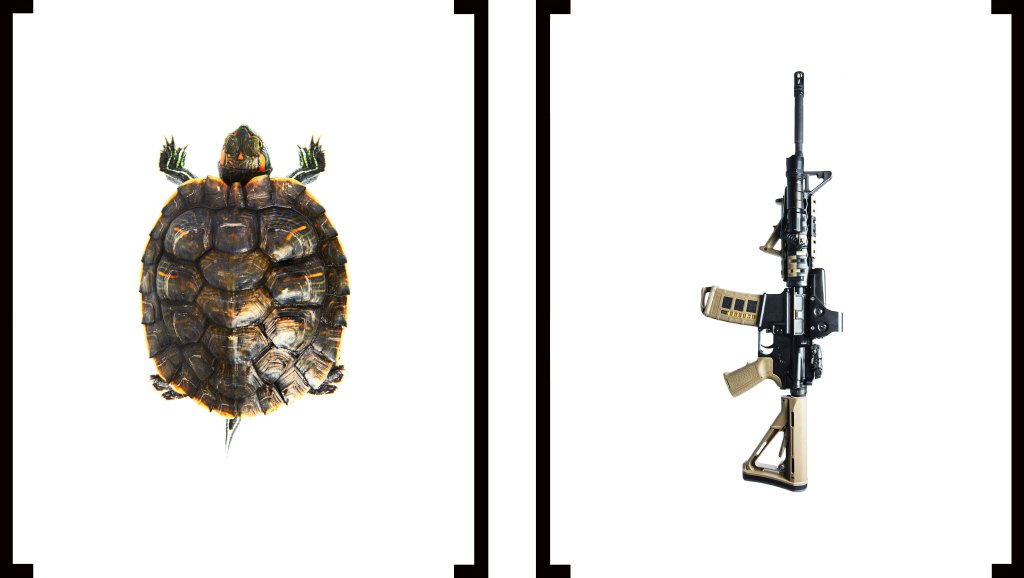
\includegraphics[width=6cm]{gfx/turtle_rifle.jpg} \\ \medskip

        \mySubtitle \\ \medskip
        %\myDegree \\
        %\myDepartment \\
        %\myFaculty \\
        %\myUni \\ \bigskip

        \myTime\ -- \myVersion

        \vfill

    \end{center}
  \end{addmargin}
\end{titlepage}

\thispagestyle{empty}

\hfill

\vfill

\noindent\myName: \textit{\myTitle,} \mySubtitle, %\myDegree,
\textcopyright\ \myTime

%\bigskip
%
%\noindent\spacedlowsmallcaps{Supervisors}: \\
%\myProf \\
%\myOtherProf \\
%\mySupervisor
%
%\medskip
%
%\noindent\spacedlowsmallcaps{Location}: \\
%\myLocation
%
%\medskip
%
%\noindent\spacedlowsmallcaps{Time Frame}: \\
%\myTime

%\cleardoublepage%*******************************************************
% Dedication
%*******************************************************
\thispagestyle{empty}
\phantomsection
\pdfbookmark[1]{Dedication}{Dedication}

\vspace*{3cm}

\begin{center}
    \emph{Ohana} means family. \\
    Family means nobody gets left behind, or forgotten. \\ \medskip
    --- Lilo \& Stitch
\end{center}

\medskip

\begin{center}
    Dedicated to the loving memory of Rudolf Miede. \\ \smallskip
    1939\,--\,2005
\end{center}

%\cleardoublepage\include{FrontBackmatter/Foreword}
%*******************************************************
% Abstract
%*******************************************************
%\renewcommand{\abstractname}{Abstract}
\pdfbookmark[1]{Abstract}{Abstract}
% \addcontentsline{toc}{chapter}{\tocEntry{Abstract}}
\begingroup
\let\clearpage\relax
\let\cleardoublepage\relax
\let\cleardoublepage\relax

\chapter*{Abstract}
 The increase in zero-day attacks on computer systems poses new challenges for IT security research.
 Intrusion detection systems (IDSs) are designed to alert operators to any attacks in real time.
 Anomaly-based IDS is specifically targeted to detect zero-day attacks as well.
 In this thesis, an anomaly-based Host-based Intrusion Detection System (HIDS) based on Long-Short-Term-Memory neural networks (LSTMs) is developed.
 For this purpose, the sequence of system call data is investigated.
 In a further iteration, novel methods are presented with which the sequences are extended by additional system call parameters.
 This work investigates whether the LSTMs are successful in anomaly-based HIDS.\@
 Additionally, it will be investigated which extra parameters can be used to improve the results of the developed algorithm.
 It was shown in this work that the LSTM approach provides competitive results, but does so at a significant computational cost.
 The developed additional parameters could achieve a significant improvement of the results and could also find their use in connection with other algorithms.

\vfill

\begin{otherlanguage}{ngerman}
\pdfbookmark[1]{Zusammenfassung}{Zusammenfassung}
\chapter*{Zusammenfassung}
Die Zunahme von Zero-Day Angriffen auf Computer Systeme stellt die IT-Sicherheitsforschung vor neue Herausforderungen.
Intrusion Detection Systems (IDSs) sollen die Betreibenden möglichst in Echtzeit auf jegliche Angriffe hinweisen.
Mit anomaliebasierten IDS wird speziell darauf abgezielt auch Zero-Day Angriffe zu erkennen.
In dieser Arbeit wird ein anomaliebasiertes Host-based Intrusion Detection System (HIDS) basierend auf Long-Short-Term-Memory neuronalen Netzwerken (LSTMs) entwickelt.
Dafür wird die Sequenz von System Call Daten untersucht.
In einer weiteren Iteration werden neuartige Verfahren präsentiert, mit welchen die Sequenzen durch weitere System Call Parameter erweitert werden.
Es soll im Rahmen dieser Arbeit untersucht werden, ob die LSTMs in der anomaliebasierten HIDS erfolgreich sind.
Zusätzlich soll untersucht werden, welche zusätzlichen Parameter verwendet werden können um die Ergebnisse des entwickelten Algorithmus zu verbessern.
Es konnte im Rahmen dieser Arbeit gezeigt werden, dass der LSTM-Ansatz konkurrenzfähige Ergebnisse liefert, dies aber mit einem erheblichen Berechnungsaufwand.
Die entwickelten zusätzlichen Parameter konnten eine deutliche Verbesserung der Ergebnisse erzielen und könnten auch im Zusammenhang mit anderen Algorithmen ihren Einsatz finden.
\end{otherlanguage}

\endgroup

\vfill

\chapter*{Acronyms}\label{ch:introduction} %************************************************
\begin{acronym}
  \acro{IDS}{Intrusion Detection System}
  \acro{HIDS}{Host-based Intrusion Detection System}
  \acro{NIDS}{Network Intrusion Detection System}
  \acro{SIDS}{Signature-based Intrusion Detection System}
  \acro{AIDS}{Anomaly-based Intrusion Detection System}
  \acro{ADFA-LD}{ADFA Linux Dataset}
  \acro{LSTM}{Long-Short-Term-Memory}
  \acro{RNN}{Rekurrente neuronale Netze}
  \acro{BSI}{Bundesamt fuer Sicherheit in der Informationstechnik}
\end{acronym}

%\cleardoublepage%*******************************************************
% Publications
%*******************************************************
\pdfbookmark[1]{Publications}{publications}
\chapter*{Publications}\graffito{This is just an early --~and currently ugly~-- test!}
This might come in handy for PhD theses: some ideas and figures have appeared previously in the following publications:

%\noindent Put your publications from the thesis here. The packages \texttt{multibib} or \texttt{bibtopic} etc. can be used to handle multiple different bibliographies in your document.

\begin{refsection}[ownpubs]
    \small
    \nocite{*} % is local to to the enclosing refsection
    \printbibliography[heading=none]
\end{refsection}

\emph{Attention}: This requires a separate run of \texttt{bibtex} for your \texttt{refsection}, \eg, \texttt{ClassicThesis1-blx} for this file. You might also use \texttt{biber} as the backend for \texttt{biblatex}. See also \url{http://tex.stackexchange.com/questions/128196/problem-with-refsection}.

%\cleardoublepage%*******************************************************
% Acknowledgments
%*******************************************************
\pdfbookmark[1]{Acknowledgments}{acknowledgments}

\begin{flushright}{\slshape
    We have seen that computer programming is an art, \\
    because it applies accumulated knowledge to the world, \\
    because it requires skill and ingenuity, and especially \\
    because it produces objects of beauty.} \\ \medskip
    --- \defcitealias{knuth:1974}{Donald E. Knuth}\citetalias{knuth:1974} \citep{knuth:1974}
\end{flushright}



\bigskip

\begingroup
\let\clearpage\relax
\let\cleardoublepage\relax
\let\cleardoublepage\relax
\chapter*{Acknowledgments}
Put your acknowledgments here.

Many thanks to everybody who already sent me a postcard!

Regarding the typography and other help, many thanks go to Marco
Kuhlmann, Philipp Lehman, Lothar Schlesier, Jim Young, Lorenzo
Pantieri and Enrico Gregorio\footnote{Members of GuIT (Gruppo
Italiano Utilizzatori di \TeX\ e \LaTeX )}, J\"org Sommer,
Joachim K\"ostler, Daniel Gottschlag, Denis Aydin, Paride
Legovini, Steffen Prochnow, Nicolas Repp, Hinrich Harms,
Roland Winkler, Jörg Weber, Henri Menke, Claus Lahiri,
Clemens Niederberger, Stefano Bragaglia, Jörn Hees,
Scott Lowe, Dave Howcroft, Jos\'e M. Alcaide, David Carlisle,
Ulrike Fischer, Hugues de Lassus, Csaba Hajdu, Dave Howcroft, 
and the whole \LaTeX-community for support, ideas and
some great software.

\bigskip

\noindent\emph{Regarding \mLyX}: The \mLyX\ port was intially done by
\emph{Nicholas Mariette} in March 2009 and continued by
\emph{Ivo Pletikosi\'c} in 2011. Thank you very much for your
work and for the contributions to the original style.


\endgroup

%\cleardoublepage%*******************************************************
% Table of Contents
%*******************************************************
\pagestyle{scrheadings}
%\phantomsection
\pdfbookmark[1]{\contentsname}{tableofcontents}
\setcounter{tocdepth}{2} % <-- 2 includes up to subsections in the ToC
\setcounter{secnumdepth}{3} % <-- 3 numbers up to subsubsections
\manualmark
\markboth{\spacedlowsmallcaps{\contentsname}}{\spacedlowsmallcaps{\contentsname}}
\tableofcontents
\automark[section]{chapter}
\renewcommand{\chaptermark}[1]{\markboth{\spacedlowsmallcaps{#1}}{\spacedlowsmallcaps{#1}}}
\renewcommand{\sectionmark}[1]{\markright{\textsc{\thesection}\enspace\spacedlowsmallcaps{#1}}}
%*******************************************************
% List of Figures and of the Tables
%*******************************************************
\clearpage
% \pagestyle{empty} % Uncomment this line if your lists should not have any headlines with section name and page number
\begingroup
    \let\clearpage\relax
    \let\cleardoublepage\relax
    %*******************************************************
    % List of Figures
    %*******************************************************
    %\phantomsection
    %\addcontentsline{toc}{chapter}{\listfigurename}
    \pdfbookmark[1]{\listfigurename}{lof}
    \listoffigures

    \vspace{8ex}

    %*******************************************************
    % List of Tables
    %*******************************************************
    %\phantomsection
    %\addcontentsline{toc}{chapter}{\listtablename}
    \pdfbookmark[1]{\listtablename}{lot}
    \listoftables

    \vspace{8ex}
    % \newpage

    %*******************************************************
    % List of Listings
    %*******************************************************
    %\phantomsection
    %\addcontentsline{toc}{chapter}{\lstlistlistingname}
    \pdfbookmark[1]{\lstlistlistingname}{lol}
    \lstlistoflistings

    \vspace{8ex}

    %*******************************************************
    % Acronyms
    %*******************************************************
    %\phantomsection
    \pdfbookmark[1]{Acronyms}{acronyms}
    \markboth{\spacedlowsmallcaps{Acronyms}}{\spacedlowsmallcaps{Acronyms}}
    \chapter*{Acronyms}
    \begin{acronym}[UMLX]
        \acro{DRY}{Don't Repeat Yourself}
        \acro{API}{Application Programming Interface}
        \acro{UML}{Unified Modeling Language}
    \end{acronym}

\endgroup

\tableofcontents
\addcontentsline{toc}{section}{Tabellenverzeichnis}
\listoftables
\addcontentsline{toc}{section}{Abbildungsverzeichnis}
\listoffigures

%********************************************************************
% Mainmatter
%*******************************************************
%\cleardoublepage
\pagestyle{scrheadings}
\pagenumbering{arabic}
%\setcounter{page}{90}
% use \cleardoublepage here to avoid problems with pdfbookmark
%\cleardoublepage
%\part{Some Kind of Manual}\label{pt:manual}
%************************************************
\chapter{Einführung}\label{ch:introduction} %************************************************
%*****************************************
%*****************************************
%*****************************************
%*****************************************
%*****************************************
\section{Einleitung}\label{sec:einleitung}
Notes:

\begin{itemize}
    \item solarwinds as introduction
    \item use advances of sequence detection from NLP
    \item NIDS vs. HIDS
    \item signature vs.\ anomaly based
    \item Forrest et al 1996 erstmals syscall traces
    \item low level interactions between program and kernel
    \item syscall traces dont stop execution contrary to debuggers
    \item tracing virtually every linux without modifying source code
    \item whole system behaviour visible in kernel
\end{itemize}

https://www.ibm.com/security/data-breach/threat-intelligence/

Angriffe auf Computersysteme werden frequenter.
Die häufig verwendeten auf Signaturen basierenden Abwehrmechanismen reichen nicht aus um viele drohende Gefahren abzuwenden.
Dies liegt hauptsächlich daran, dass weder Abwandlungen von bekannten Angriffen, noch unbekannte Angriffe erkannt werden können.
Zusätzlich müssen die Signaturen für jeden Angriffsvektor einzeln eingefügt werden\marginpar{vgl. \autoref{sec:Datenanalyse}}.
Ein wesentlicher Vorteil liefert hier die Angriffserkennung über Anomalien.
Im Gegensatz zu dem erwähnten signaturbasierten Ansatz, muss nicht jeder Angriff der abgewehrt werden soll bekannt sein.
%Stattdessen wird versucht das Normalverhalten eines Systems zu ermitteln und jegliche Abweichung als Anomalie und damit als Angriff einzustufen.
Stattdessen wird versucht ein Modell des zu erwartenden Normalverhalten des Systems zu erstellen.
Mit dem erstellten Modell sollen dann, möglichst in Echtzeit, Abweichungen bzw. Anomalien des erwarteten Verhalten signalisiert werden.

Die Bedeutsamkeit der Erkennung von bisher unbekannten Angriffe wird ebenfalls durch das \ac{BSI} bestätigt.
Das \ac{BSI} berichtet, dass im Berichtzeitraum\marginpar{Juni 2020 bis Mai 2021} die Schadprogramm-Varianten um rund 144 Millionen zugenommen haben\marginpar{vgl.\autoref{ch:zero-day}}, was einer Steigerung von 22\% gegenüber dem Zeitraum des vorigen Berichts bedeutet.~\cite{BSI}.

% \begin{chart}

    %\begin{tikzpicture}
     %
        %\begin{axis} [ybar,
            %/pgf/number format/1000 sep={},
            %xmin=2010,
            %xmax=2022,
            %xtick=data,
            %xlabel={Jahr},
            %ylabel={Anzahl Angriffe}
            %width=16cm,
            %legend cell align={left}]
        %\addplot coordinates{
            %(2011,28) 
            %(2012,25) 
            %(2013,42) 
            %(2014,34) 
            %(2015,36) 
            %(2016,34) 
            %(2017,41) 
            %(2018,31) 
            %(2019,28) 
            %(2020,37) 
            %(2021,66) 
        %};
%
        %\legend{Anzahl der Zero-day Angriffe}
    %\end{axis}
     %
    %\end{tikzpicture}
  %\caption{A chart test}\label{ch:zero-day}
%\end{chart}

% Laut eines Berichts von Symantec aus dem Jahr 2013 werden die von den Angriffen ausgenuetzten Sicherheitsluecken im Schnitt erst nach 312 Tagen geschlossen.

Speziell werden in dieser Arbeit \ac{HIDS} verwendet, das sie gegenueber den \ac{NIDS} feingranularer sind und auch interne Attacken erkennen koennen.
Nun bieten verschiedene Systeme unterschiedliche Möglichkeiten das ihnen zugrunde liegende Verhalten zu beschreiben. 
Eine häufig verwendete Information für die Charakterisierung bieten zum Beispiel System-Logs~\cite{HE}.

In dieser Arbeit werden System-Calls verwendet.
Sie bieten eine sehr abstrakte Betrachtung auf Betriebssystemebene.
Programme auf einer Festplatte können meist erst Schaden anrichten, sobald sie ausgeführt werden.
Dabei führen sie betriebssystemspezifische System-Calls aus, welche über verschiedene Tools wie zum Beispiel Sysdig~\cite{SYSDIG} ausgelesen werden können.
Die Schwierigkeit im Vergleich zu dem Untersuchen der Logs besteht darin, die großen Datenmengen zu bewältigen, welche schon bei kleineren Anwendungen anfallen.
Die Probleme in der Verarbeitung von sehr großen Datenmengen konnten unter anderem durch die Verwendung selbst lernender Algorithmen erfolgreich angegangen werden.
Im realen Einsatz solcher Verteidigungsmechanismen besteht eine weitere Schwierigkeit darin, dass das \ac{IDS} Zugriff auf den Kernel des zu überwachenden Systems benötigt.
Diese wird in dieser Arbeit allerdings nicht behandelt, da lediglich die Algorithmen selbst, jedoch nicht die praktische Umsetzung in einem potentiellen Betrieb betrachtet wird.

In verschiedenen Arbeiten wurden bereits die Abfolge von System-Calls betrachtet, doch nur in wenigen Arbeiten werden auch die Parameter zur Anomalieerkennung verwendet. Eine der ersten Arbeiten von Forrest et al.~\cite{FORREST} betrachtet lediglich die Sequenzen der System-Calls.
Maggi et al.\ verwenden zusätzlich auch Parameter und verweisen in ihrer Arbeit~\cite{MAGGI} auf diverse verschiedene Ansätze.
In dieser Arbeit soll versucht werden die Hinzunahme eines Parameters, wie zum Beispiel den Dateipfad (sofern vorhanden) bei schreibenden und lesenden Befehlen, mit Hinblick auf die Erkennungsquote des \ac{IDS} zu untersuchen.

Nachdem definiert wurde welche Information untersucht wird, stellt sich zu Beginn der Entwicklung einer Anomalieerkennung die Frage, wie das Normalverhalten der Systeme erfasst werden soll.
Abstrakt betrachtet werden bei der Untersuchung von System-Calls zeitvariante und potentiell multivariate Datenstreams betrachtet, sofern neben der eigentlichen Sequenz noch weitere Parameter betrachtet werden.
Besonders erfolgreich haben sich dabei Long-Short-Term-Memory (LSTM) Netzwerke gezeigt.
Sie haben den Vorteil auch Zusammenhänge mit größerer zeitlicher Verzögerung noch zu erkennen~\cite{HOCHREITER} und können in unterschiedlichsten Architekturen einen Nutzen bringen. %\cite{SMAGULOVA}.

\section{Zielsetzung/Forschungsfrage}\label{sec:Forschungsfrage}

In dieser Arbeit sollen zwei Forschungsfragen verfolgt werden.
\begin{itemize}
    \item Kann der Erfolg von LSTM-Netzwerken in verschiedenen Bereichen auf die Erkennung von Anomalien in der Cyber-Sicherheit übertragen werden?
    \item Kann die Zunahme von Parametern bei der Anomalieerkennung mittels System-Calls eine Verbesserung bringen?

        $\rightarrow$ Welche Parameter kommen in Frage?
\end{itemize}
%Des Weiteren wird, je nach Erfolg der ersteren Fragen noch optional folgendes untersucht:
%\begin{itemize}
%    \item Können aktuelle Verbesserungen des Lernverhaltens durch GAN auch hier Anwendung finden?
%    \begin{itemize}
%        \item MAD-GAN \cite{LI}
%        \item VAE-MAD-GAN \cite{NIU}
%    \end{itemize}
%\end{itemize}

Um diese Forschungsfragen angemessen behandeln zu können müssen zunächst Grundlagen aus verschiedenen Bereichen gelegt werden.
Zum einen werden unterschiedliche Herangehensweisen zur Überwachung von Systemen betrachtet und erläutert wieso es für diese Anwendung sinnvoll ist eine Host-Based Intrusion Detection zu wählen.
Speziell soll auch beschrieben werden, warum sich System-Calls zur Überwachung von Computersystemen eignen.
Des Weiteren müssen Grundlagen für die in dem verwendeten Algorithmus verwendeten Techniken gelegt werden.
Dazu gehören Hauptsächlich Grundlagen zu rekurrenten neuronalen Netzen (RNN) sowie die Erweiterungen der LSTM Netzwerke.

Ein großer Teil der Implementierungsarbeit jedoch wird die Vorverarbeitung der Daten darstellen.
Diese soll mit der genaueren Untersuchung der Zusammensetzung der Techniken für den Algorithmus in einem weiteren Kapitel dargestellt werden.
Nachdem die verwendete Software analysiert wurde, wird eine Auswertung auf dem LID-DS~\cite{LID-DS} Datensatz durchgeführt.
Dieser bietet den Vorteil, dass in einer reproduzierbaren Art System Calls aufgenommen wurden.
Des Weiteren werden zusätzlich die System Call Parameter, wie zum Beispiel die \textit{Thread ID} zur Verfügung gestellt.

Im letzten Teil der Arbeit soll dann eine Schlussfolgerung aus den zuvor gewonnenen Ergebnissen gezogen werden. 
Hauptsächlich sollen die gestellten Forschungsfragen untersucht werden.
Konnte mit einem hinzugezogenen Parameter ein Mehrwert erzielt werden?
Bieten sich LSTM-Netzwerke auch für die Anomalieerkennung im IT-Sicherheitsbereich an?

\section{Beitrag}

\cleardoublepage
%\ctparttext{You can put some informational part preamble text here.
%Illo principalmente su nos. Non message \emph{occidental} angloromanic
%da. Debitas effortio simplificate sia se, auxiliar summarios da que,
%se avantiate publicationes via. Pan in terra summarios, capital
%interlingua se que. Al via multo esser specimen, campo responder que
%da. Le usate medical addresses pro, europa origine sanctificate nos se.}
%\part{The Showcase}\label{pt:showcase}
%*****************************************
\chapter{Grundlagen}\label{ch:grundlagen}
%*****************************************
    In den folgenden Abschnitten sollen nun Grundlagen betrachtet werden, welche bei der Umsetzung des IDS nötig sind.
    Essentiell dabei sind zum einen die Definition von Anomalien und der Anomaliedetektion (siehe Kapitel~\ref{sec:Anomalieerkennung})
    und eine allgemeine Einführung in den Bereich der IDS (siehe Kapitel~\ref{sec:IDS}).
    Dabei wird auf den im praktischen Teil verwendeten Ansatz der \textit{Host-Based Intrusion Detection Systems} (HIDS) genauer eingegangen.
    Nachdem so eine allgemeine Herangehensweise an die Erkennung von Angriffen dargelegt wurde, 
    soll im Anschluss die Grundlagen des verwendeten Algorithmus untersucht werden.
    Dazu gehören rekurrente neuronale Netze (RNN), sowie die Erweiterung der RNNs die \textit{Long Short-Term Memory} neuronalen Netzen (LSTM)\@.

    \section{Anomalien und Anomalieerkennung}
    \label{sec:Anomalieerkennung}
        Muster in einem Datensatz welche nicht einem wohldefinierten Normalverhalten entsprechen werden Anomalien genannt.
        Ziel einer Anomalieerkennung ist es folglich Muster in Daten wiederzuerkennen welche von einem definierten Normalverhalten abweichen~\cite{ANOMALYSURVEY}.
        Die Bedeutung der Anomalieerkennung liegt in der Tatsache begründet, dass Anomalien in Daten zu signifikanten und oft kritischen Veränderungen eines System führen können. 
        So kann eine Anomalie in Netzwerkdaten dafür stehen, dass ein gekaperter Computer sensitive Daten an ein unautorisiertes Ziel sendet~\cite{ANOMALYEXAMPLE}.

        Anomalien in den Daten können aus verschiedenen Gründen entstehen, zum Beispiel durch böswillige Aktivitäten oder aber auch durch Programmfehler.
        Doch alle Anomalien haben gemein, dass sie ein Abweichen eines definierten Normalverhalten zeigen und damit interessant für Analysen sind.
        Generell kann die Anomalieerkennung in zwei Phasen aufgeteilt werden, die \textit{Trainingsphase} sowie die \textit{Testphase}.
        In der ersten Phase wird versucht ein Modell des Programmverhaltens zu ermitteln und in der zweiten soll dieses Modell dann überprüft werden.
        Speziell soll dabei mit noch nicht betrachteten Daten die Generalisierung des Modells getestet werden. 
        Dabei liefert der Algorithmus für jede Eingabe einen Anomaliescore.
        Liegt dieser über einem festgelegten Schwellwert so gilt die Eingabe als \glqq anormal\grqq \ ansonsten als \glqq normal\grqq.
        Die Trainingsphase wird von Chandola et al.~\cite{ANOMALYSURVEY} weiter unterteilt in \textit{Supervised}, \textit{Semisupervised} sowie \textit{Unsupervised Anomaly Detection}.
        Diese unterscheiden sich hauptsächlich in der Anforderung an den Datensatz. 
        Bei einer \textit{Supervised} Anomalieerkennung werden Trainingsdaten benötigt in welchen Anomalien sowie auch Normalverhalten gelabelt sind.
        Hingegen wird beim \textit{Semisupervised} Verfahren lediglich ein Datensatz benötigt, welcher das Normalverhalten kennzeichnet.
        Bei der \textit{Unsupervised Anomaly Detection} werden Daten verwendet welche keine Labels beinhalten.
        Dabei wird davon ausgegangen, dass Normaldaten sehr viel umfangreicher in den Daten vertreten sind als Anomalien, da es sonst häufig zu Fehlalarmen kommen kann~\cite{ANOMALYSURVEY2}.
        Bei der Umsetzung der Anomaliedetektion ergeben sich allerdings einige Schwierigkeiten:
        
        \begin{itemize}
            \item \textit{Definition des Normalverhaltens}:
                Ziel ist es jegliches Verhalten, welches kein anormales beinhaltet, zu erfassen.
                So muss dafür gesorgt werden, dass das Normalverhalten auch tatsächlich in den Daten widergespiegelt wird. 

            \item \textit{Dynamik des Normalverhaltens}:
                Normalverhalten kann sich über die Zeit verändern und somit vom Algorithmus Gelerntes unbrauchbar machen~\cite{ANOMALYSURVEY}.

            \item \textit{Datensätze}:
                Gelabelte Daten zur Erfassung des Normalverhaltens sind oft veraltet oder nicht sehr detailreich. 
                \marginpar{Mehr dazu in Abschnitt~\ref{sec:Datensatz}}

            \item \textit{Schwellwert}:
                Festlegung eines Schwellwertes, welcher die eigentliche Unterscheidung zwischen Normalverhalten und Angriffsverhalten umsetzt.
        \end{itemize}


        %TODO Punktanomalie,  Kontextanomalie, Kollektivanomalie

        %Bezug auf diese Domäne der Anomalieerkennung
        %Erstellen eines modelles des Programmverhaltens
        %angriff muss syscalls verwenden um schaden zuzufügen
        %Nicht zwangsweise Sequenz aber sonst Argumente
        %abweichung von normalverhalten ist angriff
        %überwacht --> gelabelt normalverhalten und anormales
        %-> problem overfitting von anormalen verhalten
        %unüberwacht
        %semi überwacht --> nur normalverhalten, liegt hier vor aber gelabelt testdaten
        %benötigt Schwellwert -->  siehe Kapitel algorithm
        %wird dieser überschritten Alarm
        %Es gibt verschiedene Arten von anomalien

    \section{Intrusion Detection System}
    \label{sec:IDS}
        Eine \textit{Intrusion} \marginpar{zu dt. Eindringung} ist eine unauthorisierte Aktivität, welche einem System Schaden zufügen kann.
        Eine \textit{Intrusion Detection} Software/Hardware versucht automatisch diese 
        unauthorisierten Aktivitäten zu identifizieren, um dadurch die Sicherheit des Systems gewährleisten zu können.~\cite{IDSreview}
        Um solche unautorisierte Aktivitäten erkennen zu können müssen zunächst Daten erfasst werden und diese dann analysiert werden.
        In den folgenden beiden Abschnitten sollen diesen beiden Schritte genauer untersucht werden.

        \subsection{Datenanalyse}
        \label{sec:Datenanalyse}
            Das Erkennen von Angriffen auf Computersystemen mittels IDS wird meist, wie auch in~\cite{IDSreview} und~\cite{IDSsurvey}, in drei Kategorien eingeteilt.
            Dazu zählen die signaturbasierten und anomaliebasierten Verfahren auf die im Folgenden eingegangen wird,
            sowie die \textit{Stateful Protocol Analysis} \marginpar{zu dt. Zustandsorientierte Protokoll Analyse}.
            \paragraph{Signaturbasiert} 
            Signaturbasierte IDS (SIDS) versuchen ihnen bekannte Muster von Angriffen in den zu überwachenden Systemen wiederzuerkennen.
                Dies basiert darauf eine ausgeprägte Datenbank an bekannten Signaturen von Angriffen zu besitzen.
                Verschiedene Methoden vergleichen dann aktuelle Signaturen des Systems mit der Datenbank.
                Es gibt auch hier diverse Methoden wie diese Signaturen erstellt werden. 
                Dazu zählen zum Beispiel das Betrachten von \textit{Host-Logs}, oder ein wenig ausgefeilter das Erstellen von \textit{State Machines}~\cite{SIDSstate}
                Doch ein wesentlicher Nachteil der signaturbasierten IDS liegt in der Tatsache, dass keinerlei neuartigen Angriffe, sowie viele Abwandlungen von Angriffen nicht erkannt werden,
                da diese noch nicht in der Datenbank vorhanden sind.~\cite{IDSsurvey}
            \paragraph{Anomaliebasiert}
                Im ersten Schritt der anomaliebasierten IDS (AIDS) wird ein Modell des Normalverhaltens erstellt.
                Dabei können ML-basierte, Statistik-basierte oder auch \textit{Knowledge}-basierte \marginpar{zu dt. Wissens-basierte} Algorithmen verwendet werden.
                %TODO (Details für ML Stat und Knowledge)
                Jeder signifikante Unterschied des aktuellen Systemzustand zu dem entworfenen Modell zu einem Zeitpunkt $t$ wird dann als Anomalie eingestuft.
                Jede Anomalie gilt dann wiederrum als Intrusion.
                Grundannahme dieser Methode liegt darin, dass Intrusions von dem gelernten Normalverhalten des Systems unterschieden werden können.
                %TODO wird bereits im vorigen Kapitel beschrieben
                %Im Allgemeinen besitzen AIDS zwei Phasen, der Trainingsphase und der Testphase.
                %In der Trainingsphase wird ein Modell erstellt welches das Normalverhalten abbilden soll.
                %In der Folgephase muss dann das gelernte Modell mit bisher noch nicht betrachteten Daten überprüft werden.
                %Dabei soll vor allem die Generalisierung des Modells getestet werden. 
                Die generelle Vorgehensweise und Problematiken wurden bereits in Abschnitt~\ref{sec:Anomalieerkennung} besprochen.
                Auch wenn sich die verschiedenen Teilbereiche der AIDS stark unterscheiden, haben sie einen wesentlichen Vorteil gegenüber den SIDS\@.
                Denn ihnen ist es nicht generell verwehrt Zero-Day Angriffe zu erkennen, also Angriffe die in dieser Form noch nicht bekannt waren. 
                Zusätzlich ist es für Angreifende schwer zu ermitteln wie das AIDS Normalverhalten definiert und diese Definitionsgrenzen auszunutzen um unerkannte Angriffe durchzuführen.
                Jedoch ergibt sich im Vergleich zu den SIDS eine andere Problematik.
                Denn die AIDS müssen einen Schwellwert festlegen ab welchem ein Vorkommnis als Anomalie erkannt wird.
                Dieser Wert entscheidet über die Ergebnisqualität der AIDS und sollte daher sorgfältig und am besten automatisch ermittelt werden. \marginpar{mehr dazu in Kapitel~\ref{sec:Algorithmus}}
                Eine weitere Schwierigkeit bei AIDS liegen wie in Abschnitt~\ref{sec:Anomalieerkennung} erwähnt in der Ermittlung von Daten für das Normalverhalten und die damit verbundene Gefahr,
                dass bei nicht kompletten Erfassen des Normalverhalten viele Fehlalarme enstehen können.

                Daher ist eine entscheidende Frage bei Verwendung von AIDS\@: Woher kommen die für das Lernen des Normalverhalten benötigten Daten?
                %Viele verschiedene Ansätze, unter anderem zusammengefasst in~\cite{IDSsurvey}.

        \subsection{Datenerfassung}
        \label{sec:Datenerfassung}

            Die Datenerhebung wird in verschiedener Literatur in zwei Kategorien unterteilt~\cite{IDSsurvey},~\cite{IDSreview}.
            Zum einen die \textit{Host Based Intrusion Detection Systems} (HIDS) und zum anderen die \textit{Network Based Intrusion Detection Systems} (NIDS).
            In den folgenden Abschnitten werden diese beiden Ansätze genauer untersucht.

            \paragraph{Network Based Intrusion Detection}
                Überwacht den Netzwerkverkehr über Pakete, NetFlow oder andere Netzwerkdaten.
                Ein großer Vorteil daran ist, dass viele Computer in einem Netzwerk überwacht werden.
                Ziel ist es dabei Angriffe möglichst früh zu erkennen und zu verhindern, dass sich die Gefahr weiter ausbreiten kann.
                Doch der erwähnte Vorteil kann schnell zu einem Nachteil werden,
                da bei besonders großen Netzen der hohe Datendurchsatz dafür sorgen kann, dass Angriffe übersehen werden können.~\cite{NIDS}
                Ein weiterer Nachteil bei der Untersuchung von Netzwerkpaketen oder ähnlichem besteht darin, dass der Netzwerkverkehr meist verschlüsselt ist
                und somit nicht auf den Inhalt der Pakete eingegangen werden kann.

            \paragraph{Host Based Intrusion Detection}
                Wie der Name bereits impliziert konzentriert sich HIDS auf die Untersuchung von Daten welche auf dem Host basieren.
                Es wird versucht das dynamische Verhalten sowie den Zustand des Systems zu überwachen und dies nur mit Informationen die auf dem Host zugänglich sind.
                In der Literatur werden hierfür verschiedene Informationsquellen genutzt.
                Dazu gehören verschiedene Logs, z.B Firewall und Database Logs~\cite{IDSsurvey}, oder aber auch Daten aus dem Kernel wie z.B. System Calls~\cite{MAGGI}.
                Im Gegensatz zur NIDS kann hier auf den Inhalt von jeder Information eingegangen werden, da die interne Kommunikation unverschlüsselt stattfindet. 

        Abbildung~\ref{fig:IDSOverview} soll einen Überblick über die in den vorigen Abschnitten gemachte Einstufung geben.
        Die dicker umrandeten Verfahren werden in dieser Arbeit verwendet.
        Also zur Datenerfassung werden nur Informationen welche auf dem Host zugänglich sind verwendet 
        und die so erhaltenen Daten werden anomaliebasiert untersucht.
        Es stellen sich beim designen von anomaliebasierten HIDS zwei Hauptfragen:
        \begin{itemize}
            \item Mit welchen Daten kann das Systemverhalten möglichst präzise dargestellt werden?
                \begin{itemize}
                    \item Logs, System Calls, \dots
                \end{itemize}
            \item Wie wird die eigentliche Anomalie in den Daten erkannt?
        \end{itemize}
        Die erste Frage soll in dem folgenden Kapitel mit der Betrachtung von System Calls zur Beschreibung des Systemverhaltens angegangen werden.
        Die letztere soll dann speziell in Kapitel~\ref{sec:Algorithmus} beleuchtet werden.

        \begin{figure}[h]
            \centering
            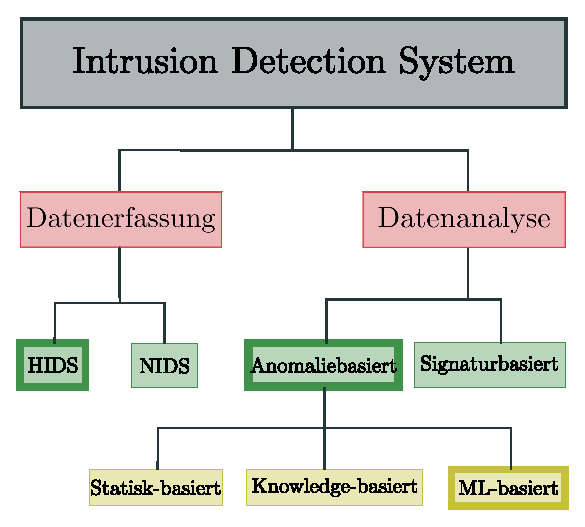
\includegraphics[width=1\textwidth]{images/Illustrationen/IDS/IDSOverview}
            \caption{Einordnung des verwendeten IDS (breiter markiert).}
            \label{fig:IDSOverview}
        \end{figure}

    \section{System Calls}
    \label{sec:syscalls}
        Jegliche Programme die auf einem Rechner mit einem Betriebssystem laufen müssen mit diesem interagieren um Veränderungen am System vornehmen zu können.
        Diese Interaktion findet in Form von \textit{System Calls} \marginpar{zu dt. Systemaufrufe} statt.
        Zu ihnen gehören zum Beispiel die in \autoref{tab:syscall} beschiebenen System Calls.

        \begin{table}[H]
            \small
            \label{tab:syscall}
            \centering
            \begin{tabular}{c||p{6cm}|p{3cm}|p{3cm}}
                \hline
                \rowcolor{Gray!36}
                \multicolumn{4}{c}{System Calls}\\
                \hline
                Name & Beschreibung & Argumente & Rückgabewerte\\
                \hline
                \hline
                \rowcolor{Gray!16}
                %open& Öffnet die von \textit{pathname} spezifizierte File. Falls diese nicht existiert kann sie mit dem Zusatz \textit{O_CREAT} automatisch erstellt werden & path, asdklfjs, slddk\\
                open& Öffnet die in \textit{path} spezifizierte File und gibt einen \textit{file descriptor} zurück.& \textit{path}, \textit{flags}, \textit{mode} & kp\\
                write& Schreibt bis zu \textit{count} Bytes aus dem Buffer (ab Stelle \textit{buf}) in die File, welche über den \textit{file descriptor}$fd$ definiert wird. & $fd$, $*buf$, \textit{count} & kp\\
                \hline
            \end{tabular}
            \caption{Beschreibung ausgewählter System Calls}
        \end{table}

        Generell werden System Calls verwendet um vom Betriebssystem zur Verfügung gestellte Funktionalitäten auszuführen.
        Das Betriebssystem, oder noch genauer der \textit{Kernel} \marginpar{zu dt. Betriebssystemkern} des Betriebssystems stellt verschiedene Services bereit welche von Programmen genutzt werden können. 
        Die System Calls stellen dabei die Kommunikation zwischen Kernel und Programmen dar.
        Mögliche Services sind unter anderem Zugriffe auf Hardware aber auch das Erstellen und Ausführen von Prozessen.
        Üblicherweise können System Calls nur von Nutzerprozessen ausgelöst werden, welche eine eingeschränkte Berechtigung besitzen.
        Wie in \autoref{tab:syscall} ebenfalls beschrieben besitzen System Calls auch Argumente die beim Aufrufen mitgegeben werden können sowie einen Rückgabewert.

        Auch ein möglicher Angreifer muss um Schaden anzurichten also an den System Calls in irgendeiner Form eine Veränderung vornehmen.
        Entweder kann die Abfolge, also die Sequenz von System Calls verändert werden, z.B. es werden neue Funktionen aufgerufen, welche wiederum andere System Calls aufrufen,
        oder es werden die Argumente der System Calls verändert.
        So könnte zum Beispiel anstatt auf den Pfad \glqq /tmp/some/file\grqq \ auf \glqq /etc/passwd\grqq \ zugegriffen werden. 
        Viele verschiedene IDS Ansätze betrachten lediglich die Sequenz von System Calls und missachten die in den Argumenten enthaltene Informationen.
        Auch wenn diese Ansätze teilweise sehr erfolgreich sind, lassen sie den Angreifenden einen Spielraum.
        %Denn eine Veränderung der System Call Sequenz kann auch verhindert werden.
        Verschiedene Arbeiten~\cite{Syscallseqexploit1},~\cite{Syscallseqexploit2},~\cite{Syscallseqexploit3} zeigen, wie dieser Spielraum ausgenutzt werden kann um unerkannt Angriffe durchzuführen. 
        Tan et al. \cite{Syscallseqexploit3} erreichen dies durch die Veränderung eines zuvor von der IDS erkannten Angriffes.
        Sie beschreiben, wie dem IDS fremde System Call Sequenzen derart Verändert werden können, dass sie als normal eingestuft werden.
        Dabei werden die fremden Sequenzen auseinander gezogen und mit bekannten Sequenzen aufgefüllt.\marginpar{Verwendeter Algorithmus: STIDE~\cite{FORREST}} 
        Ein weiterer Ansatz versucht lediglich die System Call Argumente zu verändern, ohne dabei die Sequenz zu beeinflussen~\cite{Syscallseqexploit1}.
        Doch diese Beispiele zeigen auch, dass wenigstens ein Faktor, also Sequenz oder Argumente, verändert werden muss, um das Systemverhalten abzuwandeln.
        Welche dieser Argumente und wie diese genutzt werden können um die Anomalieerkennung zu verbessern soll in Kapitel~\ref{sec:args} untersucht werden.
        Im dem nachfolgenden Kapitel wird nun auf verschiedene Datensätze, welche System Call Sequenzen enthalten, eingegangen.

    \section{Datensatz}
    \label{sec:Datensatz}
        Seit 1998 einer der ersten System Call Datensätze für HIDS veröffentlicht wurde~\cite{DARPA},
        kamen verschiedene Datensätze hinzu.
        Auf diese wird in den kommenden Abschnitten kurz eingegangen.
        Dabei soll auch auf die Nutzbarkeit und die entstehenden Problematiken dieser für die HIDS über System Calls eingegangen werden.

        \paragraph{KDD}
            Der unter anderen von der \textit{Defence Advanced Research Project Agency}, kurz DARPA, erstellte Datensatz KDD-99~\cite{DARPA}
            steht auf Grund verschiedener Unzulänglichkeiten schon länger in der Kritik~\cite{KDD}~\cite{KDD2}~\cite{UNM}.
            Zum einen ist der Datensatz veraltet (1999) und zum anderen gibt es Diskrepanzen in den Daten, wie unter anderem von Vegard Engen beschrieben wird~\cite{KDD}.
        \paragraph{UNM}
            Auch dieser Datensatz~\cite{UNM} ist veraltet (1999) und kommt für eine weitere Betrachtung nicht in Frage,
            da zusätzlich auch weitere Kontextinformationen wie Thread IDs fehlen~\cite{UNMcritic}
        \paragraph{ADFA-LD}
            Der ADFA-LD Datensatz wurde von Hu et al.~\cite{UNMcritic} im Jahre 2013 erstellt und ist damit wesentlich aktueller als die zuvor genannten.
            Aufzeichnungen wurden auf dem Betriebssystem Ubuntu 11.04 durchgeführt, allerdings wurden diese nicht gut dokumentiert was ein bearbeiten erschwert~\cite{ADFA-LDcritic}.
            Erschwerend kommt hinzu, dass lediglich Sequenzen von System Call IDs aufgezeichnet wurden und damit keine Metadaten beinhalten.
        \paragraph{NIGDS-DS}
            Der 2017 erstellte Datensatz NIGDS-DS beinhaltet Thread Informationen, aber auch hier fehlen weitere Daten wie zum Beispiel System Call Argumente.
            Ein weiteres großes Problem liegt in der Ungenauigkeit der Zeitstempel, welche nur auf die Sekunde genau sind.
            Des Weiteren ergeben sich Schwierigkeiten in der Zuordnung von der beschriebenen Event ID und den Zeitstempeln.
        \paragraph{LID-DS}
            2019 veröffentlichten Grimmer et al.~\cite{LIDDS} das \textit{Leipzig Intrusion Detection-Data Set} (LID-DS).
            Sie erkannten, dass die bisherigen Datensätze entweder veraltet oder nicht ausreichend waren um zum Beispiel Thread IDs oder System Call Argumente für ein IDS zu verwenden.
            Im folgenden soll eine Beispieldatei betrachtet werden.

            \begin{table}[h]
                \tiny
                \centering
                \begin{tabular}{p{1.1cm}|p{1.1cm}|p{0.3cm}|p{0.4cm}|p{0.6cm}|p{0.6cm}|p{0.8cm}|p{0.6cm}|p{1cm}}
                    \rowcolor{Gray!36}
                    \hline
                    \multicolumn{9}{c}{System Call}\\
                    \hline
                    event number & event time & cpu & user uid & process name & thread id & event direction & event type & event arguments\\
                    \hline
                    \hline
                    \rowcolor{Gray!16}
                    4012 & $10:18:20.1231231231$ & 0 & 33 & apache2 & 1425 & > & writev & $fd=12(<4t>172.131.12.1:123\rightarrow172.13.231.2:123)size=2392$ \\
                \end{tabular}
                \caption{Ausschnitt aus LID-DS~\cite{LIDDS}}
                \label{tab:syscallfile}
            \end{table}

            \begin{table}[h]
                \small
                \centering
                \begin{tabular}{p{3cm}|p{6.5cm}}
                    \rowcolor{Gray!36}
                    \hline
                    \multicolumn{2}{c}{Scenarien}\\
                    \hline
                    Name & Beschreibung \\
                    \rowcolor{Gray!16}
                    \hline
                    \hline
                    Bruteforce\_CWE-307 & Ungeeignete Einschränkung von übermäßigen Authentifizierungs Versuche \\
                    \hline
                    CVE-2012-2122 & Umgehung von MySQL Authentifizierung\\
                    \rowcolor{Gray!16}
                    \hline
                    CVE-2014-0160 & Heartbleed: Schwachstelle in OpenSSL\\
                    \hline
                    CVE-2017-7529 & Nginx Integer Overflow \\
                    \rowcolor{Gray!16}
                    \hline
                    CVE-2018-3760 & Sprockets Datenleck Schwachstelle \\
                    \hline
                    CVE-2019-5418 & Rails Fileinhalt Offenlegung \\
                    \rowcolor{Gray!16}
                    \hline
                    EPS\_CWE-434 & EPS file upload: uneingeschränkter Upload von gefährlichen Dateitypen  \\
                    \hline
                    PHP\_CWE-434 & PHP file upload: uneingeschränkter Upload von gefährlichen Dateitypen  \\
                    \rowcolor{Gray!16}
                    \hline
                    SQL Injection & SQL Injection mit sqlmap\\
                    \hline
                    ZipSlip & blablabla \\
                \end{tabular}
                \caption{Ausschnitt aus LID-DS~\cite{LIDDS}}
                \label{tab:scenarien}
            \end{table}
            Der Datensatz umfasst zehn verschiedene Angriffsscenarien, dargestellt in Tabelle~\ref{tab:scenarien}.
            Jede Aufzeichnung eines Scenarios enthält ca. 1000 Files welche jeweils ca. 60sec Aufnahmen beinhalten.
            Dies führt zu insgesamt ungefähr 10h Trainingsdaten pro Scenario.

            In den Testdaten sind \textit{malicious} \marginpar{zu dt.\ schädlich} Files beinhaltet, welche eine Information über den Angriffszeitpunkt liefert. 
            Jedoch gibt es bei einer malicious File im Gegensatz zu den normalen Files  vier mögliche Zuordnungen.
            Befindet sich der Anomaliescore unter dem Schwellwert kann von einem \textit{True Negative} eingestuft werden.
            Also es wurde korrekter weise kein Alarm vorhergesagt.
            Befindet sich der Anomaliescore vor dem Angriffszeitpunkt über dem Schwellwert liegt ein \textit{False Positive} vor.
            Es wurde ein Alarm gemeldet an einer Stelle an dem kein Angriff stattfand.
            Nach dem angegebenen Angriffszeitpunkt wird es allerdings schwieriger.
            Denn liegt der Anomaliescore nach dem Angriffszeitpunkt über dem Schwellwert, wird von einem \textit{True Positive}, also einem korrektem Alarm ausgegangen.
            Jedoch könnte da der Angriff schon vorbei sein, oder gar noch nicht gestartet sein.
            Es können nach dem Angriffszeitpunkt auch \textit{False Positive} oder \textit{False Negative} geben, welche allerdings nicht als solche erkannt werden können.
            Wie sich das auf die Auswertung der Ergebnisse auswirkt wird in Kapitel~\ref{sec:metrik} beleuchtet.

            Nachdem nun verschiedene allgemeine Ansätze zur Erkennung von schädlichem Verhalten eines Systems und mögliche Datensätze zur Auswertung untersucht wurden,
            soll im Folgenden die Frage geklärt werden, wie Muster mit Hilfe von künstlichen neuronalen Netzen in einem Datensatz erkannt werden können.

    \section{Künstliche neuronale Netze}
    \label{sec:KNN}        
        Das Nutzen von bestehenden und in der Natur vorkommenden Strukturen und Prozessen kommt in verschiedenen Forschungsbereichen zum Einsatz.
        In direkter Umsetzung von zum Beispiel der Struktur von Geckofüßen unter anderem für die Raumfahrt~\cite{GECKO}.%, oder auch zur Verringerung des Luftwiderstandes mit der Adaption von Placoidschuppen der Haie \cite{SHARK}.
        Auch Prozesse welche in der Natur beobachtbar sind werden verucht zu adaptieren, dazu zählen zum Beispiel Ameisenalgorithmen~\cite{ANT}.
        Ein in den letzten Jahren immer weiter verbreiteter Ansatz in der elektronischen Datenverarbeitung ist die Verwendung von künstlichen neuronalen Netzen.
        Dieser versucht sich die Struktur von Gehirnen anzueignen.
        Man verspricht sich mit dem Einsatz von künstlichen neuronalen Netzen, welche eine Varietät an verschiedenen Architekturen beinhalten, diverse Optimierungsprobleme zu lösen.
        %In dieser Arbeit wird der Einsatz von neuronalen Netzen zur \textit{Time Series Prediction} (zu dt. Vorhersagen von Zeitreihen) untersucht.
        Zu aktuellen Beispielen zählen dabei auch Vorhersagen die im Zusammenhang mit der Verbreitung des COVID-19 Virus stehen~\cite{COVID1}~\cite{COVID2}~\cite{COVID3}.
        %Für die \textit{Time Series Prediction} sind verschieden Architekturen von neuronalen Netzen weit verbreitet \cite{BENIDIS2020}.
        
        Algorithmen in welchen neuronale Netze zum Einsatz kommen bestehen generell aus zwei Phasen. 
        In der ersten Phase, der Trainingsphase, werden vordefinierte Trainingsdaten in das Netz gegeben.
        Dieses versucht Merkmale in den Daten zu ermitteln, mit welchen dann in der Testphase Voraussagen gemacht werden können.
        Dabei haben sich spezialisierte Herangehensweisen entwickelt, wie zum Beispiel die \textit{Convolutional Neural Nets} (CNN) für die Bilderkennung. 
        Für sequentielle Daten wie Audio, Text und Video, bei welchen eine zeitliche Komponente entscheidend ist, eignen sich vor allem die \textit{Recurrent Neural Nets} (RNN).
        Da in dieser Arbeit sequentielle Daten betrachtet werden, die sequentielle Abfolge von System Calls, soll im Folgenden nur auf die RNNs und besondere Abwandlungen dieser eingegangen werden.
        
        % überarbeiten
        %unterteilung verschiedener Netze und einordnung von rnns und lstmnn
        
        %Neuronale Netze bestehen aus verschiedenen Ebenen von Knoten (auch Neuronen genannt), die miteinander verbunden sind.
        %Die Neuronen erhalten Eingangssignale und falls diese eine bestimmte Bedingung erfüllen (z.B. Schwellwertüberschreitung) wird das Ausgangssignal des Neurons verändert.
        %Wird die Bedingung nicht erfüllt, sendet das Neuron ein Signal, welches die nachfolgenden Neuronen nicht beeinflusst. Der schematische Aufbau wird in Abbildung \ref{fig:Neuron} gezeigt.
%
        \subsection{Rekurrente neuronale Netze}
        \label{sec:RNN}
            Der entscheidende Unterschied von RNNs zu herkömmlichen neuronalen Netzen ist,
            dass der Ausgang eines Knotens auf einer \textit{Layer} \marginpar{zu dt. Ebene} mit einer vorherigen oder derselben Layer verbunden ist.
            Ist dies der Fall spricht man von einem \textit{Feedback} oder \textit{Recurrent Neural Network}, sonst von einem \textit{Feedforward Neural Network}. 
            Mit Knoten, die eine extra Verbindung zu sich selbst haben, können frühere Eingaben Einfluss auf die Behandlung der nächsten Eingabe haben.
            Der einzelne Knoten merkt sich seine Ausgabe, welche im nächsten Zeitschritt als weiteres Eingabesignal dient.
            Dadurch wird es ermöglicht auch zeitlich abhängige Sequenzen zu erlernen, da die Signalverarbeitung der RNNs auch vorherige Geschehnisse mit einbezieht.
            Im Gegensatz dazu steht zum Beispiel die Bilderkennung, bei welchem das vorherige Bild keinen Einfluss auf die Einschätzung des aktuellen Bildes hat.
            Dieser Zusammenhang lässt sich in der folgenden Gleichung darstellen.
            \begin{equation}
                \begin{split}
                    h_t &= \sigma \left(W_{h}h_{t-1} + W_{x}x_{t} + b\right)\\
                    y_t &= h_t
                \end{split}
            \end{equation}
            Dabei beschreiben $x_t$, $h_t$ und $y_t$ den Eingang des Neurons, die rekurrente Information und den Ausgang des RNN\@.
            $W_h$ und  $W_x$ beschreiben die Gewichte und $b$ den Bias.
            Ein einzelner Knoten wird ohne die Gewichte in Abbildung~\ref{fig:RNN} dargestellt,
            sowie in Abbildung~\ref{fig:RNN_enroled} in einer alternativen Darstellung, wie sich dieser Knoten über $t$ Zeitpunkte verhält.
            Dabei werden für die Übersichtlichkeit Gewichte sowie der Bias nicht dargestellt.
                \begin{figure}[h]
                    \centering
                    \includegraphics[width=0.8\textwidth]{images/Illustrationen/RNN_simple}
                    \caption{Darstellung einer RNN Zelle}
                    \label{fig:RNN}
                \end{figure}
                \begin{figure}[h]
                    \centering
                    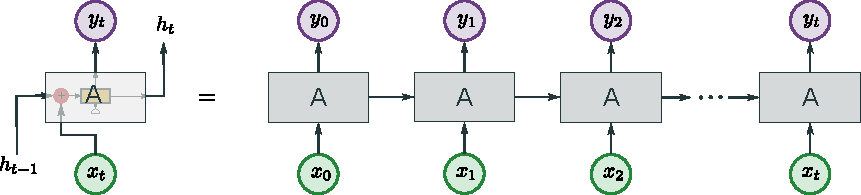
\includegraphics[width=1\textwidth]{images/Illustrationen/RNN_enrolled}
                    \caption{Darstellung einer \glqq ausgerollten\grqq \ und vereinfachten RNN Zelle}
                    \label{fig:RNN_enroled}
                \end{figure}
            Doch auch die RNNs haben ein Problem bei Merkmalen, die sich über einen längeren Zeitraum strecken.
            Denn dabei kommt es häufig vor, dass durch die Back Propagation die berechneten Gradienten entweder verschwindend klein, oder sehr groß werden.
            Gerade bei Abhängigkeiten über einen größeren zeitlichen Abstand tendieren die Fehlersignale,
            die durch die Back Propagation durch das Netz gegeben werden, zu geringe Gewichtsänderungen auszulösen.
            Traditionelle Aktivierungsfunktionen wie die hyperbolische Tangensfunktion haben Gradienten im Bereich $(-1,1)$ oder $[0,1)$ und Backpropagation berechnet Gradienten durch die Kettenregel.
            Dies hat den Effekt, dass n dieser kleinen Zahlen multipliziert werden, um die Gradienten der \glqq vorderen\grqq \ Schichten in einem n-Schichten-Netzwerk zu berechnen, was bedeutet, dass der Gradient (Fehlersignal) exponentiell mit n abnimmt und die vorderen Schichten sehr langsam trainieren.
            Die von Sepp Hochreiter erstmals erwähnte \textit{Long Short-Term Memory} (LSTM) Zellen ermöglichen durch verbesserte Fehlerkorrektur stabilere Lernergebnisse sowie auch das Lernen von Mustern mit noch größeren zeitlichen Abständen.~\cite{HOCHREITER1998}

            Diese Sonderform der RNNs, die auch in dieser Arbeit verwendet werden, sollen deshalb genauer untersucht werden.
            %% TODO Batch Normalisation \cite{LSTMbatchnorm}
   	
        \subsection{Long Short-Term Memory} 
            Hauptziel der LSTMs ist es, das Lernen der zeitlich abhängigen Muster zu verbessern.
            Entscheident dafür ist die Einschätzung welche zuvor gesehenen Informationen für die aktuelle Eingabe relevant sein könnten.
            
            \begin{figure}[h]
                \centering
                \includegraphics[width=0.8\textwidth]{images/Illustrationen/LSTM}
                \caption{Schematische Darstellung eines Knotens in einem LSTM NN, mit Input, Output und Forget Gate (inspiriert von \cite{OLAH2015}).}
                \label{fig:LSTM}
            \end{figure}

            Und um zu erlernen welche früheren Ausgaben für die Ermittlung nächster Datenpunkte entscheident sind, wird an jedem Knoten eine \textit{Memory Cell} \marginpar{zu dt. Gedächtniszelle} angebracht, zu sehen ist diese Erweiterung in Abbildung~\ref{fig:LSTM}.
            Sie ist mit sich selbst verbunden, kennt also die vorherigen Ausgaben und gibt den Zellstatus an.
            Mit Hilfe dieser Information soll eine Abhängigkeit auch über einen längeren Zeitraum gefunden werden.
            Der Zellstatus $C_{t-1}$ zum Zeitpunkt $t-1$ hat im nächsten Zeitschritt $t$ einen Einfluss auf den Zellstatus $C_{t}$ und somit auch auf die Ausgabe $y_t$.
            Die Weitergabe des Status wird in Abbildung~\ref{fig:LSTM_Status} dargestellt.

                \begin{figure}[h]
                    \centering
                    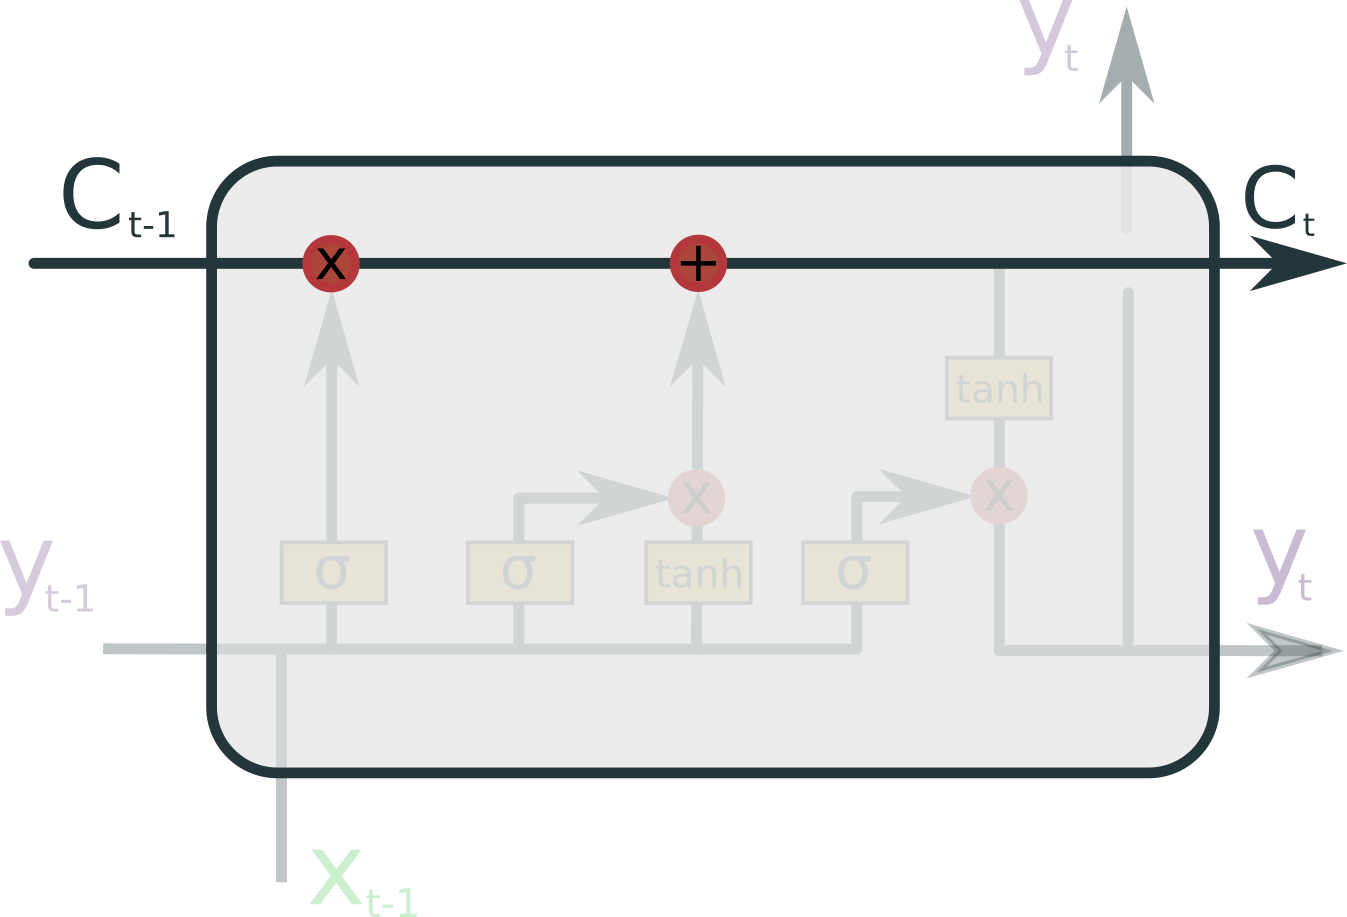
\includegraphics[width=0.5\textwidth]{images/Illustrationen/LSTM_MC}
                    \caption{Weitergabe des Zellstatus innerhalb eines Knotens (inspiriert von \cite{OLAH2015}).}
                    \label{fig:LSTM_Status}
                \end{figure}
                
                Einfluss auf den Zellstatus haben zwei verschiedene \textit{Gates} \marginpar{zu dt. Gatter/Tore}.
            Im ersten Schritt wird entschieden, welche Information aus dem vorherigen Zeitschritt keinen Einfluss mehr auf den Zellstatus haben sollen.
            Dies wird mit dem \textit{Forget Gate} umgesetzt und ist in Abbildung~\ref{fig:LSTM_Forget} zu sehen und kann analog zur RNN Zelle folgendermaßen hergeleitet werden.

            \begin{equation}
                f_t = \sigma\left(W_{fh}h_{t-1} + W_{fx}x_t + b_f\right)
            \end{equation}

            $W_{fh}$ und $W_{fx}$ beschreiben die Gewichte $b_f$ den Bias des \textit{Forget Gate}.
            Es wird also die vorherige Eingabe $h_{t-1}$ sowie die aktuelle Eingabe $x_t$ gewichtet und mit Bias an die Aktivierungsfunktion $\sigma$ übergeben.
            Damit sollen Informationen aus dem Speicher, die keinen Einfluss mehr haben sollen, entfernt werden.
            In dem Sprachbeispiel könnte das Genus (\textit{grammatikalisches Geschlecht}) gespeichert werden, um so eine grammatikalisch korrekte Vorhersage zu machen.
            Kommt nun allerdings ein neues Pronomen in der Eingabe $x_t$, sollte das bisher gespeicherte Genus keinen Einfluss mehr haben.
            
                \begin{figure}[h]
                    \centering
                    \includegraphics[width=0.5\textwidth]{images/Illustrationen/LSTM_FG}
                    \caption{Einfluss des Forget Gates auf den Zellstatus (inspiriert von \cite{OLAH2015}).}
                    \label{fig:LSTM_Forget}
                \end{figure}
                
            Das \textit{Input Gate} soll im nächsten Schritt angeben, welche neuen Informationen in den Zellstatus $C_t$ aufgenommen werden.
            Dies erfolgt in zwei Schritten, zunächst wird mit $i_t$ ermittelt, welche Information geupdated werden soll.

            \begin{equation}
                \begin{split}
                    i_t &= \sigma\left(W_{ih}h_{t-1} + W_{ix}x_t + b_i\right), \\
                    \tilde{C}_t &= tanh\left(W_{\tilde{C}h}h_{t-1} + W_{\tilde{C}x}x_t + b_{\tilde{C}}\right),\\
                \end{split}
            \end{equation}

            Im Vektor $\tilde{C}$ sind mögliche Kandidaten enthalten (wie z.B. das Genus), welcher den zuvor vergessenen Wert ersetzen soll (vgl. Abbildung~\ref{fig:LSTM_Input}).
            Der gesamte Zellstatus $C_t$ wird dann zusammen mit Werten aus dem \textit{Forget Get} verrechnet.

            \begin{equation}
                \begin{split}
                    C_t &=f_t\times C_{t-1} + i_t\times \tilde{C}_t, \\
                \end{split}
            \end{equation}

                \begin{figure}[h]
                    \centering
                    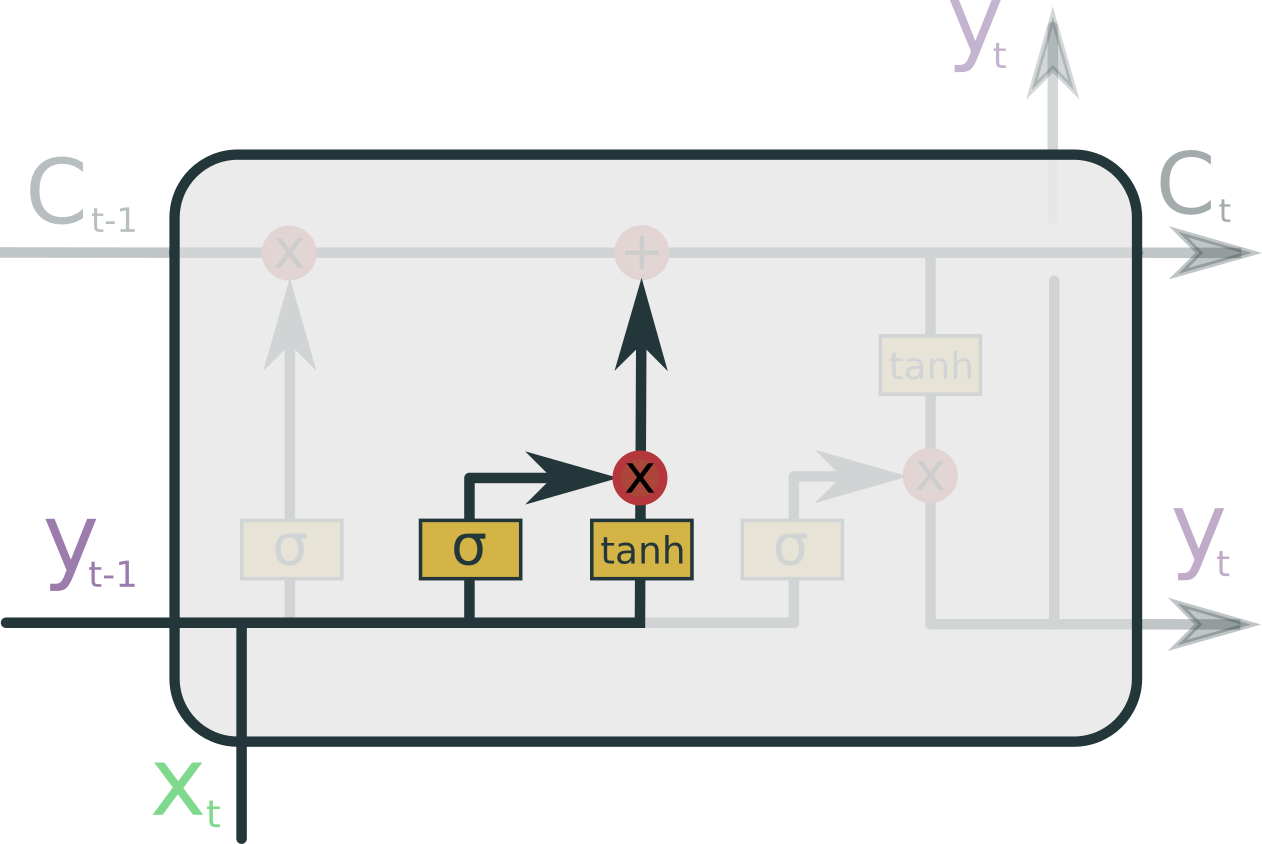
\includegraphics[width=0.5\textwidth]{images/Illustrationen/LSTM_IG}
                    \caption{Einfluss des Input Gates auf den Zellstatus (inspiriert von \cite{OLAH2015}).}
                    \label{fig:LSTM_Input}
                \end{figure}
            
            Wie der Zellstatus $C_t$ nun die Ausgabe beeinflusst, wird über das \textit{Output Gate} geregelt (siehe Abbildung~\ref{fig:LSTM_Output}).
            \begin{equation}
                \begin{split}
                    o_t &= \sigma\left(W_{oh}h_{t-1} + W_{ox}x_t + b_o \right), \\
                    h_t &= o_ttanh\left(c_t\right)
                \end{split}
            \end{equation}
            Dies soll in unserem Sprachbeispiel entscheiden, ob die Information des Genus für die Vorhersage des nächsten Wortes eine Rolle spielt. \cite{GERS2000} \cite{OLAH2015}

                \begin{figure}[h]
                    \centering
                    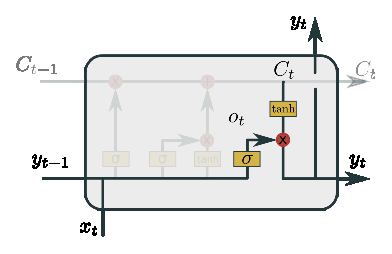
\includegraphics[width=0.5\textwidth]{images/Illustrationen/LSTM_OG}
                    \caption{Das Output Gate regelt den Einfluss des Zellstatus auf die Ausgabe des Neurons (inspiriert von \cite{OLAH2015}).}
                    \label{fig:LSTM_Output}
                \end{figure}
            
            Die verschiedenen Gates können so als ein weiteres kleines NN in jedem Knoten der LSTM Netze betrachtet werden, welche einen zeitlichen Zusammenhang besser erkennen sollen.
            Gesamt lässt sich eine LSTM Zelle mit den folgenden Formeln beschreiben:
            \begin{equation}
                \begin{split}
                    f_t &= \sigma\left(W_{fh}h_{t-1} + W_{fx}x_t + b_f\right) \\
                    i_t &= \sigma\left(W_{ih}h_{t-1} + W_{ix}x_t + b_i\right), \\
                    \tilde{C}_t &= tanh\left(W_{\tilde{C}h}h_{t-1} + W_{\tilde{C}x}x_t + b_{\tilde{C}}\right),\\
                    C_t &=f_t\times C_{t-1} + i_t\times \tilde{C}_t, \\
                    o_t &= \sigma\left(W_{oh}h_{t-1} + W_{ox}x_t + b_o \right), \\
                    h_t &= o_ttanh\left(c_t\right) \\
                    y_t &= h_t
                \end{split}
            \end{equation}



%*****************************************
\chapter{Verwandte Arbeiten}\label{ch:verwandte_arbeiten}
%*****************************************

Die Forschungsfrage mit der sich diese Arbeit beschäftigt kann wie in~\autoref{sec:Forschungsfrage} beschrieben weiter unterteilt werden.
Zum einen soll untersucht werden inwiefern \ac{LSTM} neuronale Netze in anomaliebasierten \ac{HIDS} Vorteile bringen können.
Und zum anderen wie durch die Anreicherung der Sequenzen von System Calls, durch weitere Informationen neben dem Namen des System Calls, die \ac{FP}-Rate sowie die \ac{DR} verbessert werden kann.
Um den Überblick über die verwandten Arbeiten zu bewahren sind diese im Folgenden untergliedert.
Zunächst sollen Grundlagen der Anomalieerkennung und erste Ansätze der Anomalieerkennung mit System Calls aufgeführt werden, auf welchen diese Arbeit indirekt fußt.
Im nächsten Schritt werden dann Arbeiten betrachtet, welche sich auf die Argumente der System Calls konzentrieren.
Abschließend werden Arbeiten untersucht welche sich speziell mit dem Transfer von \ac{NLP} Verfahren in die anomaliebasierte \ac{HIDS} auseinandersetzen.
Dazu zählen auch Ansätze der mit \ac{LSTM} Netzwerken.

\section{Grundlagen Anomaliedetektion}

    % Die Anomaliedetektion findet nicht nur in der IT-Sicherheit ihren Einsatz und kann .
    % Dazu gehören die Erkennung von Betrug, unter anderem bei Kreditkarten~\cite{CREDITBOLTON2001}, das Aufdecken von Unregelmäßigkeiten in medizinischen und Gesundheitsdaten~\cite{MEDIZINHORN2001} oder Schadenserkennung in der Industrie~\cite{INDUSTRIEBASU2007}.
    Die Anfänge der Anomalieerkennug werden von~\cite{ANOMALYBOOKKISHAN2017} auf die Arbeit von Grubbs~\cite{ANOMALYDEFINITION1969} zurückgeführt, in welcher sogenannte Ausreißer in Sample-Daten gefunden und entfernt werden sollen.
    Hingegen berufen sich~\cite{ANOMALYSURVEY} bei den Anfängen der Anomalieerkennung auf eine Arbeit aus dem~\textit{Dublin Philosophical Magazine of Journal and Science} von 1887~\cite{ANOMALYDEFINITION1887}.
    Dort werden \textit{discordant observations}\marginpar{zu dt.\ nicht stimmige Beobachtung} anhand einer abweichenden gesetzmäßigen Frequenz isoliert. 
    Speziell im Kontext der Angriffserkennung wird wie in~\autoref{sec:Datenerfassung} beschrieben die Anomalieerkennung in \ac{NIDS} und \ac{HIDS} eingeteilt.
    Da es wie in der Anomalieerkennung in diesen Bereichen eine große Anzahl an Arbeiten und auch Übersichtsarbeiten gibt~\cite{ANOMALYSURVEY, ANOMALYSURVEY2, ANOMALYSURVEY3}, soll im Folgenden nur auf bestehende Arbeiten im Bereich der \ac{HIDS} eingegangen werden, welche speziell System Calls verwenden.

\section{Anomaliebasierte HIDS mit System Calls}

    Zunächst soll im Folgenden \ac{HIDS} betrachtet werden die explizit nur die Sequenzen der System Call Namen betrachten und alle weiteren Informationen nicht beachten.

    \paragraph{Ohne Betrachtung der System Call Argumente}
        Bereits 1996 stellten Stephanie Forrest et al.~\cite{FORREST} die erste Arbeit vor in welcher sie mit ihrem \ac{TIDE} Algorithmus Anomalien in System Call Daten ermitteln.
        Dabei wird anhand einer Datenbank gültiger System Call Paare, \textit{lookahead pairs}, ermittelt ob eine System Call Sequenz eine Anomalie darstellt.

        In einer späteren Arbeit erweitern sie diesen Ansatz, indem sie die Datenbank mit zusammenhängende Sequenzen von System Calls befüllen.
        Kommt eine Sequenz nicht in der Datenbank vor wird diese als Anomalie eingestuft.
        So wird \ac{TIDE} zu \ac{STIDE}.~\cite{STIDE}

        Ein anderen Ansatz wählten 1997 Lee et al.~\cite{LEE1997}, wobei sie sich auch auf die Pionierarbeit von~\cite{FORREST} berufen.
        Sie versuchen mit dem \ac{ML}-Programm \ac{RIPPER} Regeln aus den System Call Daten abzuleiten.
        Im Gegensatz zu~\cite{FORREST} befinden sich bei diesem Ansatz normale sowie anormale Sequenzen in den Trainingsdaten.

        1999 untersuchten Warrender et al.~\cite{STIDE_Alternatives} wie verschiedene Algorithmen auf System Call Daten abschneiden.
        Dazu gehören die bereits erwähnten Verfahren \ac{TIDE}, \ac{STIDE}, \ac{RIPPER}, sowie ein \ac{HMM}.
        Dabei schienen alle Verfahren erfolgreich wobei das \ac{HMM} als sehr rechenintensiv hervorgehoben wird.
        Speziell interessant an dieser Arbeit ist auch die Verwendung von n-grammen aus der Textverarbeitung.
        Ein n-gramm ist eine zusammenhängende Folge von n Elementen aus einer gegebenen Eingabe.
        Oft wird diese Art der Vorverarbeitung bei Datenstreams eingesetzt.
 
        % Auch in moderneren Arbeiten werden die Abfolge von System Calls beziehungsweise speziell nur die Funktionsnamen verwendet.
        Auch aktuellere Arbeiten befassen sich mit der Anomalieerkennung mit System Calls und verwenden dabei speziell nur die Namen von System Calls, ohne die Einbindung der System Call Argumente.
    
        2005 betrachten Kang et al.~\cite{FREQUENCY2} nicht die Sequenzen sondern die Frequenzen der auftretenden System Calls.
        Dabei zählen sie das Vorkommen von System Calls in einem bestimmten Zeitfenster und verwenden diese sogenannten \textit{bag of system calls}\marginpar{zu dt. Bündel von Systemaufrufen} für ihre Beschreibung des Normalverhaltens.
        Ähnlich zu~\cite{FORREST} und~\cite{STIDE} bauen sie mit diesen Bündelungen eine Datenbank für das Normalverhalten auf.

        2013 stellen Murtaza et al.~\cite{SYSTEM_STATES} System Calls als Zustände von Kernelmodulen dar, indem sie System Calls einem bestimmten Modul zuschreiben.
        Dazu gehört zum Beispiel das Modul \textit{File System} mit den System Calls \textit{read} \textit{write} etc., oder auch \textit{Architecture}, \textit{Memory Management}.
        Der Wahrscheinlichkeiten für das Auftreten von Zustandssequenzen wird dann zur Identifizierung von Anomalien genutzt.

        2018 interpretieren Grimmer et al.~\cite{SYSCALL_GRAPHS} System Call Sequenzen als einen sogenannten \textit{System Call Graph}.
        Dabei werden wie in~\cite{STIDE_Alternatives} n-gramme verwendet.
        Die n-gramme stellen einen Knoten dar und der Übergang eines n-gramms zu einem weiteren wird mit einer gerichteten Kante dargestellt.
        Zusammen mit den Häufigkeiten des Auftretens eines Überganges und dem Ausgangsgrad eines Knotens ergeben sich dann die Übergangswahrscheinlichkeiten für alle Knoten.
        Der Anomaliescore eines Fensters von n-grammen aus den Testdaten wird dann anhand der Übergangswahrscheinlichkeiten aus dem im Training aufgebauten Graphen abgelesen.

        % (2015) Einsatz in Linux Containern~\cite{FREQUENCY1} oder (2018) in Cloud Lösungen~\cite{VM}

    Doch es gibt auch mehrere Arbeiten die Schwachstellen der Angriffserkennung mittels Sequenzen von System Calls aufzeigen.
    % Zumindest sofern nur die Sequenz der System Calls betrachtet wird.
    In~\cite{Syscallseqexploit1} werden verschieden Methoden untersucht mit welchen Angriffe nicht durch das IDS von~\cite{FORREST2000}\marginpar{beruht auf \ac{STIDE}~\cite{STIDE}} erkannt wurden.
    Bei ihren theoretischen Ansätzen berufen sie sich unter anderem auf das Abändern von System Call Argumenten, ohne dabei auf die Sequenz der System Calls einfluss zu nehmen.
    Und~\cite{Syscallseqexploit3} untersuchen speziell die von~\cite{FORREST} ins Spiel gebrachte Fensterlänge von $6$ für den \ac{STIDE} Algorithmus.
    Dabei umgehen sie die Angriffserkennung in dem sie die Angriffssequenzen auseinanderziehen und mit Normalsequenzen auffüllen.


    \paragraph{Mit Betrachtung der System Call Argumente}\label{sec:related_sys_arg}

        Dies zeigt, dass es sinnvoll sein kann auch noch weitere Informationen welche in den System Calls enthalten sind einzubinden.
        Seien es Metadaten wie die Thread Information der System Calls, oder auch die eigentlichen Argumente der Aufrufe.
        Inwiefern diese zusätzlichen Informationen bereits in der Literatur verwendet wurde soll nun behandelt werden.

        2003 wählen Kruegel et al.~\cite{ARGUMENTS} einen zu den bisherigen Arbeiten konträren Weg.
        Sie missachten die Sequenz und betrachten nur die Rückgabewerte und Argumente der System Calls.
        Sie erstellen in der Trainingsphase für jeden System Call verschiedene Modelle, welche in der Testphase die Wahrscheinlichkeit eines anormalen Verhaltens bestimmen.
        Speziell nutzen sie aber auch zuvor gesammelte Informationen über mögliche Angriffe für die Erstellung der Modelle.
        Spannend dabei sind vor allem die vorgestellten Modelle, welche nun im Folgenden genauer beschrieben werden.

        \textit{String Length}: Die Annahme dieses Features besteht darin, dass sich bei einem Angriff die String-Länge der Argumente signifikant ändert.
        Dafür wird in der Trainingsphase versucht die Verteilung der String-Längen zu approximieren.S
        In der Testphase wird dann die Wahrscheinlichkeit dafür, dass die aktuelle String-Länge aus der Verteilung stammt mit der \textit{Tschebyschaffschen Ungleichheit} berechnet.
        
        \textit{String Character Distribution}: Hier wird angenommen, dass es unter legitimen System Calls Ähnlichkeiten unter den Frequenzen der auftretenden Zeichen eines Strings gibt.
        In der Trainingsphase wird für jedes gesehene Argument die Zeichenverteilung hinterlegt.
        Ähnlich zu der String-Länge zuvor wird in der Testphase nun überprüft mit welcher Wahrscheinlichkeit die aktuelle Zeichenverteilung aus der gespeicherten Verteilung gezogen werden kann.

        \textit{Structural Inference:} Da Angriffe laut Kruegel et al.~\cite{ARGUMENTS} aber auch besonders lange oder auffällige Verteilungen von Argumenten umgehen können, wird versucht auch die Struktur der Argumente zu untersuchen.
        Um diese Struktur zu erlernen, vereinfachen sie die Argumente zunächst wie auch von Maggi et al.~\cite{ARGUMENTS2} beschrieben.
        Beispielhaft wird aus dem Pfad \path{/usr/lib/libc.so} $\longrightarrow$ \path{/a/a/a.a}.
        Für das Erlernen verwenden sie ein Markov Modell.
        In der Testphase wird dann untersucht ob die aktuelle Struktur des System Call Arguments durch das Markov Modell erstellt werden kann oder nicht.

        \textit{Token Finder}: Es soll ermittelt werden ob die Werte eines bestimmten System Call Arguments aus einer endlichen Menge von Werten stammt.
        Laut Kruegel et al.~\cite{ARGUMENTS} werden häufig System Calls mit zum Beispiel den selben Flags aufgerufen, allerdings gibt es auch Argumente bei welchen so eine klare Aufteilung unbrauchbar ist.
        Mit einer statistischen Analyse wird deswegen in der Trainingsphase ermittelt ob ein Argument einer zufälligen Verteilung folgt.
        Falls dies nicht der Fall ist werden diese Werte in die Normaldatenbank aufgenommen.
        Wurde ermittelt, dass ein Argument nicht einer Zufallsverteilung folgt, wird in der Testphase überprüft ob der aktuelle Wert in der Normaldatenbank vorkommt und dann eine 1 zurückgegeben und falls nicht eine 0.
        Folgt das Argument einer Zufallsverteilung wird immer 1 zurückgegeben.
        Für die erwähnten Modelle der System Call Argumente wurde von Kruegel et al.\ ein LibAnomlay Framework entworfen um die Nutzbarkeit auch für andere Arbeiten zu ermöglichen.~\cite{ARGUMENTS}
        Leider scheint das Framework aktuell nicht mehr nutzbar zu sein, da es online nicht mehr abrufbar ist.

        Auch in~\cite{ARGUMENTS2} kommen diese Modelle der Argumente zum Einsatz.
        
        Ebenso werden sie auch von Maggi et al.\ verwendet und mit Hilfe des LibAnomaly Framework bauten sie eine Alternative Verarbeitung dieser Argument-Modelle.~\cite{MAGGI}

        Doch bei allen zuvor erwähnten Arbeiten mit Verwendung von System Call Argumenten wird die Sequenz der System Calls nicht mehr betrachtet.
        Koucham et al.\ wollen nun im Gegensatz dazu sowohl die Sequenz als auch die Argumente beachten.
        Dafür clustern sie die Argumente jedes System Calls für jeden einzelnen Prozess.
        So wird der System Call in der Testphase dem nächsten Cluster zugeordnet und dieses dient dann als Eingabe.
        Für das Clustern fließen in dieser Arbeit verschiedene Argumente und Kontextinformationen ein.
        Zu den Argumenten gehören zum Beispiel Pfadnamen, Benutzerkennung, die Menge der möglichen Werte, wozu unter anderem Flags zählen.
        Kontextinformationen beinhalten Rückgabewerte, Dateirechte oder auch Dateimodi.~\cite{ARGUMENTCLUSTERKOUCHAM2015}

        Luckett et al.\cite{TIMINGLUCKETT2016} versuchen in ihrer Arbeit sogenannte \textit{Rootkits} in System Call Daten zu ermitteln.
        \textit{Rootkits} sind eine Klasse von Malware, welche die Fähigkeit haben Root-Zugriff zu erhalten und dabei unentdeckt zu bleiben.~\cite{OSSECBRAY2008}.
        Sie verwenden dafür nur das Timing von System Calls um mit neuronalen Netzen die Daten in normal oder anormal zu klassifizieren.
        Dabei beschreiben sie aber nicht näher wie genau das Timing der System Calls verwendet wird.

        Einen anderen Ansatz wählen Grimmer et al.\ indem sie die vorhandenen Informationen nicht direkt einbinden, sondern die Thread ID verwenden um die Streamverarbeitung anzupassen.
        Der Ausgangspunkt ihrer Überlegungen liegt darin, dass moderne Prozesse Multi-Threaded sind.
        Das heißt die Sequenz der System Calls beschreibt die Aktionen mehrere Threads gleichzeitig.
        Um diese Vermischung der Threads zu verhindern bilden sie n-gramme, welche nur aus System Calls desselben Threads stammen.
        So konnten sie in den meisten Fällen eine Verringerung der Fehlalarme und eine Erhöhung der Erkennungsrate erreichen.\cite{IDSTHREADGRIMMER2021}

    %\subsection{LSTM/RNNs für HIDS mit System Calls}
        
        %RNN und LSTMs
        %\begin{itemize}
            %\item RNN~\cite{RNN/CNN}
            %\item LSTM1~\cite{LSTMsys}
            %\item LSTM2~\cite{LSTMSURATKAR2019} 
            %\item LSTM3~\cite{NIU2020} 
            %\item LSTM4~\cite{BIDIRECTIONALLSTMCHAWLA2019} 
            %\item LSTM5~\cite{VARIATIONALLSTMBOUZAR2019} 
            %\item LSTM6~\cite{RNNVEDBOUZAR2020} 
            %\item LSTM trained with malicious and bening data~\cite{LSTMKIM2016} % 33
            %\item LSTM as EDR with events~\cite{EVENTLSTMVASQUEZ2020}
            %\item LSTM in Industrial Control System ICS~\cite{ICSLSTMFENG2017} % 34
            %\item LSTM uusing system logs~\cite{LOGLSTMMIN2017} %35
            %
            %\item weiteres
        %\end{itemize}

\section{NLP in der Anomaliedetektion und HIDS}\label{sec:related_nlp}

        Speziell in den letzten Jahren wurden diverse weitere Ansätze vorgestellt, in welchen ein \ac{HIDS} mit Hilfe von Verfahren aus der \ac{NLP} designt wurden.
        Einen Überblick der verschiedenen Transfers wurde in der Arbeit von Sworna et al.~\cite{NLPHIDSSWORNA2022} bereitgestellt.
        Besonders hervorzuheben ist dabei unter anderem die Studie von Wunderlich et al.~\cite{W2VWUNDERLICH2019} in welcher sie Sequenzen von System Calls als Text betrachten und verschiedene aus der \ac{NLP} bekannte Verfahren in der Domäne der \ac{HIDS} auswerten.
        Dazu gehören One-Hot-Encoding, \ac{W2V} sowie GloVe und fastText. 
        Zusätzlich untersuchen sie wie sich die Darstellung der System Calls als Kernelmodule, ähnlich zu~\cite{SYSTEM_STATES}, als Sequenz der Namen oder die Kombination beider auf die Ergebnisqualität auswirkt.
        In der Auswertung bevorzugen sie das One-Hot-Encoding, wobei in dieser Arbeit nur geringfügig auf die Vorteile der Dimensionsreduktion durch das \ac{W2V}-Verfahren eingegangen wird.

        Ein in der \ac{NLP} verbreitetes Konzept sind die \ac{LSTM} Netzwerke~\cite{LSTMNLP2016,LSTMREVIEWYU2019}.
        Diese Netzwerke finden ihre Anwendung auch in der \ac{HIDS}, dazu gehören zum Beispiel~\cite{LSTMsys, LSTMPARK2021, LSTMSURATKAR2019, NIU2020, BIDIRECTIONALLSTMCHAWLA2019, VARIATIONALLSTMBOUZAR2019}.
        Doch die meisten Arbeiten verwenden entweder sehr alte oder anderweitig kritisch zu betrachtende Datensätze, wie in~\autoref{sec:Datensatz} beschrieben.
        Leider haben sie damit eine geringere Aussagekraft für aktuelle Systeme als es mit aktuelleren Datensätzen der Fall wäre.
        So zum Beispiel Kim et al.~\cite{LSTMsys}, sie beschreiben wie sie Sprachmodelle der System Calls mithilfe von \ac{LSTM} Netzwerken erstellen.
        Mit diesen Modellen wollen sie dann für eine Sequenz von System Calls eine Vorhersage treffen und die Ergebnisse der verschiedenen Modelle kombiniert ergeben dann einen Anomaliescore.
        Neben dem verwendeten Datensatz unterscheidet sich die Arbeit von Kim et al.\ von dieser Arbeit in dem Ansatz mehrere Sprachmodelle gleichzeitig aufzubauen und dass keine zusätzlichen Informationen der System Calls verwendet werden.

        Park et al.\ hingegen verwenden denselben Datensatz wie diese Arbeit, greifen bei der Auswertung aber auf Metriken zurück welche in diesem Kontext nur wenig Aussagekraft besitzen, wie in~\autoref{sec:Metriken} beschrieben wird.
        Des Weiteren werden hier ebenso keine zusätzlichen Argumente wie zum Beispiel den Rückgabewert betrachtet.~\cite{LSTMPARK2021}

        2017 überwachen Dymshits et al.\ mit ihrer LSTM-Herangehensweise mehrere Hosts gleichzeitig.
        Sie erstellen aber aufgrund der großen Datenmengen normalisierte \textit{Bag of System Call}-Vektoren.
        Zusätzlich legen sie ein fest definiertes Zeitfenster fest für welche diese Bündelungen vorgenommen werden.~\cite{LSTMDYMSHITS2017}

        Es scheint also ein mittlerweile in der \ac{HIDS} weit verbreitet zu sein, einen Transfer von \ac{NLP}-Verfahren vorzunehmen.
        Dies gilt für Vorverarbeitungsschritte wie das \ac{W2V}-Verfahren sowie 
        Diese Arbeit will speziell bekannte Ansätze sinnvoll verbinden.
        Zusätzlich soll durch das Entwickeln neuer Verfahren die Argumente der System Calls zu verwenden einen Fortschritt in \ac{FP}-Rate und \ac{DR}-Rate erzielen.



        %\begin{itemize}
            %\item contextual word embedding tecniques biderectional encoder representations from Transformers (BERT)~\cite{NLPBERT2018}
            %\item semantics~\cite{SEMANTICSLAKSHMANAN2015}
            %\item semantics~\cite{SEMANTICSCREECH2014}
            %\item Word2Vec~\cite{W2VWUNDERLICH2019}
            %\item impact of embedding~\cite{IMPACTOFEMBEDDINGWUNDERLICH2020}
        %%\end{itemize}

        %2016 Kim~\cite{LSTMsys} 


%*****************************************
\chapter{Realisierung}\label{ch:Realisierung}
%*****************************************
    Bei der Realisierung eines anomaliebasierten \ac{IDS} müssen wie in~\autoref{ch:Grundlagen} beschrieben zwei Phasen durchlaufen werden.
    Die Trainingsphase und die Testphase.
    Diesen beiden Phasen muss ein präparierter Datensatz und die Definition der exakten Eingaben und Ausgaben des \acp{LSTM} zu Grunde liegen. 
    Welche Datensätze überhaupt in Frage kommen wurde bereits in~\autoref{sec:Datensatz} untersucht.
    In~\autoref{sec:Tools} werden verschiedene Tools und Ressourcen betrachtet, die für die Vorverarbeitung des Datensatzes und weitere Implementierungen nötig sind.
    Wie dieser weiterverarbeitet, für das \ac{LSTM} vorbereitet wird und welche Informationen neben dem Namen des System Calls verwendet werden kann soll in~\autoref{sec:Preprocessing} betrachtet werden.
    Der eigentliche Algorithmus, also das Finden von Anomalien in den Daten wird in~\autoref{sec:Algorithmus} beschrieben.
    Dabei wird erst eine allgemeine Beschreibung des Ablaufes gegeben und anschließend detailliert auf Training und Anomalieerkennung eingegangen.
    In \autoref{sec:parameterwahl} werden die festgelegten Parameter und die Parameter welche in den Experimenten untersucht werden vorgestellt.
    Dieses Kapitel wird dann in~\autoref{sec:Metriken} mit einer Untersuchung der Metriken abgeschlossen, die für die Auswertung der Experimente benötigt werden. 

    \section{Verwendete Bibliotheken und Ressourcen}\label{sec:Tools}
        Für die Implementierung der folgenden beschriebenen Verfahren kommen verschiedene Bibliotheken zum Einsatz.
        Die Gesamte Implementierung wurde in Python $3.7$ umgesetzt.
        Um das \ac{W2V}-Verfahren einzubinden wird die \ac{W2V} Implementierung der GENSIM Bibliothek~\cite{GENSIM} genutzt.
        Für die Implementierung des \acp{LSTM} wird die PyTorch Bibliothek~\cite{PYTORCH} angewandt. 
        Berechnungen für diese Arbeit wurden (z.T.) mit Ressourcen des Universitätsrechenzentrums Leipzig durchgeführt.

    \section{Vorverarbeitung}\label{sec:Preprocessing}
        %In dem kommenden Abschnitt~\ref{sec:struktur} wird die erste Vorverarbeitung des Datensatzes vorgestellt.
        Im kommenden~\autoref{sec:syscalldarstellung} soll untersucht werden, welche Darstellungsformen für System Calls im Rahmen dieser Arbeit interessant und sinnvoll sind.
        Dabei werden die System Call Daten praxisnah als Datenstream betrachtet.
        Weshalb in~\autoref{sec:streamdarstellung} die Frage geprüft, wie dieser für das \ac{LSTM} dargestellt wird.
        Ein weiterer wichtiger Teil der Arbeit besteht darin, zu klären welche Metadaten neben dem Namen des System Calls noch verwendet werden können um die Erkennungsrate der Angriffe zu erhöhen, bzw.\ die Fehlerrate zu verringern.
        Die Frage welche Informationen dafür verwendet werden können und wie diese dargestellt werden, wird in~\autoref{sec:Meta} behandelt.

        \subsection{Darstellung eines System Calls}\label{sec:syscalldarstellung}
            Neuronale Netze benötigen numerische Werte weswegen eine Umwandlung der Namen der System Calls stattfinden muss sodass die Sequenz dem neuronalen Netz als Eingabe dienen kann. 
            Eine einfache Kodierung dieser Strings bestünde darin die System Calls in Integer Werte umzuwandeln.
            Allerdings entstehen dabei künstliche Zusammenhänge und Ordnungen, welche für den Lernvorgang unvorteilhaft sein können~\cite{NEURALBISHOP1995}.
            Doch es bieten sich verschiedene Alternativen um diese künstlichen Zusammenhänge zu verhindern.
            Zwei mögliche Verfahren werden im folgenden behandelt.

            \paragraph{One-Hot-Encoding}
                Für die Darstellung eines System Calls mit dem \ac{OHE}, muss zunächst die Anzahl $k$ der unterschiedlichen System Calls ermittelt werden.
                Der System Call $sc_i$ aus der Menge der möglichen System Calls $ SC = \{sc_1,sc_2,\dots,sc_k\}$ wird dann als Bit-Vektor $v_i$ der Länge $k$ kodiert.
                Dabei nehmen alle Stellen bis auf $i$ den Wert $0$ an und sonst den Wert $1$.
                So wird aus dem System Call \textit{open} aus der Menge $SC = \{open, close, read\}$ der Vektor $v_1 = (1, 0, 0)$.
                Und für \textit{close} gilt dann $v_2 = (0,1,0)$.
                Da die Anzahl der möglichen System Calls, also $k$ begrenzt ist, scheint diese Darstellung für einen System Call denkbar.
                Allerdings bringt sie auch zwei neue Probleme mit sich.
                Zum einen führt das \ac{OHE} eines System Calls bei großem $k$ zu einem langen und spärlich besetzten Vektor $v_i$.
                Gerade bei neuronalen Netzen führt das zu längeren Rechenzeiten.
                Und der neu gewonnen Vorteil, dass keine künstlichen Ordnungen vorhanden ist birgt den Nachteil, dass ebenso tatsächlich vorhandene Zusammenhänge verloren gehen.
                So besteht ein Zusammenhang zwischen \textit{open} und \textit{close} da zum Beispiel Dateien welche geöffnet werden in der Regel auch wieder geschlossen werden müssen
                Dieser Zusammenhang ist in dem \ac{OHE} verloren gegangen. 
                Optimaler Weise gilt es also eine Darstellung zu finden die kurz ist und in welcher nur gewollte Ordnungen vorhanden sind.
            \paragraph{Word2Vec}
                In der \ac{NLP} gilt es ähnliche Probleme durch die Darstellungen der Wörter zu lösen.
                Das \ac{W2V} Verfahren ist ein auf feedforward neuronalen Netzen basierender Ansatz, welcher in der \ac{NLP} häufig eingesetzt wird~\cite{W2VAYYADEVARA2018}.
                Dabei werden Wörter aus einem gegebenen Satz an möglichen Wörtern anhand eines Trainingsdatensatzes in dichte Vektoren $v_{w2v}$ fester Länge $e$ kodiert beziehungsweise \textit{embedded}\marginpar{zu dt.\ eingebettet}.
                Also ein System Call $sc_i$ aus der Menge $SC = \{sc_1,sc_2,\dots,sc_k\}$ wird umgewandelt in einen Vektor $v_{w2v}$ mit gegebener Länge $e$.
                Ziel des von~\cite{W2VMIKOLOV2013} eingeführten \ac{W2V} Verfahrens ist es eine Dimensionsreduktion durchzuführen, bei welcher möglichst viel Kontextinformationen erhalten bleiben.
                So sollen also die Vektordarstellungen von ähnlichen Wörtern ebenso ähnlich sein.
                Ähnlich meint in diesem Zusammenhang eine semantische Ähnlichkeit.
                Ziel ist es also, dass die Vektordarstellungen von zwei schreibenden System Calls näher beieinander liegen, als die Darstellung eines schreibenden System Calls und einem System Call zur Prozesskontrolle. 
                Dies wird erreicht, indem Worte für das Erstellen der Kodierung nicht einzeln betrachtet werden, sondern immer in einem Kontext.
                Es wird angenommen, dass Wörter die häufig in einem ähnlichen Kontext auftreten, auch ähnlich sind.
                Dabei ist mit Kontext die Wörter vor und nach dem aktuellen Wort gemeint.
                Wie umfangreich dieser Kontext für jedes Wort sein soll, wird mit der Fenstergröße $w$ festgelegt.
                In der Trainingsphase gibt es zwei verschiedene Architekturen.
                \textit{Continuous Bag-Of-Words} versucht das feedforward Netzwerk darauf zu trainieren eine Vorhersage über ein Wort anhand des Kontextes zu machen.
                Hingegen wird unter Verwendung von \textit{Skip-gram}, eine Vorhersage des Kontextes aufgrund des Wortes trainiert.~\cite{EMBEDDINGPILEHVAR2020}
                Schwierigkeiten wie das häufige Auftreten von Wörtern in der englischen Sprache wie \textit{the}, treten in der System Call Domäne nicht auf.
                Auch Grimmer et al.~\cite{IDSTHREADGRIMMER2021} nutzen bereits die Vorteile der dicht besetzten und dimensionsreduzierten Vektoren in anomaliebasierten \ac{HIDS} mit System Calls.

            In~\cite{W2VWUNDERLICH2019} wird beschrieben dass das \ac{OHE} laut Ergebnissen bevorzugt werden sollte, wobei auch das \ac{W2V} geeignet ist.
            In dieser Arbeit überwiegt allerdings der zeitliche Vorteil\marginpar{mehr dazu in \autoref{sec:erg_time}} durch die Dimensionsreduktion des \ac{W2V}.
            Neben den eigentlichen Namen der System Call enthalten tatsächliche System Calls wie in \autoref{sec:syscalls} beschrieben noch wesentlich mehr Informationen.
            Wie zumindest Teile dieser die Embeddings der System Calls erweitern können soll im folgenden Abschnitt untersucht werden.

        \subsection{Darstellung weiterer Parameter}\label{sec:Meta}
                Wie zusätzliche Informationen der System Calls genutzt werden können ist auch Gegenstand bestehender Forschung.
                In \autoref{sec:related_sys_arg} wurden die verschiedenen bestehenden Ansätze untersucht.

                Im Folgenden soll es speziell darum gehen neue Darstellungsformen der System Call Argumente zu finden.
                Dabei soll noch einmal kurz auf die in \autoref{sec:syscalls} besprochenen Grundlagen zurückgegriffen werden um einen ersten Anhaltspunkt für wichtige Informationsquellen zu finden.

                Um die Unterscheidung von Normalverhalten und einer Anomalie zu erleichtern, müssen Faktoren betrachtet werden, welche sensibel auf eine Veränderung des Normalverhaltens reagieren.
                Gleichzeitig sollen dabei aber nicht einzelne Angriffe genutzt werden um diese Faktoren zu ermitteln.
                Denn dabei besteht die Gefahr Signaturen einzelner Angriffe abbilden zu wollen, was wie in \autoref{sec:Datenanalyse} ungewollte Nachteile hat.
                Ziel dieses Abschnitts ist es die Überlegungen und Umsetzungen von zwei Verfahren zur Darstellung von zusätzlichen System Call Informationen zu präsentieren.

                \paragraph{Zeitliche Abstände von System Calls}
                    Wie bereits in \autoref{sec:related_sys_arg} beschrieben verwenden Lucket et al.~\cite{TIMINGLUCKETT2016} die Timing-Information von System Calls für das Aufspüren von Rootkits.
                    In diesem Abschnitt wird diese Idee wieder aufgegriffen.
                    Die Grundidee besteht darin, dass durch ein Angriffsverhalten eine zumindest kurzzeitige Veränderung im Timing der auftretenden System Calls eintritt.
                    Dabei gelten System Calls in diesem Ansatz nur als aufeinanderfolgend, sofern sie auch aus dem selben Thread stammen.
                    Eine genauere Erläuterung dazu erfolgt in \autoref{sec:streamdarstellung}.
                    Um den Unterschied in den Normaldaten und Angriffsdaten zu untersuchen wurden in \autoref{fig:time_delta} die Häufigkeit zeitlicher Abstände zwischen aufeinanderfolgenden System Calls aus dem Bruteforce und dem CVE-2019-5418 Szenario des \ac{LID-DS} geplottet.
                    In Blau sind die Abstände der System Calls während des Normalverhaltens eingetragen und in Rot die des Normalverhaltens mit zusätzlichen Angriffsverhalten.
                    Im rechten Plot ist kein sichtlicher Unterschied zwischen Angriffsverhalten und dem Normalverhalten zu erkennen.
                    Der in diesem Szenario durchgeführte Angriff scheint nicht zu einer Abweichung der Zeitabstände zwischen System Calls zu führen.
                    Im linken Plot hingegen ist eine Abweichung im Bereich ab ca. $0.05*10^{6}$\textit{ns} zu erkennen.

                    %Wie in \autoref{sec:related_no_arg} beschrieben können Verfahren die keine weiteren Parameter verwenden umgangen werden, indem weitere System Calls eingefügt werden~\cite{Syscallseqexploit1}.
                    \begin{figure}
                        \centering
                        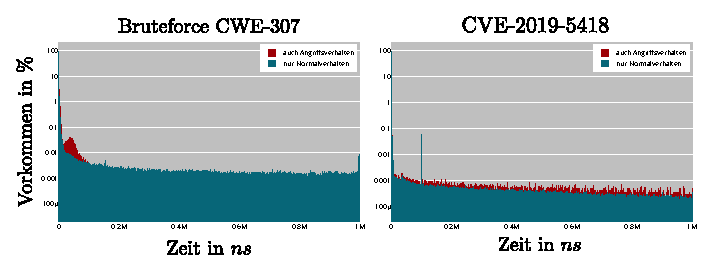
\includegraphics[width=\textwidth]{images/CVE-2012--Test-data-time_delta.eps}
                        \caption[Zeitliche Abstände zwischen System Calls]{Dargestellt ist der zeitliche Abstand zwischen zwei System Calls aus dem selben Thread.
                                 Diese werden in ihrer Häufigkeit in Prozent an allen auftretenden Abstände in dem Plot eingetragen.
                                 Verwendet wurden dafür nur die Testdaten. Links für das Bruteforce Szenario und rechts für das CVE-2019-5418 Szenario.
                                 Blau: Nur Normalverhalten, Rot: Normalverhalten und Angriffsverhalten}
                        \label{fig:time_delta}
                    \end{figure}

                    Die Umsetzung der beschriebenen Idee wird erreicht indem der zeitlichen Abstand $\tau$ zwischen zwei aufeinanderfolgenden System Calls berechnet wird.
                    Dieser wird normalisiert als weiterer Eingabeparameter für den verarbeitenden Algorithmus verwendet.
                    In der Trainingsphase wird zunächst nur der größte Abstand $\tau_{max}$ aus den Trainingsdaten ermittelt.
                    Mithilfe dieses Wertes werden dann in der Testphase alle Werte wie in \autoref{eq:time_norm} beschrieben normalisiert.
                    \begin{equation}\label{eq:time_norm}
                        \tau_{norm} = \frac{\tau}{\tau_{max}}
                    \end{equation}
                    So gilt für die meisten Werte $\tau_{norm}=[0;1]$.
                    Falls $\tau\geq\tau_{max}$ gilt, kann dieser Wert auch größer als $1$ werden.

                    Doch treten mit der Verwendung dieser Information als Extraparameter zwei Probleme auf.
                    Zum einen stellt sich die Frage, ob eine Verbesserung eines Szenarios mit abweichenden Abständen\marginpar{zw. Normal- und Angriffsverhalten} eine Verschlechterung in Szenarien in welchen dies nicht der Fall ist zur Folge hat.
                    Und zum anderen stellt sich die generelle Frage ob diese Information den möglichen Ergebnisraum wesentlich vergrößert worunter die Ergebnisqualität im Gesamten leidet.
                    Denn das Betriebssystem selbst beeinflusst die Timings der System Calls.
                    So können Informationen eingebettet werden welche wenig Aussagekraft über das Normalverhalten eines Prozesses haben.
                    Ob dies das Lernen des Normalverhaltens verbessert oder verschlechtert wird in \autoref{sec:erg_LSTM_extra} untersucht.
                    %\begin{figure}
                        %\centering
                        %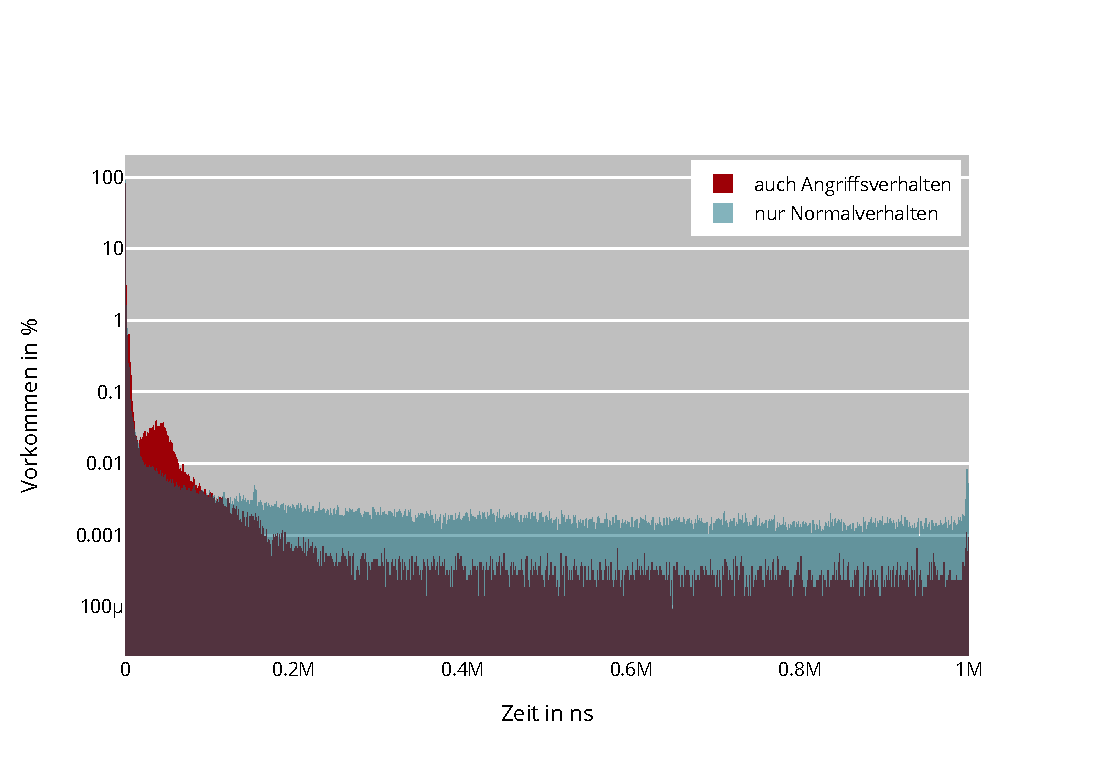
\includegraphics[width=\textwidth]{images/CVE-2012--Test-data-time_delta.pdf}
                        %\caption{Dargestellt ist der zeitliche Abstand zwischen zwei System Calls aus dem selben Thread.
                                 %Diese werden in ihrer Häufigkeit in Prozent an allen auftretenden Abstände in dem Plot eingetragen.
                                 %Verwendet wurden dafür nur die Testdaten des 
                                 %Blau: Nur Normalverhalten}
                        %\label{fig:time_delta_werte}
                    %\end{figure}

                \paragraph{Return Werte}

                    Wie in \autoref{sec:syscall_allg} angemerkt, besteht ein System Call aus zwei \glqq Phasen\grqq.
                    Wobei die zweite Phase den Rückgabewert des Betriebssystemskernel beinhaltet.
                    Bei erfolgreicher Durchführung besteht dieser Rückgabewert bei verschiedenen System Calls aus einem positiven Integerwert.
                    Ist die Durchführung jedoch nicht erfolgreich wird ein Fehler zurückgegeben.
                    Dieser besteht aus einem negativen Integerwert und in manchen Fällen noch einem zusätzlichem Fehlercode.
                    So gibt der Rückgabewert eines \textit{write} System Calls an, wieviele Bytes gelesen wurden.
                    Auch weitere schreibende und lesende System Calls geben die gelesene oder geschriebene Bytes zurück.
                    Für manche System Calls die im Zusammenhang mit Sockets stehen gilt dies ebenfalls.
                    Der Rückgabewert enthält in diesen Beispielen also Informationen über den tatsächlichen Ablauf des spezifischen System Calls.
                    Im Folgenden wird beschrieben wie diese Zusatzinformation der Rückgabewerte kodiert werden kann.
                    Dabei werden nur System Calls betrachtet welche Daten schreiben oder lesen und Daten über Sockets empfangen oder senden. 
                    Zusätzlich wird dies nur für System Calls welche auch im Datensatz vorkommen und einen Byte Rückgabewert haben untersucht.
                    Leider fallen dabei System Calls wie \textit{send} heraus, da der Rückgabewert die Anzahl der gesendeten Charaktere angibt und nicht die Anzahl an geschriebenen Bytes.
                    Es kann also nicht davon ausgegangen werden, dass jegliche schreibende oder lesende Aktion damit abgedeckt ist.
                    In \autoref{tab:syscall_return} werden die den Anforderungen entsprechenden System Calls mit einer Kurzbeschreibung vorgestellt.

                    \begin{table}[ht]
                        \small
                        \centering
                        \begin{tabular}{cp{6cm}p{3cm}}
                            \hline
                            \rowcolor{GruvGray!36}
                            \multicolumn{3}{c}{System Calls}\\
                            \hline
                            Name & Beschreibung & Rückgabewerte\\
                            \hline
                            \hline
                            \rowcolor{GruvGray!16}
                            %open& Öffnet die von \textit{pathname} spezifizierte File. Falls diese nicht existiert kann sie mit dem Zusatz \textit{O_CREAT} automatisch erstellt werden & path, asdklfjs, slddk\\
                            write   & Schreibt angegebene Anzahl an Bytes aus dem Buffer in die Datei, welche über den Filedeskriptor $fd$ definiert wird. & Geschriebene Bytes oder $-1$ bei Fehler\\
                            pwrite  & Schreibt angegebene Anzahl an Bytes aus dem Buffer in die Datei, welche über den Filedeskriptor $fd$ definiert wird. Dabei wird der Datei-Offset nicht geändert.& Geschriebene Bytes oder $-1$ bei Fehler\\
                            \rowcolor{GruvGray!16}
                            writev  & Schreibt \textit{iovcnt} Vektor in die Datei, welche über den Filedeskriptor $fd$ definiert wird.& Geschriebene Bytes oder $-1$ bei Fehler\\

                            read    & Versucht angegebene Anzahl an Bytes von Filedeskriptor \textit{fd} zu lesen und passt den Datei-Offset an.                                              & Gelesene Bytes oder $-1$ bei Fehler\\
                            \rowcolor{GruvGray!16}
                            pread   & Versucht angegebene Anzahl an Bytes von Filedeskriptor \textit{fd} zu lesen und passt den Datei-Offset nicht an.                                        & Gelesene Bytes oder $-1$ bei Fehler\\
                            readv   & Liest spezifizierten \textit{iovcnt} Vektor aus Filedeskriptor \textit{fd} & Gelesene Bytes oder $-1$ Fehler\\

                            \rowcolor{GruvGray!16}

                            sendfile & Kopiert Daten zwischen zwei Filedeskriptoren. Kopiervorgang findet im Kernel statt.& Geschriebene Bytes oder $-1$ bei Fehler\\
                            sendmsg & Übermitteln einer Nachricht an einen anderen Socket. & Gesendete Bytes oder $-1$ bei Fehler\\
                            \rowcolor{GruvGray!16}
                            recv & Empfängt Daten von einem Socket. & Empfangene Bytes oder $-1$ bei Fehler\\
                            \makecell{recvfrom, recvmsg}& Empfängt Daten auf einem Socket welcher nicht zwingend verbindungsorientiert sein muss. & Empfangene Bytes oder $-1$ bei Fehler\\
                            \hline
                        \end{tabular}
                        \caption[Kurzbeschreibung System Calls]{Kurzbeschreibung ausgewählter System Calls.~\cite{SYSCALL_MANPAGE}}
                        \label{tab:syscall_return}
                    \end{table}
                    Diese werden in ihrer Häufigkeit in Prozent an allen auftretenden Rückgabewertgrößen in dem Plot eingetragen. 
                    Für die beschriebenen System Calls werden in \autoref{fig:return_values} die normalisierten Byte Rückgabewerte dargestellt.                
                    Beispielhaft wird dafür das $CVE-2017-7529$ Szenario genutzt.
                    Für die System Calls read, pread und readv sind die Rückgabewertgrößen im Normalverhalten wie im Normalverhalten mit zusätzlichem Angriffsverhalten gleich und zwar ca.\ $615$ Bytes.
                    Bei allen anderen betrachteten Rückgabewerten ist ein Unterschied in den auftretenden Größen bei zusätzlichem Angriffsverhalten zu erkennen.
                    So zum Beispiel bei den write, pwrite, und writev System Calls.
                    Im Normalverhalten werden entweder $100$ oder ca. $250$ Bytes geschrieben, im Angriffsverhalten kommen noch weitere sehr selten auftretende Größen vor.
                    Auch hier gilt analog zu den Zeitabständen für die Normalisierung $\rho_{norm}$ mit einem Rückgabewert $\rho$ und dem Maximalwert aus den Trainingsdaten $\rho_{max}$ aus den Trainingsdaten:
                    \begin{equation}\label{eq:return_norm}
                        \rho_{norm} = \frac{\rho}{\rho_{max}}
                    \end{equation}
                    Neben dem normalisierten Rückgabewert kann aber auch ein Fehlerwert Details über den Ablauf, eines System Calls liefern.
                    Wie in \autoref{tab:syscall_return} beschrieben wird bei diesen System Calls bei nicht erfolgreicher Durchführung eine $-1$ zurückgegeben.
                    Weshalb $\rho_{norm} = -1$ gilt, falls ein System Call aus \autoref{tab:syscall_return} einen Fehlerwert liefert.
                    %TODO noch mehr schreiben?
                    Wie sich die Verwendung der normalisierten Rückgabewerte spezieller System Calls auf die Ergebnisse auswirkt wird in \autoref{sec:erg_LSTM_extra} behandelt.
                    
                    \begin{figure}[ht]
                        \centering
                        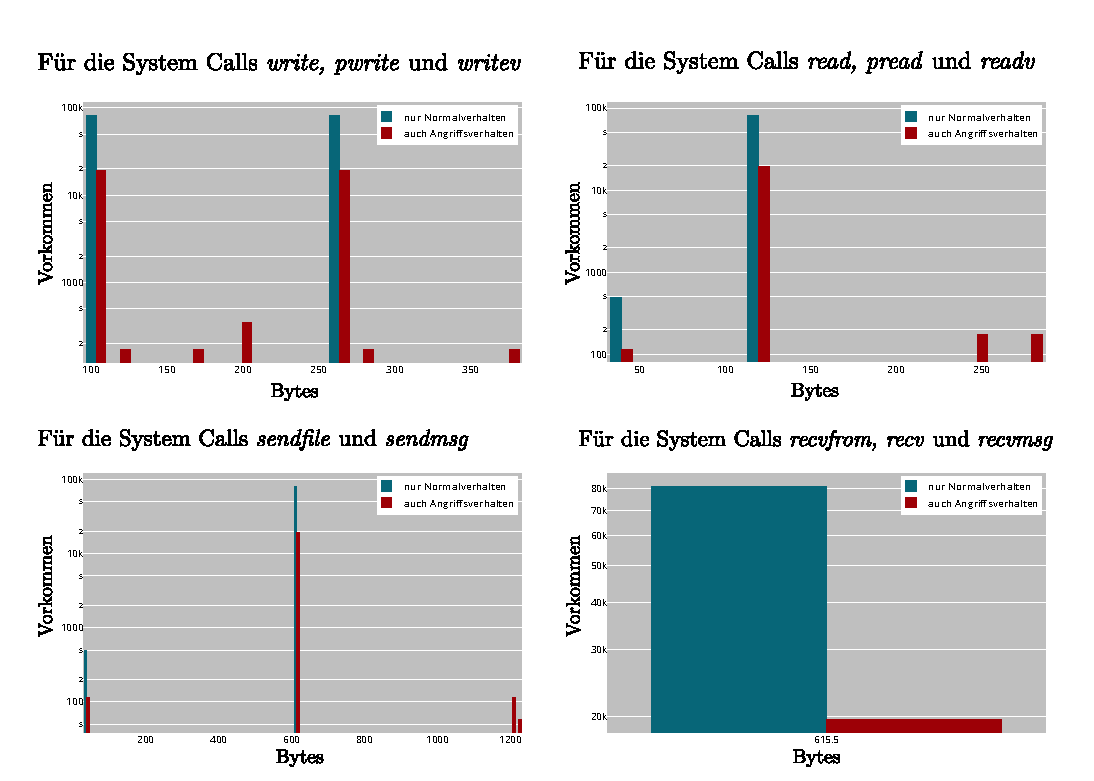
\includegraphics[width=\textwidth]{images/return_2017_plot.pdf}
                        \caption[Histogramm der geschriebenen und gelesenen Bytewerte]{Histogramm der gelesenen/erhaltenen Bytes für die Testdaten des \ac{LID-DS}~\cite{LID-DS} $CVE-2017-7529$ Szenarios.
                        Dargestellt wird dabei immer der Anteil einer Rückgabewertgröße in Byte an allen Rückgabewertgrößen der besagten System Calls.
                        Links oben für die von den System Calls \textit{write, pwrite} und \textit{writev} geschriebenen Bytes.
                        Rechts oben für die von \textit{read, pread} und \textit{readv} gelesenen Bytes.
                        Links unten für die von \textit{sendfile} und \textit{sendmsg} über Sockets gesendete Bytes.
                        Rechts unten für die von \textit{recvfrom, recv} und \textit{recvmsg} über Sockets erhaltenen Bytes.
                        Blau: Nur Normalverhalten, Rot:Normalverhalten und Angriffsverhalten}
                        \label{fig:return_values}
                    \end{figure}

        \subsection{Darstellung eines System Call Streams}\label{sec:streamdarstellung}
            Nachdem die Kodierung eines System Calls und zwei weiterer Parameter neben dem Namen selbst besprochen wurde, soll in diesem Abschnitt die Abarbeitung mehrerer System Calls für den verarbeitenden Algorithmus behandelt werden.
            Dabei werden die Abfolge der System Calls des Datensatzes als ein kontinuierlicher Stream betrachtet.
            Dies ermöglicht den Einsatz der entwickelten Vorgehensweise in der Praxis auch im Live-Betrieb, sofern die Verarbeitung entsprechend schnell stattfindet.
            Für viele Algorithmen wie zum Beispiel auch neuronale Netze ist es sinnvoll und teilweise unausweichlich eine feste Eingangsgröße festzulegen.
            Um dies für einen Stream zu ermöglichen werden in der \ac{NLP} schon seit langer Zeit N-Gramme verwendet~\cite{NGRAMSUEN1979}.
            Auch in der auf System Call basierten Anomalieerkennung kommen N-Gramme zum Einsatz~\cite{STIDE_Alternatives, SYSCALL_GRAPHS, IDSTHREADGRIMMER2021}.
            Ein N-Gramm ist eine zusammenhängende Folge von $n$ Elementen aus einer gegebenen Eingabe.
            Diese werden wie in der linken Grafik in \autoref{fig:ngram_thread} Beispielhaft dargestellt aufgebaut.

            Dabei wird ein Buffer der Länge $n$ erzeugt, welcher das erste n-gram liefert sofern sich $n$ Elemente in dem Buffer befinden.
            Kommt ein neues Element in den Buffer fällt das älteste heraus.

            Zu beachten ist dabei, dass die Abfolge der System Calls mehrere logische Abfolgen zusammenführt.
            Denn moderne Computer Systeme verarbeiten mehrere Threads parallel.~\cite{SYSCALL_SILBERSCHATZ}
            Die System Calls aller Threads werden dann je nach dem wie sie vom Betriebssystemskernel verarbeitet werden an die Sequenz angefügt.
            
            \paragraph{Thread Awareness}
                Grimmer et al.~\cite{IDSTHREADGRIMMER2021} beschreiben in ihrer Arbeit wie sie die Thread Information der System Calls verwenden um die verwundenen Sequenzen zu entwirren.
                Dabei werden für jeden Thread ein eigener Buffer erzeugt. 
                Die Ausgabe dieser Buffer wird in der rechten Grafik in \autoref{fig:ngram_thread} veranschaulicht. 
            Also nur System Calls aus demselben Thread bilden ein n-gram, weshalb sie von \textit{Thread aware} N-Grammen\marginpar{zu dt.\ Thread bewusst} sprechen.
                Grimmer et al.\ konnten zeigen, dass dies speziell auch für diesen Datensatz eine Verbesserung der Ergebnisse erzielt.
                Darüber hinaus zeigen sie, dass bei der Verwendung von \textit{Thread aware} N-Grammen im Vergleich zu n-grammen ohne Berücksichtigung von Threads in keinem Szenario eine Verschlechterung der Ergebnisse auftritt.

                \begin{figure}
                    %thread ngram image
                    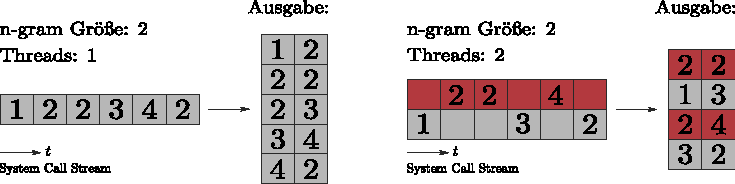
\includegraphics[width=\textwidth]{images/ngram.pdf}
                    \caption[Erstellung N-Gramme]{Erstellung der N-Gramme mit $n=2$ aus einem Datenstream von System Calls.
                        Links ohne und rechts mit der Beachtung der Threadinformation.
                        Die dabei entstehenden N-Gramme dienen als Eingabe für den bewertenden Algorithmus.
                        Die Reihenfolge der entstehenden N-Gramme als Eingaben ist dabei von oben nach unten.
                    }\label{fig:ngram_thread}
                \end{figure}

            \paragraph{Thread Change Flag}
                Sie verwenden in der Auswertung aber ausschließlich Algorithmen welche kontextfrei arbeiten.
                Dies bedeutet, dass zuvor gesehene N-Gramme keinen Einfluss auf das aktuelle haben.
                Wie in~\autoref{sec:LSTM} beschrieben wird, ist das bei \ac{LSTM} Netzwerken nicht der Fall.
                Es gilt also den benötigten Kontext in die von Grimmer et al.\ beschriebene Methodik zu integrieren.

                Eine Möglichkeit bestünde darin die ThreadID zu kodieren und die Information aus welchem Thread das n-gram stammt mitzugeben.
                Doch das Kodieren der tatsächlichen Thread ID ist sehr unpraktisch, da Thread IDs wiederverwendet werden können.
                Stattdessen wird in dieser Arbeit ein n-gram mit der Informatione über einen Kontextwechsel angereichert. 
                Dieser Kontextwechsel soll dann über die \ac{TCF} an das \ac{LSTM} übergeben werden.
                Initial wird, weil kein Kontextwechsel stattfindet, für die \ac{TCF} eine $0$ angegeben.
                Kommt das aktuelle n-gram aus demselben Thread wie das n-gram zuvor, ist die \ac{TCF} ebenfalls $0$.
                Ist das aktuelle n-gram allerdings aus einem anderen Thread wird ein Kontextwechsel durch das Setzen der \ac{TCF} auf $1$ angezeigt.
                Visualisiert wird dies in \autoref{fig:ngram_tcf}.

                \begin{figure}[ht]
                    %thread ngram image
                    \centering
                    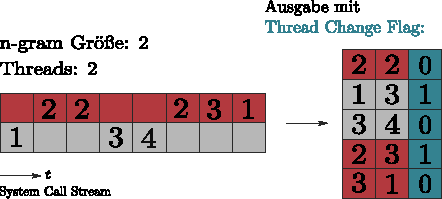
\includegraphics[width=0.6\textwidth]{images/tcf.pdf}
                    \caption[Erstellung Thread Aware N-Gramme]{Analog zu \autoref{fig:ngram_thread} werden N-Gramme erzeugt.
                             Diese werden nun mit der \ac{TCF} angereichert.
                             Initial ist die \ac{TCF} $0$.
                             Ist das zuvor ausgegeben n-gram aus demselben Thread, ist die \ac{TCF} ebenfalls $0$.
                             Findet ein Wechsel des Threads statt, wird dieser Kontextwechsel durch das Setzen der \ac{TCF} auf $1$ signalisiert.}\label{fig:ngram_tcf}
                \end{figure}

                Die Vorstellung dabei ist, dass eine \ac{TCF}$= 1$ dem \ac{LSTM} die Information gibt, dass der zuvor gesehene N-Gramme nur eine untergeordnete Rolle für den Kontext spielen, da diese aus einem anderen Thread stammen.
                Falls dies der Fall ist, kann ein häufiger Kontextwechsel dafür sorgen, dass der Vorteil der \ac{LSTM}s abgeschwächt wird, da immer dafür gesorgt wird, dass potentiell wenige Informationen im Kontext enthalten sind.
                In \autoref{tab:tcf} wird dargestellt wie oft so ein Kontextwechsel stattfindet.
                Dabei ist zu erkennen, dass in den Szenarien aus dem \ac{LID-DS} bei einer Länge von $n=6$ nur bis zu $13.8\%$ der N-Gramme eine $\ac{TCF}=1$ haben.
                Die zuvor geschilderte Gefahr scheint also für die gegebenen Szenarien keine Rolle zu spielen, ist aber für andere Einsatzbereiche mit nicht kontextfreien verarbeitenden Algorithmen zu beachten.

                \begin{table}[ht]
                    \small
                    \centering
                    \begin{tabular}{lrrr}
                        \hline
                        \rowcolor{GruvGray!36}
                        \multicolumn{4}{c}{Thread Change Flag}\\
                        \toprule
                        Szenario & \#\ac{TCF}$=1$ & \#\ac{TCF}$=0$ & \makecell{Anteil \ac{TCF}$=1$ \\an allen N-Grammen \\ in \%}\\
                        \midrule
                        \rowcolor{GruvGray!16}
                        $Bruteforce\_CWE\_307$ & $2,534,165$ & $20,383,314$ & $11.1$ \\
                        $CVE-2012-2122$ & $1,206,151$ & $10,365,309$ & $10.4$ \\
                        \rowcolor{GruvGray!16}
                        $CVE-2014-0160$ & $1,120,786$ & $7,026,864$ & $13.8$ \\
                        $CVE-2017-7529$ & $1,130,717$ & $10,721,010$ & $9.5$ \\
                        \rowcolor{GruvGray!16}
                        $CVE-2018-3760$ & $1,453,876$ & $38,255,576$ & $3.7$ \\
                        $CVE-2019-5418$ & $3,131,792$ & $74,159,462$ & $4.1$ \\
                        \rowcolor{GruvGray!16}
                        $PHP\_CWE-434$ & $10,891,051$ & $112,549,739$ & $8.8$ \\
                        $EPS\_CEW-434$ & $12,657,844$ & $374,439,042$ & $3.3$ \\
                        \rowcolor{GruvGray!16}
                        $ZipSlip$ & $80,126,899$ & $444,510,136$ & $15.3$ \\
                        \hline
                    \end{tabular}
                    \caption[Häufigkeit eines Kontextwechsels]{Vorkommen von eines Kontextwechsels angezeigt durch die \ac{TCF}.
                    Bei einer n-gram Länge von $6$.}
                    \label{tab:tcf}
                \end{table}

    \section{Aufbau des \acp{LSTM}}\label{sec:aufbau_lstm}
        \begin{figure}[ht]
            \centering
            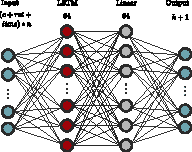
\includegraphics[width=0.7\textwidth]{images/lstm.pdf}
            \caption[Aufbau des \ac{LSTM}]{Aufbau des \ac{LSTM} mit $64$ Neuronen für die \ac{LSTM}- und Linear-Layer.
                Die Input Layer besitzt $(e + ret + time) * n$ Neuronen, mit $e$ für die Größe des \ac{W2V}-Embeddings,
                $ret=1$ falls Rückgabewerte verwendet werden und $time=1$ falls die Zeitabstände verwendet werden.
                Ansonsten sind $ret=0$ und $time=0$.
                Und die Output Layer hat $k+1$ Ausgangsneuronen, dabei ist $k$ die Anzahl an System Calls aus dem Trainingsdatensatz.
                Eins wird addiert für unbekannte System Calls.}
                \label{fig:lstm}
        \end{figure}

        Die Architektur wird ebenfalls in \autoref{fig:lstm} dargestellt und besteht aus der Eingabe-Layer, der \ac{LSTM}-Layer, einer \textit{fully-connected} Linear-Layer und der Output-Layer.
        Wie dargestellt, wird für die Initialisierung der Implementierung des \acp{LSTM} die Anzahl an Input und Output Neuronen benötigt.
        Für die Eingangsgröße gilt:
        \begin{equation}
            input\_dim = (e + ret + time) \cdot n + \ac{TCF}
        \end{equation}
        Mit $e$ für die gewählte Größe des \ac{W2V}-Embeddings.
        Falls der zuvor beschriebene Zusatzparameter für die Rückgabewerte verwendet wird gilt $ret=1$ ansonsten $ret=0$.
        Gleiches gilt für den Extraparameter welcher die Zeitabstände kodiert und Kontextwechsel angebende \ac{TCF}.
        Für die Ausgangsgröße gilt:
        \begin{equation}
            output\_dim = k + 1
        \end{equation}
        Dabei ist $k$ die Anzahl an System Calls aus dem Trainingsdatensatz, eins wird addiert für unbekannte System Calls, also System Calls in den Testdaten welche noch nicht im Trainingsdatensatz auftraten.
        Nötig ist diese Variabilität, da für die Initialisierung des \acp{LSTM} die Anzahl der verschiedenen System Calls im Trainingsdatensatz für die Ausgangsgröße, sowie die Eingangsgröße des System Calls eine Rolle entscheidende Rolle spielt.

        Festgelegt werden hingegen Größen für die \textit{Hidden Layer} Dimension, \textit{Batch Size}, den \textit{Optimizer}, die \textit{Loss}-Funktion und die Lernrate.
        Die Dimension der \ac{LSTM}-Layer wird auf $64$ gesetzt, die \textit{Batch Size} auf $1024$.
        Es wird der für \acp{LSTM} gängige \textit{Adam Optimizer} gewählt.
        Da es sich um eine Klassifikation mit $k+1$ Klassen handelt, wird die \textit{Cross-Entropy} Loss-Funktion des PyTorch Frameworks genutzt.
        Die Lernrate wird auf $0.001$ festgelegt.
        Details zu der Parameterwahl wird in \autoref{sec:parameterwahl} erläutert.

        Entgegen der typischen Implementierungen von \acp{LSTM} wird der \textit{Hidden State} nach einem Batch gespeichert und dem nächsten Batch  übergeben. 
        Der Hauptgrund dafür ist die Länge der System Call Streams.
        Diese können länger als ein Batch sein, werden die Hidden States nicht übergeben, geht die Kontextinformation zwischen den Batches verloren.
        Diese Idee ist allerdings ausgelegt für einen kontinuierlichen Stream an System Calls, der Datensatz besteht aber aus vielen Dateien.
        Deswegen wird der \textit{Hidden State} zum Ende einer Aufnahme zurückgesetzt.

        Ausgaben des \acp{LSTM} sind durch die Verwendung der PyTorch CrossEntropy Loss-Funktion sogenannte \textit{Logits}.
        Auf diese kann mithilfe der \textit{Softmax}-Funktion eine Liste an Wahrscheinlichkeiten für jeden System Call sowie den Platzhalter erstellt werden.

    \section{Algorithmus}\label{sec:Algorithmus}
        Im vorigen Kapitel wurden alle verwendeten Vorverarbeitungsschritte vorgestellt.
        In den kommenden Abschnitten werden diese Schritte zu einem Ablauf zusammengeführt.
        Zunächst soll in \autoref{sec:Allgemein} ein allgemeiner Überblick gegeben werden.
        Anschließend wird in \autoref{sec:Training} behandelt was das \ac{LSTM} Netzwerk lernt.
        Schließlich erklären \autoref{sec:Anomalieerkennung} und \autoref{sec:Schwellung}, wie aus dem Gelernten die Klassifizierung in normales oder Angriffsverhalten erfolgt.

        \subsection{Allgemein}\label{sec:Allgemein}
            Wie bereits in \autoref{sec:related_nlp} beschrieben, werden verschiedene Verfahren der \ac{NLP} auch in der anomaliebasierten \ac{HIDS} eingesetzt.
            Neben den bereits beschriebenen \ac{W2V} Verfahren kommen auch die in der \ac{NLP} verbreiteten \ac{LSTM} Netzwerke zum Einsatz.
            Mit dem \ac{LSTM} soll in der Trainingsphase ein Sprachmodell der System Calls erstellt werden.
            Dieses Sprachmodell soll mit einer gegebenen Sequenz $s = (sc_{x_1},\dots,sc_{x_n})$ den folgenden System Call $sc_{x_{n+1}}$ vorherzusagen. 
            Dabei bestehen die Trainingsdaten nur aus Normalverhalten, enthalten also keine Angriffe.
            Anhand dieses gelernten Modells soll dann in der Testphase eine Vorhersage über den nächsten System Call gemacht werden.
            Diese Vorhersage besteht aus den Wahrscheinlichkeiten für alle aus dem Training gesehenen System Calls, plus einem Platzhalter für noch unbekannte System Calls.
            Die Wahrscheinlichkeit des tatsächlich auftretenden System Calls von eins abgezogen stellt dann den Anomaliescore dar.
            Ob dieser Anomaliescore zu einem Alarm führt oder nicht, hängt von einem zuvor bestimmten Schwellwert ab.
            Dieser wird bestimmt, indem nach dem Training die Anomaliescores für einen Ausschnitt des Datensatzes bestimmt werden.
            In diesem Ausschnitt, auch Validierungsdaten genannt, darf wie in den Trainingsdaten kein Angriffsverhalten enthalten sein.
            Eine Garantie die in der echten Welt nie komplett gegeben werden kann.
            In den Validierungsdaten soll folglich kein Alarm ausgelöst werden, weshalb der höchste Anomaliescore der Validierungsdaten als Schwellwert der Anomalieerkennung verwendet wird.
            Dies ist eine Annäherung an einen optimalen Schwellwert.

            Die System Calls werden wie zuvor beschrieben durch das \ac{W2V} Verfahren in einen Vektor umgewandelt und durch die zwei zuvor beschriebenen Verfahren, die Normalisierung der Zeitabstände und der Rückgabewerte bestimmter System Calls, angereichert.
            Der Stream der System Calls wird dann mit Betrachtung der Threads in N-Gramme zusammengetragen.
            Zusätzlich wird zu jedem n-gram die Information über einen Kontextwechsel durch die \ac{TCF} angegeben.
            % Im Folgenden wird der Trainingsablauf detaillierter bestimmt.

        \subsection{Training}\label{sec:Training}
            \begin{figure}
                \centering
                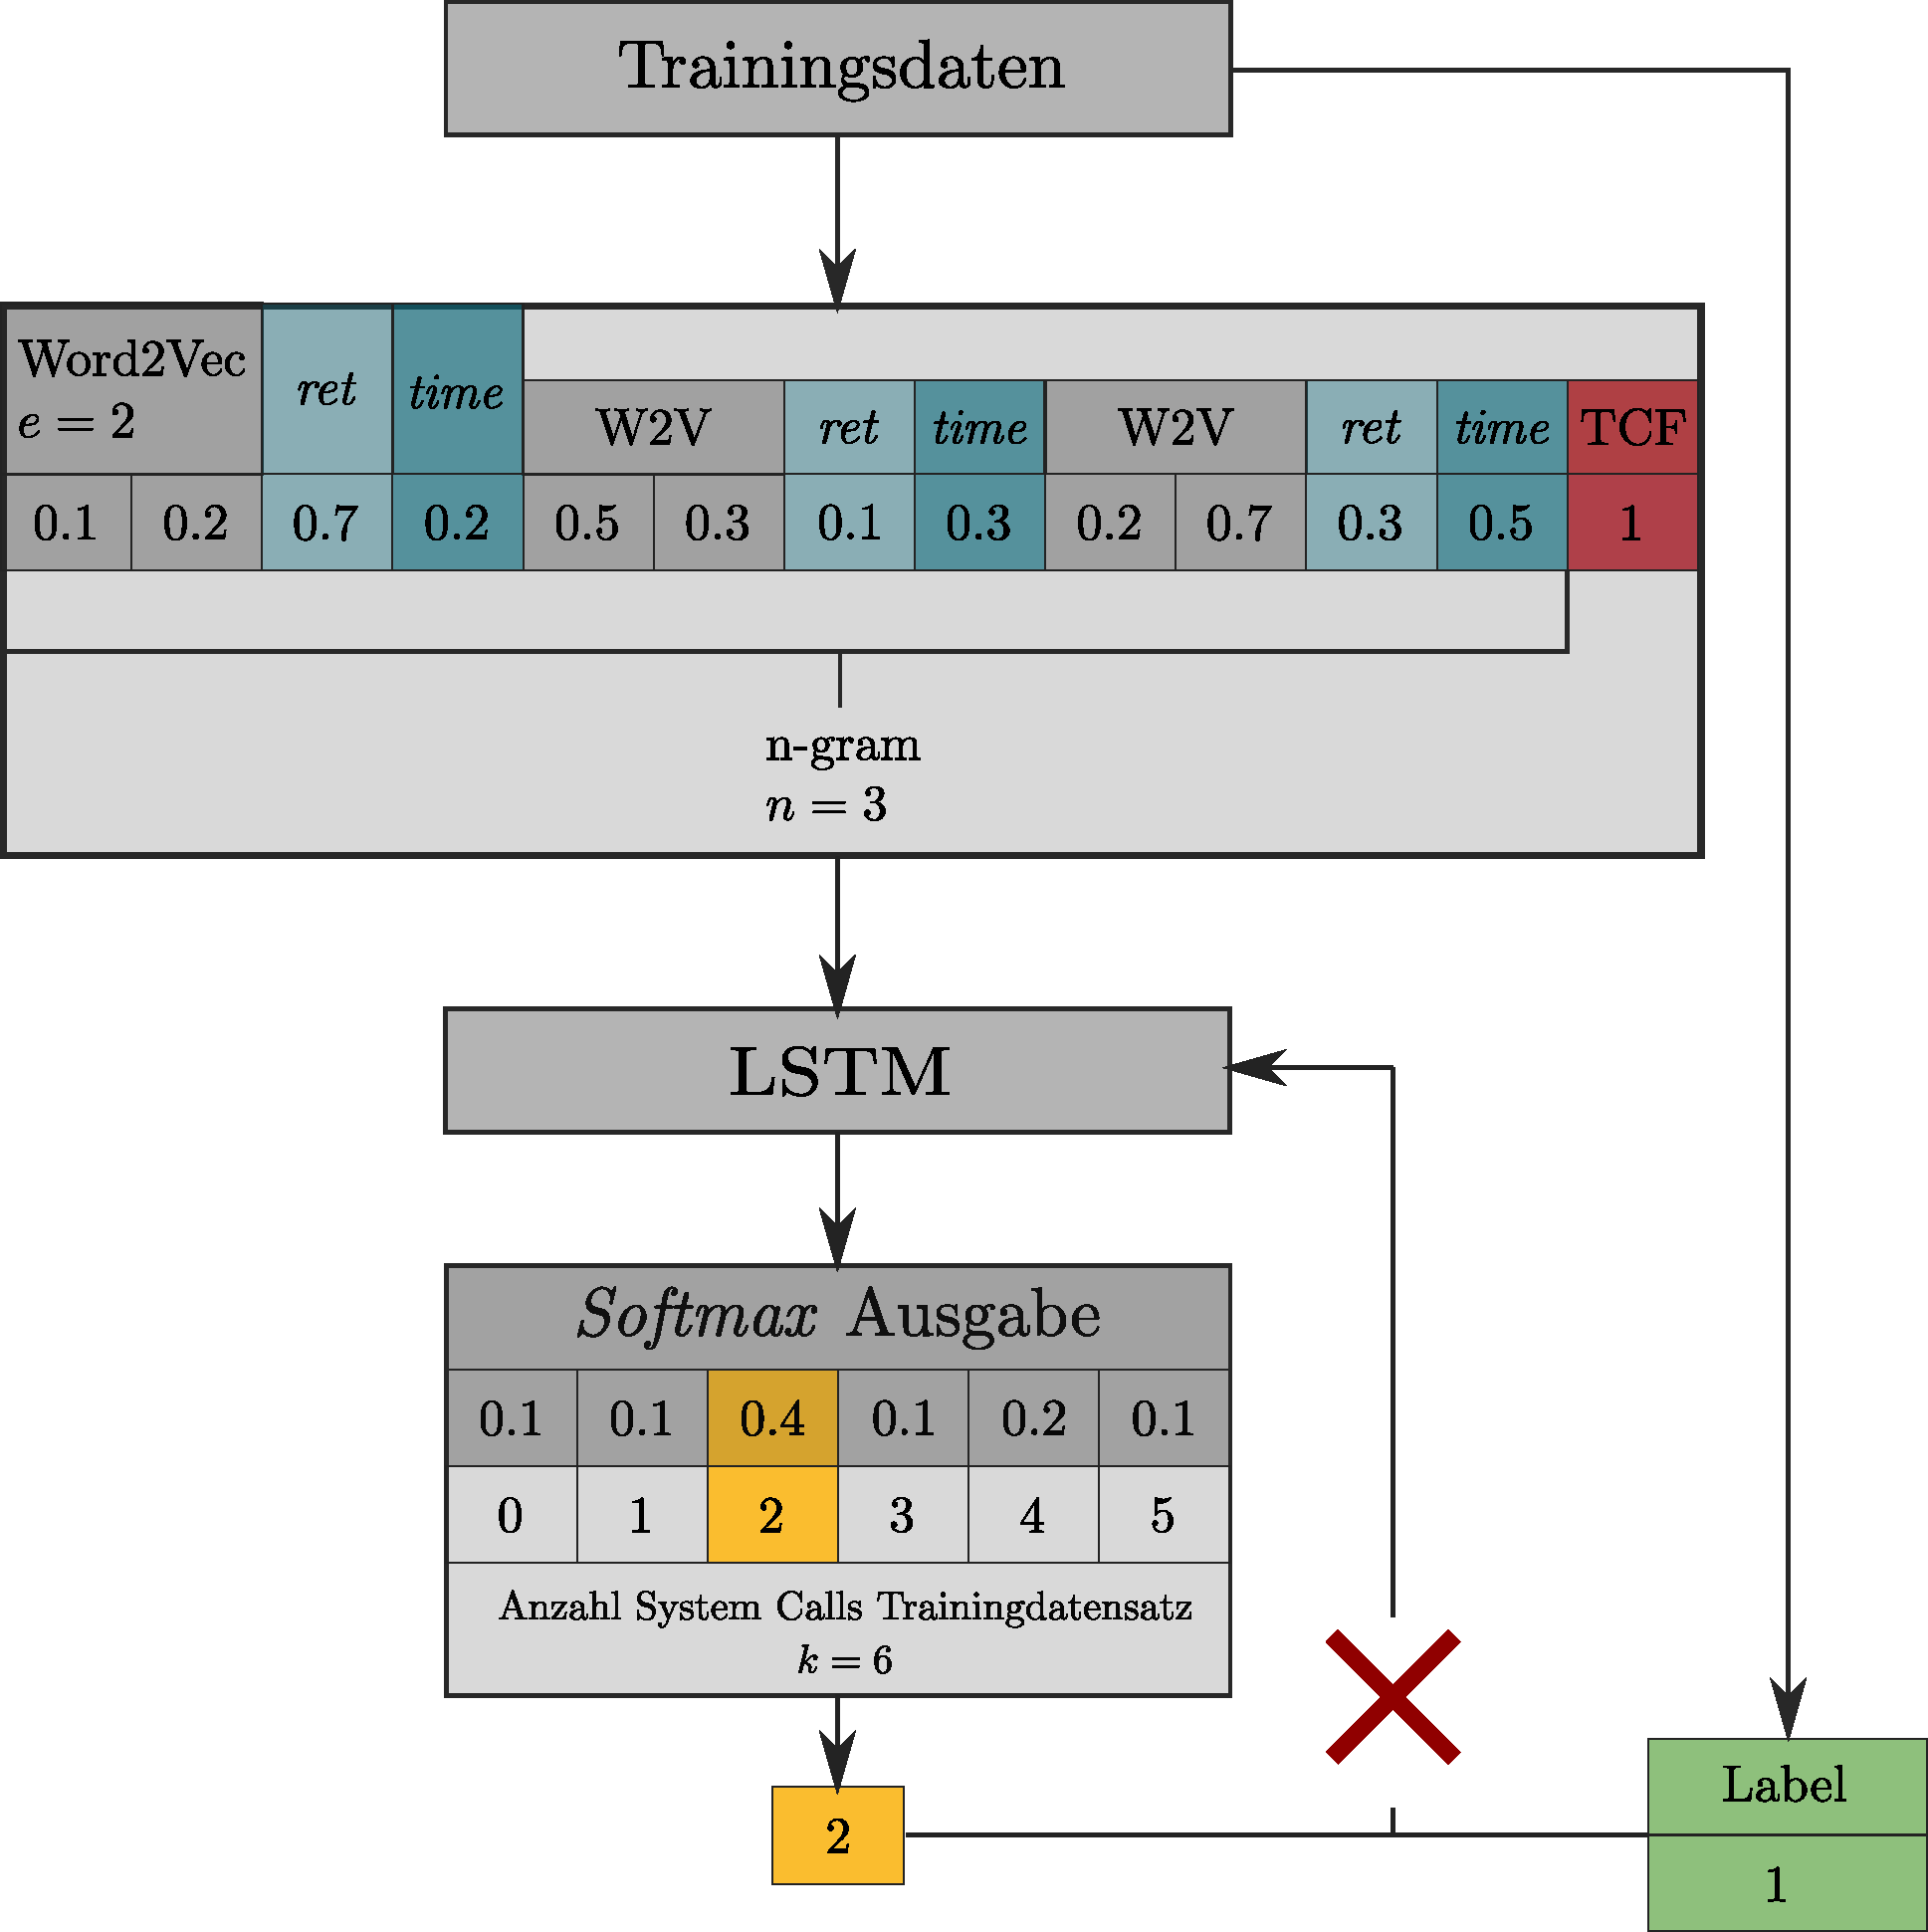
\includegraphics[width=0.75\textwidth]{images/Process_overview.pdf}
                \caption[Algorithmus - Ablauf Trainingsphase]{Ablauf der Trainingsphase mit Beispieldaten.
                        Aus Trainingsdaten wird ein n-gram aus \ac{W2V}, Rückgabewert (\textit{ret}) und Zeitabstand (\textit{time}) erstellt.
                        Diese beiden Extraparameter sind bläulich hervorgehoben.
                        Zusätzlich wird die \ac{TCF} an das n-gram gefügt.
                        Der Index des höchsten Wertes (gelb) aus der Ausgabe des \ac{LSTM} wird mit dem eigentlichen Label (grün) verglichen.
                        Aufgrund dieser Information werden die Gewichte im \ac{LSTM} angepasst}\label{fig:training}
            \end{figure}
            % Für das Training des \ac{LSTM} Netzwerkes werden nur Normaldaten aus dem Trainingsdatensatz verwendet.
            Pro Szenario werden $200$ Aufnahmen ohne Angriffsverhalten, der insgesamt ca.\ $1100$ Aufnahmen, für das Training ausgewählt.
            Die Grundidee besteht wie zuvor beschrieben darin, mit einer gegebenen Sequenz $s = (sc_{x_1},\dots,sc_{x_n})$ den folgenden System Call $sc_{x_{n+1}}$ vorherzusagen. 
            Da der nächste System Call aus dem Datensatz stets bekannt ist, kann als Feedback für das Netzwerk die Information genommen werden, ob $sc_{x_{n+1}}$ korrekt vorhergesagt wurde, also dem Label entspricht.
            Das \ac{LSTM} gibt wie in \autoref{fig:training} dargestellt diese Information an das \ac{LSTM} zurück.

            Seien die System Calls aus den Trainingsdaten aus der Menge $SC = \{sc_1,sc_2,\dots,sc_k\}$.
            Womit $k$ die Anzahl der in den Trainingsdaten vorkommenden System Call Namen angibt.
            Die Trainingsdaten werden durchlaufen und N-Gramme $ngram_i$ erstellt.
            Der auf das $ngram_i$ folgenden System Call dient als Label $l_i$.
            Nach dieser Idee ist das erste n-gram $ngram_0$ mit Label $l_0$.
            Dabei werden die System Call Namen für die Label durch Integerwerte ersetzt. 
            Das \ac{LSTM} Netzwerk bekommt $ngram_0$ und gibt einen Vektor der Länge $k+1$ zurück.
            Dieser Vektor gibt für jeden der $k$ möglichen System Calls aus den Trainingsdaten eine Auftrittswahrscheinlichkeit an.
            Zusätzlich wird $1$ addiert, da in den Testdaten unbekannte System Calls auftreten können.
            Diese bekommen den \ac{W2V}-Vektor $(0)^e$, wobei $e$ die Länge des \ac{W2V}-Vektoren ist oder für das Label einen Integerwert von $0$. 
            Die Ausgabe des \acp{LSTM} sind \textit{PyTorch Logits}, diese werden mithilfe der \textit{Softmax}-Funktion in die gewünschten Wahrscheinlichkeiten umgewandelt.
            Der Index der Liste der so berechneten Wahrscheinlichkeiten wird mit dem aus den Trainingsdaten gezogenen Label verglichen.
            Dieser Vergleich dient dann als Feedback für das \ac{LSTM}.
            Mit den gegebenen Trainingsdaten kann nun das \ac{LSTM} mittels des \textit{back-propagation through time}  trainiert werden.

        \subsection{Anomalieerkennung}\label{sec:Anomalieerkennung}
            \begin{figure}[ht]
                \centering
                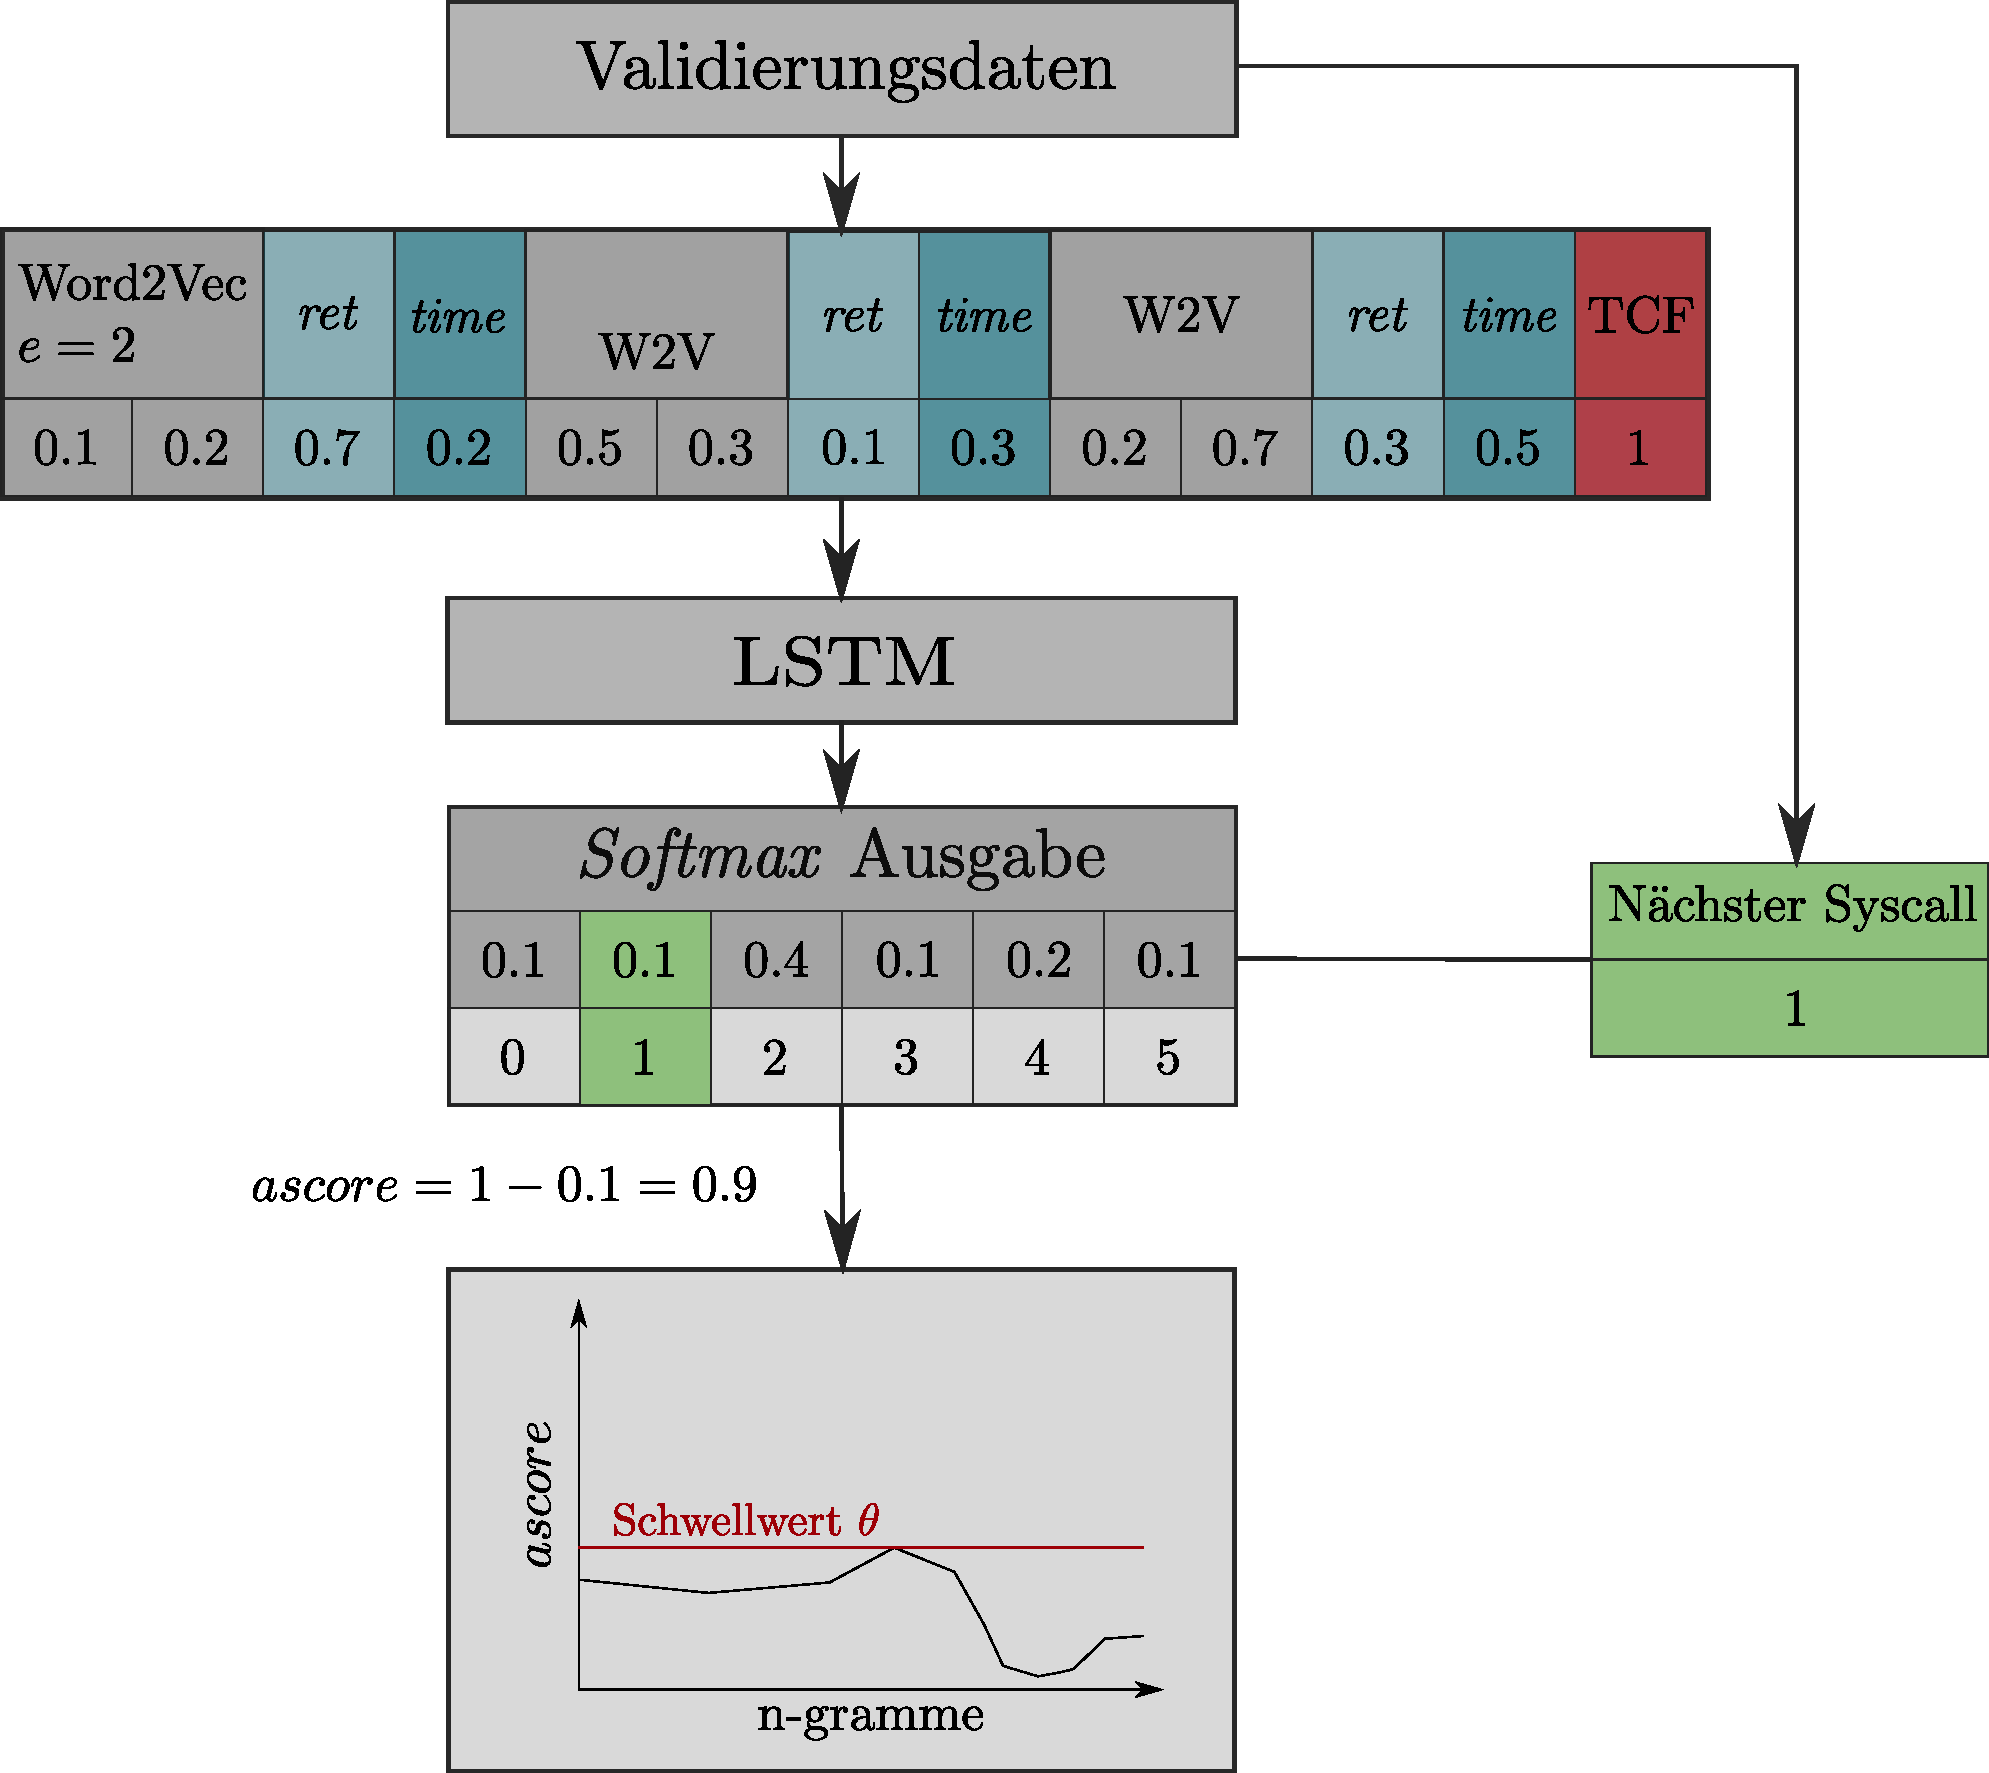
\includegraphics[width=0.8\textwidth]{images/Validation_overview.pdf}
                \caption[Algorithmus - Ablauf Validierungsphase]{Ähnlich zu \autoref{fig:training} wird hier der Validierungsablauf beschrieben.
                         Dabei wird wie zuvor ein Datenauszug dargestellt sowie die Auftrittswahrscheinlichkeiten für den folgenden System Call.
                         In der Test-, wie in der Validierungsphase dient die Wahrscheinlichkeit des Integerwerts des tatsächlich als nächstes auftretende System Call als Berechnungsgrundlage für den Anomaliescore.
                        Wie unten in der Abbildung dargestellt, wird das Maximum der $ascore$s der gesamten Validierungsdaten als Schwellwert festgelegt.}
                \label{fig:validierung}
            \end{figure}
            Es kann also bei Auftreten des System Calls $sc_i$ überprüft werden mit welcher Wahrscheinlichkeit $p_i$ dieser vorhergesagt wurde.
            Der eigentliche Anomalie-Score $ascore$ für $sc_i$ wird dann folgenderweise berechnet:
            \begin{equation}
                ascore = 1 - p_i
            \end{equation}
            Übertrifft dieser Wert einen zuvor bestimmten Schwellwert $\theta$, so wird $sc_i$ als Anomalie und damit als Angriff gewertet.

            \paragraph{Schwellwertbestimmung}\label{sec:Schwellung}
                Für die Berechnung des Schwellwertes $\theta$ wird für alle System Calls der Validierungsdaten $ascore$ berechnet.
                Die Validierungsdaten bestehen aus $50$ Aufnahmen und enthalten ebenfalls wie die Trainingsdaten nur das Normalverhalten.
                Da in den Validierungsdaten kein Angriffsverhalten integriert ist, darf keiner der $ascore$s einen Alarm auslösen.
                Weshalb der höchste Wert der $ascore$s den Validierungs als Schwellwert $\theta$ genutzt wird.
                Der Ablauf der Schwellwertfindung wird zusätzlich in \autoref{fig:validierung} dargestellt.
                Dabei ist ähnlich zu \autoref{fig:training} dargestellt wie ein System Call n-gram kodiert wird und als Eingabe in das \ac{LSTM} dient.
                Zusätzlich wird die Berechnung des $ascores$ dargestellt, indem das Label als Index für die Softmax  Ausgabe des \acp{LSTM} dient.
                Das Maximum der $ascores$ wird wie beschrieben dann als Schwellwert $\theta$ genutzt.

        \subsection{Parameterwahl}\label{sec:parameterwahl}
            Das Aufsetzen des beschriebenen Algorithmus bedarf der Festlegung einiger Parameter.
            Dazu gehören allgemeine Parameter für neuronale Netze, aber auch spezifischere Parameter wie die Länge der N-Gramme.
            Da nicht alle Parameter experimentell untersucht werden können werden sie im Folgenden in festgelegte und zu ermittelnde Parameter unterteilt.
            \paragraph{Festgelegte Parameter}
                Entscheidende Parameter der \acp{LSTM} sind die Anzahl der Neuronen pro Layer sowie die Anzahl der \ac{LSTM}-Layer in dem Netzwerk.
                Da sich bei ersten Tests schnell die Problematik aufgetan hat, dass die Berechnungen sehr großer Szenarien zu nicht tragbaren Laufzeiten geführt hat, muss dies bei der Findung vieler Parameter bedacht werden.
                Deshalb wird in dieser Arbeit nur eine \ac{LSTM}-Layer verwendet, auch wenn in manchen Anwendungen der \ac{NLP} mehrere Layer zu einer verbesserten \textit{Accuracy} führen.\cite{LSTMHYPERAUFA2020}
                Die Anzahl der Neuronen dieser Layer wird wie bereits in \autoref{sec:aufbau_lstm} beschrieben auf $64$ festgelegt.
                Die Lernrate wurde anhand der Ergebnisse mehreren Tests auf wenigen Szenarien auf $0.001$ festgelegt.
                Außerdem wird der für \acp{LSTM} häufig eingesetzte Adam-Optimizer verwendet.
                Diese Einstellungen wurden auch in der Arbeit von Dymshits et al.~\cite{LSTMDYMSHITS2017} eingesetzt.
                Als Loss Funktion wird für das $k+1$ Klassen Klassifizierungsproblem die \textit{Cross-Entropy} gewählt.
                Wie auch in \autoref{fig:learning_rate} erkennbar ist stagniert der Fehler bei verschiedenen Szenarien nach nur wenigen Epochen, weshalb für die Epochenanzahl ein Maximum von $20$ festgelegt wird.
                Der Einfluss der Batch size auf die Ergebnisqualität wird unter anderem in~\cite{LSTMBENCHBREUEL2015} als gering eingestuft und wird auf $1024$ festgelegt.
                 
                
                \begin{figure}
                    \centering
                    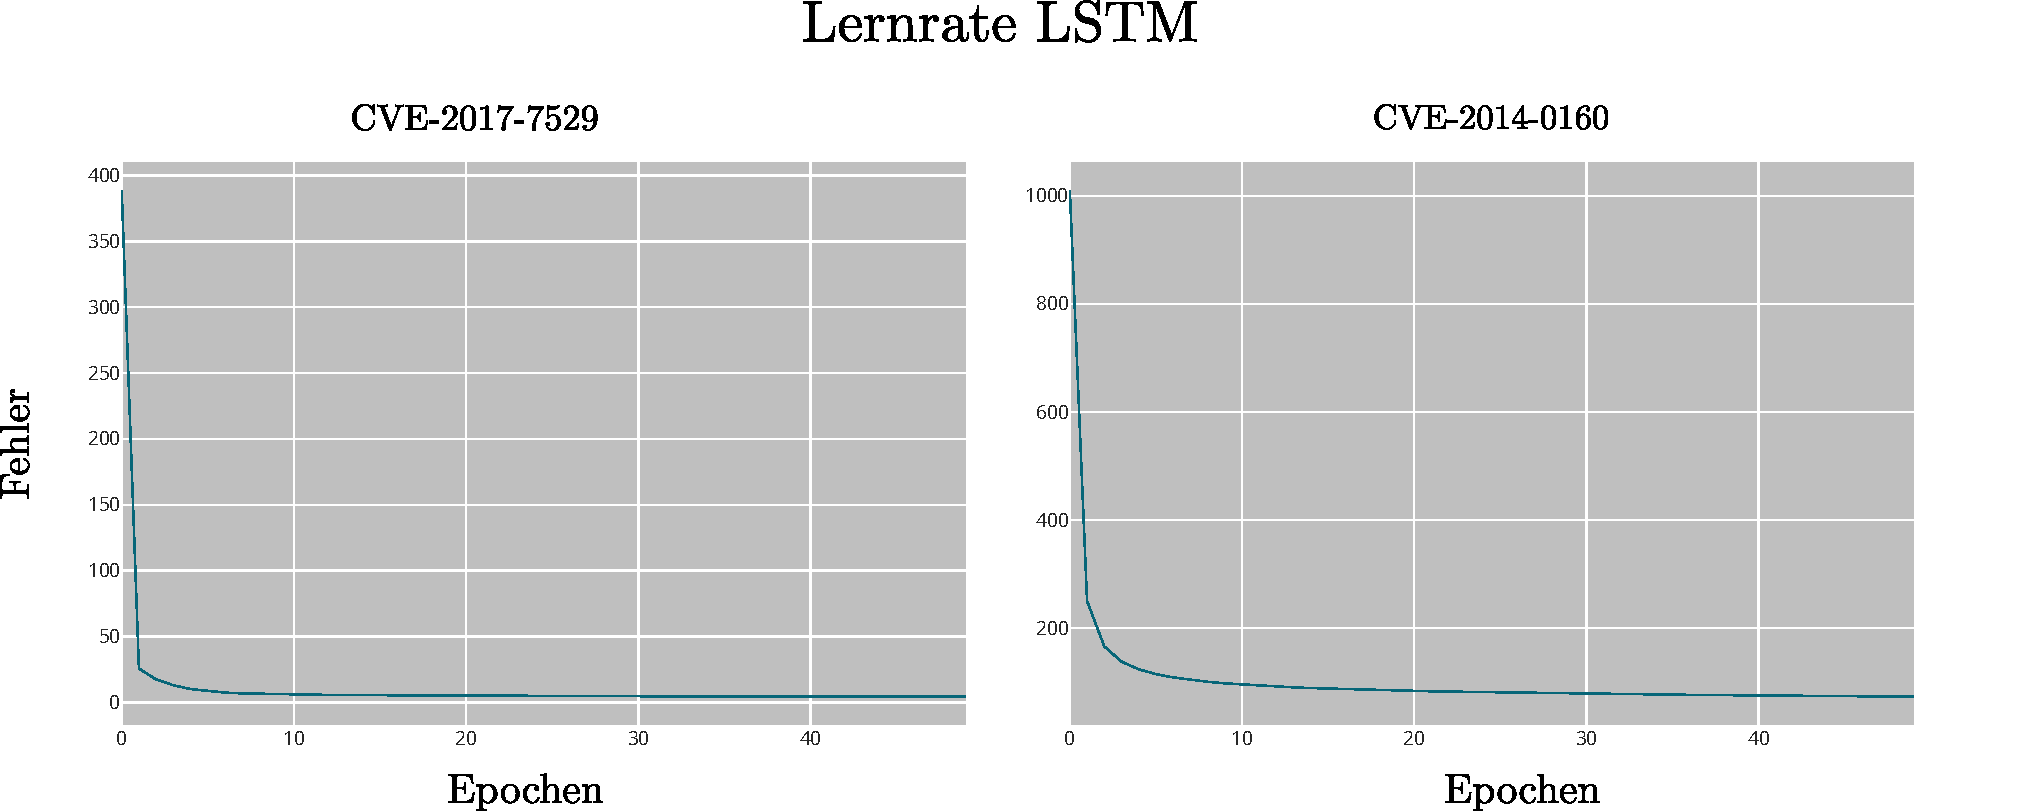
\includegraphics[width=\textwidth]{images/learning_rate.pdf}
                    \caption[Parameterwahl - Fehler während des Trainings]{Darstellung des Fehlers während des Trainingsvorgangs für zwei Szenarien.
                             Zum einen ist ein Lernfortschritt zu erkennen und zum anderen tritt dieser bereits nach wenigen Epochen ein.}\label{fig:learning_rate}
                \end{figure}

                Da das Berechnen des \ac{W2V} im Vergleich zum Training und Testen des \acp{LSTM} nur einen geringen Zeitaufwand benötigt wird eine Epochenanzahl von $500$ festgelegt. 
                Es werden aufgrund der Ergebnissen von Grimmer et al.~\cite{IDSTHREADGRIMMER2021} nach verschiedenen Tests mit alten Konfigurationen nur N-Gramme mit Betrachtung der Thread Information aufgebaut.

            \paragraph{Zu ermittelnde Parameter}
            Ziel ist es eine Konfiguration der Parameter zu finden, mit der alle Szenarien aus dem \ac{LID-DS} mit hoher \ac{DR} und niedriger \ac{FP}-Rate ausgewertet werden können.
            Dafür gilt es speziell verschiedene \textbf{n-gram} Größen in Kombination mit verschiedenen Größen für das \textbf{\ac{W2V}-Embedding} zu finden.
            Für die n-gram Größen wurden $[2,6,10]$ und für das \ac{W2V}-Embedding $[4,6,8,10]$ zur Auswahl gestellt.
            Zusätzlich soll untersucht werden ob sich durch die Hinzunahme weiterer System Call Parametern neue erfolgreiche Konfigurationen ergeben.
            Speziell wird getestet ob sich \textbf{\ac{TCF}}, \textbf{Rückgabewerte}, \textbf{zeitliche Abstände} oder jegliche \textbf{Kombinationen} dieser positiv auf die Ergebnisse auswirken.
                
\iffalse
    \section{Strukturierung der Experimente}\label{sec:StrukExp}
        Um aussagekräftige Experimente zu entwickeln müssen zuerst 
        überlegungen zur praktischen umsetzung gemacht werden
        dabei wird in ersten Tests klar, dass zeit hierbei eine große rolle spielen wird

        erste Tests also ausgelegt um Faktoren zu ermitteln, welche die auswertungen stark verlangsamen
        und diese ausschließen.

        \subsection{Faktor Zeit}
            zeit/dr als groesse und farbe von scatter plot
            batch size test und train x/y achse

            eingrenzen von moeglichen konfigurationen

            Berechnungszeiten aus verschiedenen Perspektiven relevant:
            soll live system werden
            begrenzte rechenleistung und viele Tests zur auswertung von parametern architektur etc
            erster test zur abschätzung diverser zeitl.\ faktoren:

            Faktoren:
            \begin{itemize}
                \item Architektur
                \item Verarbeitung Stream

                     ngram größe
                \item embedding
            \end{itemize}
            ngram größe, architektur und verwendung w2v statt ohe
            Grobe Abschätzung der Zeit, da Berechnungen auf Clustern ausgeführt werden von Auslastung beeinflusst werden.
            Klare Erkenntnisse:
            Single Small 50 neuronen eine schicht:
            Single Big 250 neuronen eine schicht
            multi 50 neuronrn 3 schichten
            erste Abschätzung von Nutzen von Thread 
            einführen von stateful sowie Batch Normalization
        \subsection{Optimale Parameter}
            \paragraph{Architektur}
                versch architekturen:
                Single Small 50 neuronen eine schicht
                Single Big 250 neuronen eine schicht
                multi small 20 neuronen 3 schichten
                multi big 50 neuronrn 3 schichten
                deep erste 50 sonst 20 6 schichten

                singlesmall 43\% von Deep
                insgesamt am schnellsten single small
                wie zu erwarten,  deep am langsamsten

                teste eine schicht viele neuronen 
                eine schicht wenige neuronen
                mehrere schichten mehrere neuronen / mit dropout dazwischen
                viele schichten wenige neuronen /mit dropout dazwischen

                auf Grund des zeitlichen Faktors fallen Deep und multibig weg
                Also zu testen:
                Single Small
                Single 
                Multi Small
                Multi 

            \paragraph{Hyperparameter}
                aktivierungs funktion
                -> dense layer with softmax or tanh
                batch size
                learning rate
                optimizer

            \paragraph{Ngram Größe}
                ngram größer -> langsamer

            \paragraph{Threadinfo}
                Hypothese:
                Threadinfos bringen was

                Einbinden von thread information auf verschiedenen wegen:
                Thread aware ngrams (tan)
                Thread aware ngrams for w2v (tanw2v)
                Thread change flag (tcf)

                varianten:
                tan
                tanw2v
                tcf
                tan tcf
                tan tanw2v
                tcf tanw2v
                tan tanw2v tcf

                ---> welcher dieser varianten am besten?

            \paragraph{Parameter}
                args
                time

                \ac{LSTM} ohne Threadinfos mit OHE
                LSTM mit W2V ohne Threadinfos (ngram)
                LSTM mit W2V mit Threadinfos (ngram)
                LSTM mit W2V threadaware mit Threadinfos (ngram)
                LSTM mit W2V threadaware mit Threadinfos (ngram) und threadchangeflag
                LSTM mit W2Vthreadaware mit Threadinfos (ngram) und threadchangeflag, spezialtraining
                --> LSTM final

                Manche angriffe verändern Sequenz von syscalls nicht
                Hypothese:
                verwende Parameter um erg zu verb

                LSTM final + strlen
                LSTM final + time delta
                LSTM final + strlen + time delta

                \fi

\section{Metriken}\label{sec:Metriken}

    Typische Metriken für die Auswertung von neuronalen Netzen und damit auch für \acp{LSTM}, welche auch in der Anomalieerkennung eingesetzt werden, umfassen die \textit{Precision}, \textit{Recall} und den \textit{F1-Score}.
    \begin{figure}
        \centering
        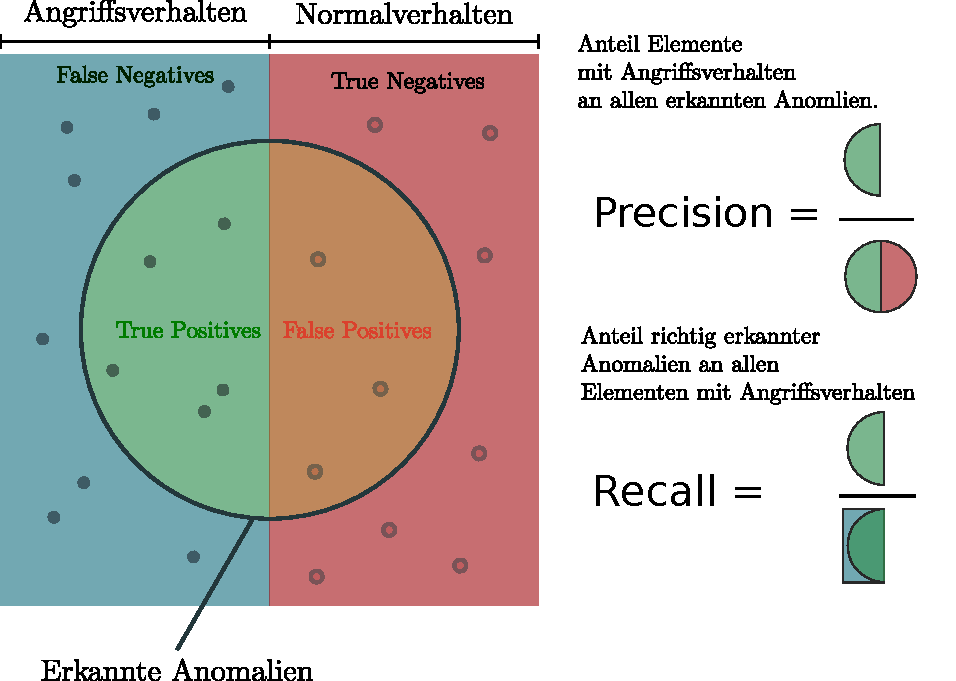
\includegraphics[width=0.75\textwidth]{images/Illustrationen/Precision.pdf}
        \caption[Darstellung Precision und Recall]{Visualisierung der Berechnung der häufig verwendeten Metriken der Precision und des Recalls, bezogen auf die Domäner der \textit{Intrusion Detection}.}\label{fig:metriken}
    \end{figure}
    Diese werden wie in \autoref{fig:metriken} dargestellt berechnet.
    Da der Datensatz aus System Calls besteht bedeutet Recall in diesem Fall, der Anteil an korrekt erkannten bösartigen System Calls, an allen bösartigen System Calls.
    Wie in \autoref{sec:prob_LIDDS} beschrieben liefert der Datensatz allerdings nur den Angriffszeitpunkt und keine Label für jeden einzelnen System Call.
    Also muss jeder System Call nach dem Angriffszeitpunkt als bösartig eingestuft werden, obwohl neben dem Angriffsverhalten noch Normalverhalten stattfindet.
    Wird von einem optimalen Fall ausgegangen, dass alle dem Angriff zugehörigen System Calls einen Alarm auslösen, wird der Recall immer noch sehr niedrig sein und damit keinen realistischen Wert liefern.
    Somit ist auch der F1-Score wenig nützlich, da sich dieser aus Recall und Precision zusammensetzt.
    Es scheint deshalb sinnvoller andere Metriken zur Hand zu nehmen um einheitliche und vom Datensatz unabhängige Messwerte bereitstellen zu können. 
    Da der \ac{LID-DS} aus vielen verschiedenen Aufnahmen besteht kann die Berechnung der Precision und des Recalls auch auf Dateiebene stattfinden.
    Falls mehrere Angriffe in einer Datei vorkommen wird die Berechnung jedoch umständlicher, dies ist im \ac{LID-DS} nicht der Fall.  
    Grundgedanke der Findung einer neuen Metrik muss dabei auch sein einen klaren Praxisbezug zu finden. 
    Dort ist vor allem interessant wieviele Angriffe erkannt werden und nicht wieviele System Calls der Angriffe als bösartig eingestuft werden.
    Zum anderen entscheidet die Anzahl, beziehungsweise die Häufigkeit von Fehlalarmen über die Nutzbarkeit der \acp{IDS}.
    Die \ac{DR} steht für den zuvor beschriebenen Recall auf Dateiebene, also der Anteil der erkannten Angriffe an allen vorkommenden Angriffen.
    Werden alle Aufnahmen mit Angriffsverhalten korrekt erkannt gilt: $\ac{DR}=1$.
    Dabei wird außer Acht gelassen, dass ein Alarm nach dem Angriffszeitpunkt wie in \autoref{sec:prob_LIDDS} beschrieben theoretisch auch ein Fehlalarm sein kann.
    Nur ein Alarm vor dem Angriffszeitpunkt oder in einer Aufnahme ohne Angriffsverhalten wird als Fehlalarm beziehungsweise als \ac{FP} gewertet.
    Zusätzlich gelten alle System Calls solange zu einem Alarm, bis der $ascore$ wieder unter dem Schwellwert $\theta$ liegt.
    Ziel ist es also eine hohe \ac{DR} und eine möglichst geringe \ac{FP}-Rate zu erreichen.
    Um einschätzen zu können welche Konfiguration am besten abgeschnitten hat, ergibt sich eine neue Schwierigkeit.
    Es ist schwierig zu beurteilen welche Konfiguration am besten funktioniert, denn wenn alle System Calls aus dem Datensatz als Angriff erkannt werden, ist $\ac{DR}=1$.
    Eine hohe \ac{DR} alleine ist also wenig aussagekräftig.
    In der Auswertung muss deswegen eine Abwägung zwischen \ac{FP}-Rate und \ac{DR} stattfinden.
    %Eine Angriff gilt dann als erkannt, sofern ein Alarm nach dem Angriffszeitpunkt ausgelöst wird. 
    %Wie in \autoref{sec:LIDDS} beschrieben werden dabei potentiell Fehlalarme als korrekt eingestuft.
    % Das sind im Folgenden die \ac{DR} und die \ac{FP}-Rate

% %*****************************************
\chapter{Implementierung}\label{ch:implementierung}
%*****************************************
Verschiedene Komponenete um Modelle in Python umzusetzen 
zunächst soll auf vorverarbeitung eingegangen werden

\section{Erstellen der Trainingsdaten}
\subsection{w2v}
verschiedene varianten mit ignore thread info
\subsection{Parameterinfo}



\chapter{Ergebnisse}
\label{ch:erg}
\section{Optimale Parameter}

        \paragraph{Architektur}
            versch architekturen:
            Single Small 50 neuronen eine schicht
            Single Big 250 neuronen eine schicht
            multi small 20 neuronen 3 schichten
            multi big 50 neuronrn 3 schichten
            deep erste 50 sonst 20 6 schichten

            singlesmall 43\% von Deep
            insgesamt am schnellsten single small
            wie zu erwarten,  deep am langsamsten

        \paragraph{Hyperparameter}<++>
            aktivierungs funktion
            -> dense layer with softmax or tanh
            batch size
            learning rate
            optimizer

        \paragraph{Ngram Größe}
            ngram größer -> langsamer

        \paragraph{Embedding}

            overhead berechnung embedding, muss allerdings nur einmal berechnet werden
            zu erkennen w2v mit embedding size = 2  und window = 4 wesentlich schneller
            embedding größer -> langsamer

            vergleich ngram
            im schnitt mit ngram gr 2 84\% von ngr 3 und 

            w2v bringt entscheidenden Vorteil gegenüber ohe:
            Jeweils vergleich der selben parameter außer w2v vs ohe:
            Single small w2v nur 30\% der zeit gegenüber single small ohe
            bei mulit w2v sogar nur 13\%
            im mittel über alle architekturen 21.5\% der Zeit von ohe bei verwendung w2v

        \paragraph{Architektur}
            teste eine schicht viele neuronen 
            eine schicht wenige neuronen
            mehrere schichten mehrere neuronen / mit dropout dazwischen
            viele schichten wenige neuronen /mit dropout dazwischen

            auf Grund des zeitlichen Faktors fallen Deep und multibig weg
            Also zu testen:
            Single Small
            Single 
            Multi Small
            Multi 

        \paragraph{Threadinfo}
            Hypothese:
            Threadinfos bringen was

            Einbinden von thread information auf verschiedenen wegen:
            Thread aware ngrams (tan)
            Thread aware ngrams for w2v (tanw2v)
            Thread change flag (tcf)

            varianten:
            tan
            tanw2v
            tcf
            tan tcf
            tan tanw2v
            tcf tanw2v
            tan tanw2v tcf

            ---> welcher dieser varianten am besten?

        \paragraph{Parameter}
            args
            time

            LSTM ohne Threadinfos mit OHE
            LSTM mit W2V ohne Threadinfos (ngram)
            LSTM mit W2V mit Threadinfos (ngram)
            LSTM mit W2V threadaware mit Threadinfos (ngram)
            LSTM mit W2V threadaware mit Threadinfos (ngram) und threadchangeflag
            LSTM mit W2Vthreadaware mit Threadinfos (ngram) und threadchangeflag, spezialtraining
            --> LSTM final

            Manche angriffe verändern Sequenz von syscalls nicht
            Hypothese:
            verwende Parameter um erg zu verb

            LSTM final + strlen
            LSTM final + time delta
            LSTM final + strlen + time delta
\section{LSTM Ansatz}


\section{Extra Parameter}
    \subsection{Timing}\label{sec:Ergebnis_timing}


%*****************************************
\chapter{Folgerungen}\label{ch:folgerungen}
%*****************************************
Nachdem die Ergebnisse der Versuchsreihen vorgestellt wurden, folgt nun eine Bewertung der Ergebnisse.
Dafür werden in \autoref{sec:folgerungen_LSTM} zunächst nur die Ergebnisse des \ac{LSTM} Ansatz besprochen.
Im Anschluß werden in \autoref{sec:folgerungen_extra} die Folgerungen aus den Experimenten mit Extraparametern erörtert. 
Schließlich werden in \autoref{sec:folgerungen_vgl} die Ergebnisse des Vergleichs anderer Arbeiten mit demselben Datensatz besprochen

\section{\NoCaseChange{\ac{LSTM}} Ansatz}\label{sec:folgerungen_LSTM}
\sectionmark{LSTM Ansatz}

Die Ergebnisse beim Einsatz von \acp{LSTM} in anomaliebasierten \acp{HIDS} zeigen zwei Dinge sehr deutlich.
%Der aus der \ac{NLP} bekannte Ansatz kann erfolgreich in der \ac{HIDS} eingesetzt werden.
Erstens, das \ac{LSTM} kann ein Sprachmodell der System Calls erstellen und damit erfolgreich System Calls vorhersagen.
Dies haben auch andere Arbeiten versucht zu zeigen, doch wie zuvor in \autoref{sec:related_nlp} beschrieben, erfolgten die Auswertungen bisher auf veralteten Datensätzen mit praxisfernen Metriken und oft ohne detaillierte Beschreibung des Aufbaus.
Aufgrund dessen kann leider kein direkter Vergleich der Architekturen der \acp{LSTM} gezogen werden.
Die Ergebnisse der Experimente konnten für die N-Gram und Embidding Größe keinen klaren Trend abbilden.
Bei einer N-Gram Größe von $n=10$ und einer Embedding Größe von $e=4$ konnten ähnlich gute Ergebnisse erzielt werden wie bei $n=2$ und $e=4$.\par\medskip

Zweitens zeigt sich allerdings, dass der Berechnungsaufwand gerade bei großem $n$ sehr hoch ist.
Speziell bei sehr großen Szenarien hat dies in dieser Arbeit zu Ressourcenengpässen geführt.
Es konnten, wie zuvor beschrieben, einige Konfigurationen nicht auf dem größten Szenario des \acp{LID-DS} berechnet werden.\par\medskip
Ein weiterer Nachteil der Anomalieerkennung durch ein \ac{LSTM} besteht darin, dass ein GPU für eine effiziente Berechnung nötig ist.
Hinzu kommt, dass mit einem \ac{LSTM} eine Parallelisierung nur geringfügigen Einfluss auf die Berechnungszeit hat.
Grundproblem dabei ist die Rekurrenz des Netzes. 
Die Ausgabe des letzten Zeitschrittes muss bekannt sein, um die Ausgabe des aktuellen Zeitschrittes berechnen zu können.
Aus den vorliegenden Ergebnissen kann, im Vergleich zur \ac{STIDE} Implementierung von Grimmer et al.~\cite{IDSTHREADGRIMMER2021}, der Einsatz von \acp{LSTM} in der beschriebenen Architektur, ohne die Verwendung von zusätzlichen Parametern, keine Verbesserung erzielen.\par\medskip

Daraus lässt sich schließen, dass \acp{LSTM} ohne die Verwendung zusätzlicher Parameter aufgrund des mit der Berechnung verbundenen Mehraufwands keine nennenswerten Vorteile bringen konnte.
% Das liegt wahrscheinlich daran, dass die Muster in den Sequenzen nicht komplex genug sind, dass die Aufwendige Implementierung der \acp{LSTM} zu trage kommen.

Wie dies unter der Verwendung von Extraparametern aussieht wird im Folgenden betrachtet.

\section{Einsatz von Extraparametern}\label{sec:folgerungen_extra}

Wie in \autoref{sec:erg_LSTM_extra} beschrieben, kann eine deutliche Verbesserung der \ac{DR} sowie  der \ac{FP}-Rate mit dem Einsatz verschiedener Extraparameter erzielt werden.
So sind $9$ unter den besten $10$ Ergebnissen bezüglich \ac{DR} und $7$ bezüglich \ac{FP}-Rate Konfigurationen mit mindestens einem Extraparameter.\par\medskip

Im Vergleich zu den Ergebnissen ohne Extraparametern ist hier ein Trend zu größeren N-Grammen erkennbar.
Es ist nur noch insgesamt eine Konfiguration unter den besten zehn Ergebnissen bezüglich \ac{DR} und \ac{FP} mit einer N-Gram Größe von $2$.
Im Vergleich zu insgesamt sieben \marginpar{drei bezüglich \ac{DR}, vier bezüglich \ac{FP}} der besten zehn bei Konfigurationen ohne Verwendung von Extraparametern.
Woraus sich schließen lässt, dass bei komplexeren Eingaben größere N-Gramme bessere Ergebnisse liefern.\par\medskip

Auffällig sind auch die Verteilungen der N-Gram Größen.
Unter Einsatz der Extraparameter kommt bezüglich \ac{DR} und \acp{FP} einmal eine Konfiguration mit $n<6$ vor, während dies bei Konfigurationen ohne Extraparametern sieben mal der Fall ist.\par\medskip

Abschließend lässt sich sagen, dass $n=10$ und $e=4$ sowie $n=6$ und $e=8$ die besten Konfigurationen bezüglich \ac{DR} und \ac{FP} darstellen.
Zusätzlich konnte zwar keine eindeutig beste Konfiguration für die Kombination der zusätzlichen Parametern gefunden werden, aber fast alle Kombinationen konnten eine Verbesserung der Ergebnisse erzielen.

\section{Vergleich anderer Arbeiten}\label{sec:folgerungen_vgl}

Der Vergleich mit anderen \ac{LSTM}-basierenden Arbeiten ist, wie bereits erwähnt, aufgrund der uneinheitlichen Datensätze schwierig.
Dennoch kann ein Vergleich zu der Arbeit von Grimmer et al.~\cite{IDSTHREADGRIMMER2021} gezogen werden.
Hierfür wurden die besten Konfiguration sowie das von Grimmer et al.~\cite{IDSTHREADGRIMMER2021} eingeführte 5-Level-Modell herangezogen.
Im Direktvergleich der besten Konfiguration in \autoref{tab:LSTM_stide_erg} ist signifikanter Rückgang der \acp{FP} zu erkennen, in \autoref{tab:LSTM_lvl} ist dies nicht mehr erkennbar.
Das \ac{LSTM} kann mit einer Auswahl an Algorithmen auf allen Leveln bis auf Level $5$ konkurrieren.
Dabei verwenden diese Algorithmen keine Extraparameter.
Der entworfene anomaliebasierte \ac{HIDS} Ansatz unter Verwendung eines \acp{LSTM} kann somit mit den in der Forschung verwendeten Algorithmen konkurrieren.
Wie die erlangten Erkenntnisse in Zukunft weiter ihren Einsatz finden können, soll im folgenden Kapitel untersucht werden.

\chapter{Zusammenfassung und Ausblick}\label{ch:schluss}

IT-Sicherheit ist in der Praxis oft einen Schritt hinter den Angriffen zurück.
Dies liegt daran, dass Verteidigungssysteme üblicherweise versuchen Angriffe anhand ihrer Signaturen zu erkennen.
Sind die Angriffe noch nicht bekannt, so können auch noch keine Signaturen dafür existieren.
Das sorgt dafür, dass sie auch nicht erkannt werden können.
Gleiches gilt für die meisten Abwandlungen von bereits bekannten Angriffen.
Um den Angriffen nicht immer hinterher zu sein, wird versucht mit anomaliebasierten Verteidigungssystemen auch unbekannte Angriffe zu erkennen.
Statt eine Liste von Angriffen ständig up-to-date halten zu müssen, wird versucht Muster des Normalverhaltens zu erlernen.
Eine Abweichung des Normalverhaltens wird dann als Angriff gewertet und ermöglicht es, zeitnahe weitere Schritte einzuleiten.

\section{Zusammenfassung}

Um die Sicherheit von Computersystemen zu gewährleisten, werden häufig \acp{IDS} in die IT-Infrastruktur eingepflegt.
Häufig werden \ac{NIDS} verwendet, welche Netzwerkdaten untersuchen und damit mehrere Hosts gleichzeitig überwachen.
Um Angriffe auf einzelnen Hosts zu erkennen, reichen diese meist nicht aus.
\acp{HIDS} können IT-Sicherheitssysteme um diese Fähigkeit erweitern.
Seit mehr als 20 Jahren werden \acp{HIDS} in der Forschung behandelt, wobei sich das Untersuchen von System Call Daten als vielversprechend herausgestellt hat.
Seit dem Beginn der Forschung wurden verschiedene Algorithmen sowie Datensätze, auf welchen diese ausgewertet werden können, präsentiert.
Da aber viele Datensätze Unzulänglichkeiten aufweisen, leidet die Vergleichbarkeit der Ergebnisse stark.
Der auf modernen Systemen aufgezeichnete \ac{LID-DS} beseitigt einige dieser Unzulänglichkeiten.
Diese Arbeit beschäftigt sich speziell mit \acp{HIDS}, welche Anomalien in Sytem Call Streams des \ac{LID-DS} erkennen. 
In der  ersten Iteration wird die Sequenz der System Calls betrachtet, wobei dafür die Sequenz der System Call Namen verwendet wird.
Dabei bietet es sich an, von etablierten Verfahren der Mustererkennung zu profitieren.
Ein Bereich der Mustererkennung, welcher großen Fortschritt erfahren hat, ist die \ac{NLP}.
Es stellt sich also die Frage, ob bestimmte Verfahren, die in der \ac{NLP} eingesetzt werden, auch im Bereich der \ac{HIDS} erfolgreich sind.
Speziell die \acp{LSTM} zeigten sich in der Sprachverarbeitung sowie in der Analyse von Zeitreihendaten als effektiv.
\acp{LSTM} haben gegenüber vielen anderen Algorithmen die in der Forschung bisher eingesetzt wurden einen Vorteil.
Sie beziehen zuvor gesehene Eingaben in die Klassifizierung der aktuellen Eingabe mit ein, kennen also den Kontext der aktuellen Eingabe.
Es wurde in dieser Arbeit gezeigt, dass sich die Fortschritte der \ac{NLP} in Form von \acp{LSTM} auf die anomaliebasierte \ac{HIDS} übertragen lassen.
Um die System Call Namen sinnvoll für das \ac{LSTM} darzustellen, wird auf ein ebenfalls aus der \ac{NLP} stammendes Verfahren zurückgegriffen.
Das \ac{W2V}-Verfahren stellt nicht nur ein Lookup-Table für System Calls dar, sondern kodiert auch Kontextinformationen der System Calls.
Um die Ergebnisse des entworfenen Algorithmus weiter zu verbessern, werden neue Verfahren zur Kodierung zusätzlicher Informationen der System Calls vorgestellt.
Zum einen werden dafür die Rückgabewerte bestimmter lesender und schreibender System Calls verwendet. 
Dies wird erreicht, indem für jede Kategorie, zum Beispiel lesende System Calls, das Maximum der gelesenen Bytes aus den Trainingsdaten ermittelt wird.
Mit dem ermittelten Maximum werden dann die Werte aus den Testdaten normalisiert.
Und zum anderen werden auf gleiche Weise die zeitlichen Abstände zwischen zwei System Calls innerhalb eines Threads normalisiert und dienen so als Eingabe für das \ac{LSTM}.
In einem weiteren Feature werden die von Grimmer et al.~\cite{IDSTHREADGRIMMER2021} präsentierten \textit{Thread aware} N-Gramme für Algorithmen mit Kontextwissen erweitert.
Da es für \acp{RNN} von Bedeutung ist, was für eine Eingabe im letzten Zeitschritt gesehen wurde, soll dem \ac{LSTM} ein Wechsel des Threads und damit ein Wechsel des Kontextes mitgeteilt werden.
Dieses Feature wird also nur Algorithmen einen Vorteil bringen, welche den Kontext der Eingaben miteinbeziehen.
Um zu überprüfen, ob und mit welcher Konfiguration sich die beschriebenen Verfahren als erfolgreich erweisen, werden ausführliche Experimente auf dem \ac{LID-DS} durchgeführt.
Die Auswertung der Ergebnisse bringt zwei Probleme mit sich.
Erstens sind einige bekannte und verbreitete Metriken zur Auswertung von neuronalen Netzen mit dem vorhandenen Datensatz nicht umzusetzen.
Deswegen werden in der Arbeit \ac{FP}-Rate und \ac{DR} verwendet. 
Diese werden auch in anderen Arbeiten auf diesem Datensatz angewandt und bieten zusätzlich einen größere Praxisnähe.
Zweitens ist die Auswahl der besten Konfigurationen auf der Grundlage von zwei Kriterien ohne Gewichtung der Kriterien nicht möglich.
Es werden verschiedene Eingabegrößen und Konfigurationen der Extraparameter untersucht.
Eine klare Tendenz für optimale Eingabegrößen oder Konfiguration sind dabei nicht zu erkennen.
Dennoch kann gezeigt werden, dass die \acp{LSTM} konkurrenzfähige, aber nicht signifikant bessere Ergebnisse liefern, insbesondere wenn die zusätzlichen Parameter hinzugefügt werden.
Der größte Nachteil des präsentierten \ac{HIDS} Verfahren besteht in der aufwendigen Berechnung der \acp{LSTM}.
Es zeigt sich also, dass sich der Erfolg der \acp{LSTM} in der \ac{NLP} auf die Erkennung von Anomalien in der Cyber-Sicherheit übertragen lässt, dabei aber auch neue Schwierigkeiten mit sich bringt.
Auch die Zunahme von Extraparametern der System Calls erzielt eine klare Verbesserung.
%Die Arbeit liefert damit vielversprechende Ansätze für weitere Forschung in diesem Bereich.

\section{Ausblick}
Wie beschrieben kann der \ac{LSTM} Ansatz zwar keine offensichtliche Verbesserung der Ergebnisse erreichen, doch zeigt er, dass eventuell auch weitere Lösungsansätze aus der \ac{NLP} auf die Anomalieerkennung übertragen werden können.
Eine Möglichkeit diese Ergebnisse zu verbessern, könnten in Konfigurationen bestehen, die noch nicht getesteten wurden.
So könnten die Auswirkungen von größeren \ac{LSTM}-Architekturen auf die Ergebnisse untersucht werden.
Dies wird aber die Berechnungszeiten noch weiter erhöhen.
Ein Punkt gegen die weitere Untersuchung von \acp{LSTM} in dieser Domäne besteht darin, dass Transformer sich bereits bei den meisten Übersetzungs-  und Sprachgenerierungsprogrammen  gegenüber den \acp{LSTM} durchgesetzt haben. 
Denn sie ermöglichen wie die \acp{LSTM} eine Verarbeitung der System Calls mit Einbindung des Kontexts.
Gleichzeitig kann die Berechnung der Eingaben in Transformern besser parallelisiert werden.
Dieser Ansatz könnte die Vorteile der \acp{LSTM} ausspielen und einen erheblichen Geschwindigkeitsvorteil bringen.

Die Erkenntnisse der Arbeit bezüglich des Entwurfs neuer Kodierungen für Extraparameter der System Calls könnte sich hingegen direkt auf weitere Arbeiten auswirken.
So kann vielleicht der Einsatz der Extraparameter in Zukunft eine Verbesserung der Ergebnisse des \ac{STIDE} oder anderen Algorithmen erzielen.
Insbesondere können weitere kontextsensitive Algorithmen durch die Erweiterung der \textit{Thread Aware} N-Gramme profitieren. 
Aber die präsentierten zusätzlichen Parameter sind ebenfalls noch erweiterbar.
So können noch weitere Normalisierungen von System Call Rückgabewerten erfolgen.
Zum Beispiel wurde der System Call \textit{send} bisher noch nicht mit einbezogen.
Auch weitere Gruppierungen von System Calls oder eventuell das Auflösen von Gruppierungen sollte in weiteren Arbeiten untersucht werden.
Es kann zwar davon ausgegangen werden, dass sich die Erfolge der Extraparameter im Zusammenhang mit den \ac{LSTM} Ansatz nicht eins zu eins auf Ansätze wie den \ac{STIDE} Algorithmus übertragen lassen, dennoch wurden in dieser Arbeit neue Kodierungsansätze präsentiert, die zur breiteren Nutzung von zusätzlichen Parametern beitragen.


%\include{multiToC} % <--- just debug stuff, ignore for your documents
% ********************************************************************
% Backmatter
%*******************************************************
\appendix
%\renewcommand{\thechapter}{\alph{chapter}}
%\cleardoublepage
%\part{Appendix}
%%********************************************************************
% Appendix
%*******************************************************
% If problems with the headers: get headings in appendix etc. right
%\markboth{\spacedlowsmallcaps{Appendix}}{\spacedlowsmallcaps{Appendix}}
\chapter{Appendix Test}
Lorem ipsum at nusquam appellantur his, ut eos erant homero
concludaturque. Albucius appellantur deterruisset id eam, vivendum
partiendo dissentiet ei ius. Vis melius facilisis ea, sea id convenire
referrentur, takimata adolescens ex duo. Ei harum argumentum per. Eam
vidit exerci appetere ad, ut vel zzril intellegam interpretaris.
\graffito{More dummy text.}

%Errem omnium ea per, pro congue populo ornatus cu, ex qui dicant
%nemore melius. No pri diam iriure euismod. Graecis eleifend
%appellantur quo id. Id corpora inimicus nam, facer nonummy ne pro,
%kasd repudiandae ei mei. Mea menandri mediocrem dissentiet cu, ex
%nominati imperdiet nec, sea odio duis vocent ei. Tempor everti
%appareat cu ius, ridens audiam an qui, aliquid admodum conceptam ne
%qui. Vis ea melius nostrum, mel alienum euripidis eu.

\section{Appendix Section Test}
Test: \autoref{tab:moreexample} (This reference should have a
lowercase, small caps \spacedlowsmallcaps{A} if the option
\texttt{floatperchapter} is activated, just as in the table itself
 $\rightarrow$ however, this does not work at the moment.)

\begin{table}[h]
    \myfloatalign
    \begin{tabularx}{\textwidth}{Xll} \toprule
        \tableheadline{labitur bonorum pri no} & \tableheadline{que vista}
        & \tableheadline{human} \\ \midrule
        fastidii ea ius & germano &  demonstratea \\
        suscipit instructior & titulo & personas \\
        %postulant quo & westeuropee & sanctificatec \\
        \midrule
        quaestio philosophia & facto & demonstrated \\
        %autem vulputate ex & parola & romanic \\
        %usu mucius iisque & studio & sanctificatef \\
        \bottomrule
    \end{tabularx}
    \caption[Autem usu id]{Autem usu id.}
    \label{tab:moreexample}
\end{table}

%Nulla fastidii ea ius, exerci suscipit instructior te nam, in ullum
%postulant quo. Congue quaestio philosophia his at, sea odio autem
%vulputate ex. Cu usu mucius iisque voluptua. Sit maiorum propriae at,
%ea cum primis intellegat. Hinc cotidieque reprehendunt eu nec. Autem
%timeam deleniti usu id, in nec nibh altera.




\section{Another Appendix Section Test}
Equidem detraxit cu nam, vix eu delenit periculis. Eos ut vero
constituto, no vidit propriae complectitur sea. Diceret nonummy in
has, no qui eligendi recteque consetetur. Mel eu dictas suscipiantur,
et sed placerat oporteat. At ipsum electram mei, ad aeque atomorum
mea. There is also a useless Pascal listing below: \autoref{lst:useless}.

\begin{lstlisting}[float=b,language=Pascal,frame=tb,caption={A floating example (\texttt{listings} manual)},label=lst:useless]
for i:=maxint downto 0 do
begin
{ do nothing }
end;
\end{lstlisting}

%Ei solet nemore consectetuer nam. Ad eam porro impetus, te choro omnes
%evertitur mel. Molestie conclusionemque vel at, no qui omittam
%expetenda efficiendi. Eu quo nobis offendit, verterem scriptorem ne
%vix.


%********************************************************************
% Other Stuff in the Back
%*******************************************************
%********************************************************************
% Bibliography
%*******************************************************
% work-around to have small caps also here in the headline
% https://tex.stackexchange.com/questions/188126/wrong-header-in-bibliography-classicthesis
% Thanks to Enrico Gregorio
\defbibheading{bibintoc}[\bibname]{%
  \phantomsection
  \manualmark
  \markboth{\spacedlowsmallcaps{#1}}{\spacedlowsmallcaps{#1}}%
  \addtocontents{toc}{\protect\vspace{\beforebibskip}}%
  \addcontentsline{toc}{chapter}{\tocEntry{#1}}%
  \chapter*{#1}%
}
\printbibliography[heading=bibintoc]

% Old version, will be removed later
% work-around to have small caps also here in the headline
%\manualmark
%\markboth{\spacedlowsmallcaps{\bibname}}{\spacedlowsmallcaps{\bibname}} % work-around to have small caps also
%\phantomsection
%\refstepcounter{dummy}
%\addtocontents{toc}{\protect\vspace{\beforebibskip}} % to have the bib a bit from the rest in the toc
%\addcontentsline{toc}{chapter}{\tocEntry{\bibname}}
%\label{app:bibliography}
%\printbibliography

%\cleardoublepage%*******************************************************
% Declaration
%*******************************************************
\pdfbookmark[0]{Declaration}{declaration}
\chapter*{Declaration}
\thispagestyle{empty}
Put your declaration here.
\bigskip

\noindent\textit{\myLocation, \myTime}

\smallskip

\begin{flushright}
    \begin{tabular}{m{5cm}}
        \\ \hline
        \centering\myName \\
    \end{tabular}
\end{flushright}

%\cleardoublepage\pagestyle{empty}

\hfill

\vfill


\pdfbookmark[0]{Colophon}{colophon}
\section*{Colophon}
This document was typeset using the typographical look-and-feel \texttt{classicthesis} developed by Andr\'e Miede and Ivo Pletikosić.
The style was inspired by Robert Bringhurst's seminal book on typography ``\emph{The Elements of Typographic Style}''.
\texttt{classicthesis} is available for both \LaTeX\ and \mLyX:
\begin{center}
\url{https://bitbucket.org/amiede/classicthesis/}
\end{center}
Happy users of \texttt{classicthesis} usually send a real postcard to the author, a collection of postcards received so far is featured here:
\begin{center}
\url{http://postcards.miede.de/}
\end{center}
Thank you very much for your feedback and contribution.

\bigskip

\noindent\finalVersionString

%Hermann Zapf's \emph{Palatino} and \emph{Euler} type faces (Type~1 PostScript fonts \emph{URW
%Palladio L} and \emph{FPL}) are used. The ``typewriter'' text is typeset in \emph{Bera Mono},
%originally developed by Bitstream, Inc. as ``Bitstream Vera''. (Type~1 PostScript fonts were made
%available by Malte Rosenau and
%Ulrich Dirr.)

%\paragraph{note:} The custom size of the textblock was calculated
%using the directions given by Mr. Bringhurst (pages 26--29 and
%175/176). 10~pt Palatino needs  133.21~pt for the string
%``abcdefghijklmnopqrstuvwxyz''. This yields a good line length between
%24--26~pc (288--312~pt). Using a ``\emph{double square textblock}''
%with a 1:2 ratio this results in a textblock of 312:624~pt (which
%includes the headline in this design). A good alternative would be the
%``\emph{golden section textblock}'' with a ratio of 1:1.62, here
%312:505.44~pt. For comparison, \texttt{DIV9} of the \texttt{typearea}
%package results in a line length of 389~pt (32.4~pc), which is by far
%too long. However, this information will only be of interest for
%hardcore pseudo-typographers like me.%
%
%To make your own calculations, use the following commands and look up
%the corresponding lengths in the book:
%\begin{verbatim}
%    \settowidth{\abcd}{abcdefghijklmnopqrstuvwxyz}
%    \the\abcd\ % prints the value of the length
%\end{verbatim}
%Please see the file \texttt{classicthesis.sty} for some precalculated
%values for Palatino and Minion.
%
%    \settowidth{\abcd}{abcdefghijklmnopqrstuvwxyz}
%    \the\abcd\ % prints the value of the length

% ********************************************************************
% Game Over: Restore, Restart, or Quit?
%*******************************************************
\end{document}
% ********************************************************************
